\documentclass[12pt,a4paper]{report}

\usepackage{latexsym,amssymb,amsmath}
\usepackage{mathdefs}
\usepackage{multirow}
\usepackage{booktabs}
\usepackage{enumerate}
\usepackage[T1]{fontenc}
%\usepackage{graphicx}
\usepackage{booktabs}
\usepackage{rotating}
\usepackage{multirow}
%\usepackage{caption}

\usepackage{cleveref}
\usepackage{enumerate}
\usepackage{framed}
\usepackage{amsthm}
\usepackage{makeidx}
\usepackage{xfrac}
\usepackage{graphicx}
\usepackage{caption}
\usepackage{subcaption}
\usepackage{epstopdf}
\usepackage{booktabs}
\usepackage{ltxtable} 


%%%%%% Size %%%%%%%%%%%%%%%%%%%%%%%%%%%%%%%%%%%%%%%%%%%%%%%%

% START OF DEFINITIONS
%%%%%% Size %%%%%%%%%%%%%%%%%%%%%%%%%%%%%%%%%%%%%%%%%%%%%%%

\setlength{\marginparwidth}{0in} \setlength{\marginparsep}{0in}
\setlength{\oddsidemargin}{0in} \setlength{\evensidemargin}{0in}
\setlength{\textwidth}{6.in} \setlength{\topmargin}{0in}
\setlength{\textheight}{9.in}

%********************** General Definitions ******************************

\newtheorem{theorem}{Theorem}[section]
\newtheorem{definition}{Definition}[section]
\newtheorem{example}{Example}[section]
\newtheorem{proposition}{Proposition}[section]
\newtheorem{remark}{Remark}[section]%
\newtheorem{lemma}{Lemma}[section]
\newtheorem{assumption}{Assumption}[section]
\newtheorem{corollary}{Corollary}[section]
\def\nr{\par \noindent}
% END OF DEFINITIONS
%******************* Counters etc ************************************* %
\renewcommand{\baselinestretch}{1.2}

%\renewcommand{\theequation}{\thesection.\arabic{equation}} % Equation numbering with subsections
\newcommand{\sect}[1]{\setcounter{equation}{0}\section{#1}} %
\def\theequation{\thesection.\arabic{equation}}


%\newcommand{\qed}{\hfill $\Box$ \nr \medskip} %End of proof
%\newcommand{\qed}{\hfill\BlackBox\\[2mm]} % End of proof.

% Different font in captions
\newcommand{\captionfonts}{\small}


\makeatletter  % Allow the use of @ in command names
\long\def\@makecaption#1#2{%
  \vskip\abovecaptionskip
  \sbox\@tempboxa{{\captionfonts #1: #2}}%
  \ifdim \wd\@tempboxa >\hsize
    {\captionfonts #1: #2\par}
  \else
    \hbox to\hsize{\hfil\box\@tempboxa\hfil}%
  \fi
  \vskip\belowcaptionskip}
\makeatother   % Cancel the effect of \makeatletter


\newcommand{\nn}{\mathbb{N}} %Nonnegative integers
\newcommand{\rr}{\mathbb{R}} %Real numbers
\newcommand{\norm}[1]{\left\Vert {#1} \right\Vert} %Norm
\def\abs#1{\left\lvert#1\right\rvert}

%*******************************************************

% etc
%

\begin{document}

%
%--------- Title
%

 \thispagestyle{empty}

\vspace{3cm}
\begin{center}
Tel-Aviv University\\
Raymond and Beverly Sackler Faculty of Exact Sciences\\
\vspace{2.5cm} {\bf A Novel Class of Globally Convergent Algorithms\\ For Clustering Problems}\\
 \vspace{2.5cm}

Thesis submitted in partial fulfillment of graduation requirements\\
for a degree of M.Sc. at Tel-Aviv University\\
\vspace{2cm}
Tel-Aviv University\\
School of Mathematical Sciences\\
Department of Statistics and Operations Research\\
\vspace{2cm}
By\\
Sergey Voldman\\
\vspace{2cm}
The research work in this thesis has been conducted\\
under the supervision of Prof. Marc Teboulle\\
and Prof. Shoham Sabach\\
\vspace{2cm}
January 2016\\
\end{center}

\nobreak

%
%--------- Start numbering preface in roman
%
\pagenumbering{roman}
%
%--------- Preface
%
\setcounter{page}{3}
\chapter*{Abstract}

This thesis presents some of the very best...



\addcontentsline{toc}{chapter}{Abstract}

\chapter*{Acknowledgements}

I would like to thank Prof. Marc Teboulle for introducing me to the interesting world of continuous optimization during my graduate studies.    I would also like to thank Prof. Teboulle for the suggestion to research the clustering problem and his helpful initial ideas how to tackle this complex and important problem.

In addition I would like to thank Prof. Shoham Sabach for his dedication and patience in helping me to complete this thesis, especially in his helpful comments during the many revisions of this thesis.

I thank Tel-Aviv university for the financial aid during the work on this thesis.

Finally I would like to express my family for their support and encouragement during the work on this thesis.

Sergey Voldman

\addcontentsline{toc}{chapter}{Acknowledgements}

\nobreak

%
\tableofcontents
\newpage

\listoftables
\newpage

\listoffigures
\newpage

%
%--------- Start from Page 1
%
\pagenumbering{arabic}



 \chapter{Introduction} \label{intro}

\noindent \noindent \hrulefill

\section{Background and Motivation}

The clustering problem is the task of grouping objects which are similar. It consists of partitioning a dataset into subsets, called clusters, such that the data points in each cluster are similar with respect to a specific criteria. 

The clustering problem is a fundamental problem in the machine learning field, and it arises in wide scope of applications, such as data mining, pattern recognition, information retrieval and many others. For example, in image segmentation, one is interested in partitioning the pixels of an image into objects, where each pixel can be described via its location in the image and its color given in RGB format. Another example is learning the probability density of some data, where the data is assumed to be drawn from a mixtures of distributions. Each partition of the data is represented by a unimodal probability density model, and a summation of all the cluster models gives a multimodal density for the entire dataset. Vector quantization is yet another example, where large sets of points are represented by their centroid point. This method can be used for data compression, data correction and pattern recognition.

There are several categories of clustering methods, each has a direct impact on the final clustering structure.
\begin{enumerate}[(i)]
	\item Hierarchical versus partitioning clustering. In partitioning clustering the dataset is divided into clusters, whereas in hierarchical clustering each cluster may have sub-clusters, thus forming a tree which leaves are the single points of the dataset.
	\item Hard versus soft and fuzzy clustering. In hard clustering each data point is assigned to single cluster, versus a soft clustering where each point may be assigned to more than one cluster, hence clusters may overlap. In fuzzy clustering for each point there is a distribution that describes the probability of a point to be part of a certain cluster.
	\item Complete versus partial clustering. In complete clustering all points in the dataset are assigned to clusters, whereas in partial clustering some points may be intentionally skipped and are not being assigned to a cluster.
\end{enumerate}

Finding the optimal partition of a fixed number of clusters for some given dataset is known to be a NP-hard problem, and hence cannot be solved efficiently. Most algorithms seek to minimize some mathematical criteria, and usually achieve local rather than global minimum solution. In this work we focus on partitioning clustering, where the number of clusters in known in advance. Most partitioning clustering methods iteratively update the cluster centers, and hence they are often referred as center-based clustering methods.

We introduce few notations for the upcoming discussion. Let $\mathcal{A}= \left\lbrace a^1, a^2, \ldots ,a^m \right\rbrace$ be a given set of points in $\mathbb{R}^n$, and let $1 < k < m$ be a fixed given number of clusters. The clustering problem consists of partitioning the dataset $\mathcal{A}$ into $k$ subsets $\left\lbrace C^1, C^2, \ldots ,C^k \right\rbrace$, called clusters. For each $l=1, 2, \ldots ,k$, the cluster $C^l$ is represented by its center $x^l \in \mathbb{R}^n$. We describe several well-known center-based clustering algorithms.
\begin{enumerate}[(i)]
	\item The k-means algorithm. This algorithm is probably the most famous within the clustering scope, and dates back to MacQueen (1967). The k-means algorithm partitions the data into $k$ sets. The solution is then a set of $k$ centers, each of which is located at the centroid of the data for which it is the closest center. The k-means algorithm performs hard clustering, and each point is labeled according to its closest center. This algorithm can be discribed as an optimization algorithm (see precise details below) which minimizes the following objective function
	\begin{equation*}
		f_{KM}(x) = \sum\limits_{i=1}^{m}\min\limits_{1 \le l \le k} \norm{a^i-x^l}^2.
	\end{equation*}
	The simplicity of the algorithm both in the theoretical and implementation aspects made it very popular.
	\item Fuzzy k-means (FKM) algorithm. The FKM algorithm is a soft clustering method. For each data point the result of the FKM algorithm is a distribution of membership over the clusters. The objective function that the FKM algorithm minimizes is
	\begin{equation*}
		f_{FKM}(x) = \sum\limits_{i=1}^{m}\sum\limits_{l=1}^{k}(w^i_l)^\beta \norm{a^i-x^l}^2.
	\end{equation*}
	The parameter $w^i_l$ denotes the probability that data point $a^i$ is assigned to cluster $x^l$, thus it is under the constraints $\sum_{l=1}^{k} w^i_l = 1$ for all $1 \leq i \leq m$ and $w^i_l \geq 0$. The parameter $\beta > 1$ governs the "fuzzy partition". Setting $\beta = 1$ results in the standard k-means algorithm (see \Cref{State_Clustering_Reformulation} for more details).
	\item Expectation-Maximization (EM) algorithm. The EM algorithm is used extensively in statistical estimation problems for learning mixtures of distributions. It is a soft clustering algorithm. The objective function that EM maximizes is 
	\begin{equation*}
		f_{EM} = \sum\limits_{i=1}^{m} \log \left( \sum\limits_{l=1}^{k} p\left(a^i|x^l\right) p\left(x^l\right) \right),
	\end{equation*}
	where  $p\left(a^i|x^l\right)$ is the probability of $a^i$ given that it is generated by the Gaussian distribution with center $x^l$ and $p\left(x^l\right)$ is the prior probability of center $x^l$.
\end{enumerate}
An interesting paper of Teboulle \cite{T2007} shows that these center-based clustering algorithms can be recovered from the proposed continuous optimization framework. The smoothing methodologies for the clustering problem are based on nonlinear means and on approximation of appropriate asymptotic functions.

Most of the existing clustering methods are sensitive to the starting point, namely choosing different starting point result in significant changes in the final clustering. There are plethora of heuristic initialization methods. One such initialization method is to choose $k$ random data points as staring centers, assuming uniform distribution or some other prior distribution on the data. Another popular method is k-means++, where the first center is chosen at random from the dataset, and for each $2 \leq l \leq k$, the center $x^l$ is the furthest data point from the data points chosen so far.

We begin this work with a formulation of the clustering problem which consists of minimizing the sum of finite collection of min-functions. This is a nonsmooth and nonconvex optimization problem, in its most general case. The clustering problem is given by
\begin{equation}
	\min\limits_{x \in \mathbb{R}^{nk}} \left\lbrace F(x) := \sum\limits_{i=1}^{m} \min\limits_{1 \le l \le k} d(x^l,a^i) \right\rbrace , \label{StateEq1}
\end{equation}
where $x=\left( x^1,x^2, \ldots, x^k \right) \in \rr^{nk}$ with $\textit{d}(\cdot ,\cdot)$ being a distance-like function.

We focus on two cases of distance-like functions. The first is the squared Euclidean norm, which is the standard proximity measure used in the k-means algorithm. For this case, we derive an equivalent smooth optimization problem for the clustering problem presented in (\ref{StateEq1}) and prove convergence result for the suggested algorithm via the methodology which was recently developed in \cite{BST2014} and will be discussed in great details below. The second distance-like function that we study is the Euclidean norm. In this case we present an approximation model, in order to overcome the lack of smoothness in the problem. Then we propose an algorithm to solve the approximated model which combines ideas which were used in the squared Euclidean case \textbf{????}. We present numeric experiments, that show the superiority of the Euclidean norm distance function for datasets in which the data points are spread relatively sparsely form their centers.

The lack of smoothness in this formulation can be overcome, yet the nonconvex nature of the clustering problem will accompany the discussions throughout this work. Significant amount of studies have been made on convex models, even though in many cases the original optimization problem is nonconvex. To overcome the lack of convexity, one of the common approaches is usually achieved by considering a convex relaxation of the original problem. In this thesis we take a different route and consider the problem in its original nonconvex form. Very recently this complicated route became more relevant and interesting thanks to few papers which pave the way for dealing with nonconvex problems using sophisticated mathematical tools as will be explained later.


\section{Outline and Contributions of The Thesis}

Our main objectives and contributions in this thesis are as follows:

\begin{itemize}
  \item To reformulate the clustering problem starting from its usual discrete form into a continuous formulation, which enable to treat the problem with powerful continuous optimization tools.
  \item To demonstrate the usefulness of KL theory and the general methodology developed in \cite{BST2014} to tackle the clustering problem.
  \item To develop algorithms that address the clustering problem with two different distance-like functions and examine the superiority of each variation with appropriate datasets.
  \item To prove the convergence of k-means to a critical point.
\end{itemize}

We outline now the contents of this thesis. In chapter 2 we transform the initial formulation  of the clustering problem into a smooth one. In addition, we introduce the KL theory and the general methodology that will be used in our analysis of the proposed algorithms. 

Chapters 3 and 4 present the algorithms that tackle the clustering problem with squared Euclidean norm distance-like function and with the standard Euclidean norm distance function, respectively. For each algorithm, we prove the convergence of the sequences it produces to a critical points of the objective function.

In section 5 we prove the convergence of k-means algorithm to a critical point and under additional assumption extend the convergence to a local minimum. Finally, in Section 6 we compare the performance of these algorithm according to some common criteria.

\section{Notation and Terminology}

The following notations will be used throughout this thesis

\begin{table}[htbp]\caption{Table of Notations}
\begin{center}% used the environment to augment the vertical space
% between the caption and the table
\begin{tabular}{r p{13cm} }
\hline
$\mathcal{A}$ & dataset for clustering of size $m$\\
$k$  & the number of clusters\\
$x^l$ & center of cluster $l$, for each $l=1,2,\ldots,k$\\
$\left\langle\cdot,\cdot\right\rangle$ & the standard dot product in Euclidean space, that is $\left\langle u,v \right\rangle = \sum\limits_{i=1}^{d} u_l v_l$\\
$\norm{\cdot}$ & Euclidean norm $\norm{x}=\sqrt{\sum\limits_{l=1}^{d} {x_l}^2}$\\
$\Delta$  & the simplex i.e., $\Delta = \left\lbrace u \in \mathbb{R}^d : \sum\limits_{l=1}^{d} u_l = 1, \: u \geq 0 \right\rbrace$\\
$\delta_{S}(\cdot)$  & delta function of set $S \subset \rr^d$, which is defined to be $0$ in $S$ and $\infty$ otherwise\\
dom $\sigma$ & domain of function $\sigma$, which is all vectors $v$ such that $\sigma(v) < \infty$\\
$\partial\sigma$ & subdifferential of function $\sigma$ (see \Cref{subdiff_def})\\
crit $\sigma$ & set of all critical points of function $\sigma$, that is all vectors $v$ such that $0 \in \partial\sigma(v)$\\
dist$(u,S)$ & distance function, for any point $u \in \rr^d$ and set $S \in \rr^d$, dist$(u,S):=\inf\left\lbrace \norm{u-v} : v \in S \right\rbrace$\\ 
\hline
\end{tabular}
\end{center}
\label{tab:TableOfNotations}
\end{table}



 \chapter{Problem Reformulation and Mathematical Tools} \label{Chptr2}

\noindent \noindent \hrulefill

Transforming the initial discrete clustering problem given in (\ref{clustering_objective}) into a smooth form is the first main objective of this chapter. The second objective is to present a sufficient mathematical background which leads to the general methodology, developed in \cite{BST2014}, that enables to analyze algorithms in the nonconvex and nonsmooth setting. 

\noindent \noindent \hrulefill

\section{Reformulation of the Clustering Problem} \label{State_Clustering_Reformulation}

We begin with a reformulation of the clustering problem which will be the basis for our developments in this work. The reformulation is based on the following fact:
\begin{equation*}
	\min\limits_{1 \leq l \leq k} u_l = \min \left\lbrace \langle u,w \rangle : w \in \Delta \right\rbrace ,
\end{equation*}
where $\Delta$ denotes the well-known simplex defined by
\begin{equation*}
	\Delta = \left\lbrace w \in \mathbb{R}^k : \sum\limits_{l=1}^{k} w_l = 1, \: w \geq 0 \right\rbrace .
\end{equation*}
Using this fact in Problem (\ref{clustering_objective}) and introducing new variables $w^i \in \mathbb{R}^k$, $i=1,2, \ldots, m$, gives a smooth reformulation of the clustering problem
\begin{equation}
	\min\limits_{x \in \mathbb{R}^{nk}} \sum\limits_{i=1}^{m} \min\limits_{w^i \in \Delta} \langle w^i , d^i(x) \rangle , \label{StateEq2}
\end{equation}
where 
\begin{equation}
d^{i}(x) = (d(x^1,a^i), d(x^2,a^i), \ldots , d(x^k,a^i)) \in \mathbb{R}^k, \quad i=1, 2, \ldots , m. \label{d^i_def}
\end{equation}
Replacing further the constraint $w^i \in \Delta$ by adding the indicator function $\delta_{\Delta}(\cdot)$, which is defined to be $0$ in $\Delta$ and $\infty$ otherwise, to the objective function, results in a equivalent formulation
\begin{equation}
	\min\limits_{x \in \mathbb{R}^{nk} , w \in \mathbb{R}^{km}} \left\lbrace \sum\limits_{i=1}^{m} \left( \langle w^i , d^i(x) \rangle + \delta_{\Delta}(w^i) \right) \right\rbrace , \label{StateEq3}
\end{equation}
where $w = (w^1, w^2, \ldots , w^m) \in \mathbb{R}^{km}$.
Finally, for the simplicity of the yet to come expositions, we define the following functions
\begin{center}
$H(w,x) := \sum\limits_{i=1}^{m} H^i(w,x) = \sum\limits_{i=1}^{m} \langle w^i , d^i(x) \rangle \quad$ and $\quad G(w) = \sum\limits_{i=1}^{m} G^i(w^i) := \sum\limits_{i=1}^{m} \delta_{\Delta}(w^i) .$
\end{center}

Replacing the terms in Problem (\ref{StateEq3}) with the functions defined above gives a compact equivalent form of the original clustering problem

\begin{equation}
	\min \left\lbrace \Psi(z) := H(w,x) + G(w) \mid z := (w,x) \in \mathbb{R}^{km} \times \mathbb{R}^{nk} \right\rbrace . \label{StateEq4}
\end{equation}

\section{Convergence Methodology} \label{State_PALM_Theory}

In this subsection we give a brief review of the main developments established in \cite
{BST2014}. These developments include on one hand the proximal alternating linearized minimization (PALM) algorithm and on the other hand, a general procedure for proving global convergence of generic algorithm which will play a central role in this work. First, let us recall several definitions which are needed for the upcoming discussion.

\begin{definition}[Subdifferentials] \label{subdiff_def}
	Let $\sigma : \rr^d \rightarrow (-\infty,+\infty]$ be a proper and lower semicontinuous function.
	\begin{enumerate}[(i)]
		\item For a given $x \in dom\;\sigma := \left\lbrace x \in \rr^d : \; \sigma(x) < \infty \right\rbrace$, the \textit{Fr\'echet subdifferential} of $\sigma$ at $x$, written $\widehat{\partial}\sigma(x)$, is the set of all vectors $u \in \rr^d$ which satisfy
		\begin{equation*}
			\lim\limits_{y \neq x} \inf\limits_{y \rightarrow x} \frac{\sigma(y) - \sigma(x) - \left\langle u, y-x \right\rangle}{\norm{y-x}} \geq 0.
		\end{equation*}
		When $x \notin dom\sigma$, we set $\widehat{\partial}\sigma(x) = \emptyset$.
		\item The \textit{limiting-subdifferential}, or subdifferential in short, of $\sigma$ at $x \in \rr^n$, written $\partial\sigma(x)$, is defined through the following closure process
		\begin{equation*}
			\partial\sigma(x) := \left\lbrace u \in \rr^d : \exists x^k \rightarrow x, \; \sigma(x^k)\rightarrow \sigma(x) \text{ and } u^k \in \widehat{\partial}\sigma(x^k) \text{ as } k \rightarrow \infty \right\rbrace.
		\end{equation*}
	\end{enumerate}
\end{definition}
In the nonsmooth context, as in the smooth case, the well-known Fermat's rule remains unchanged, that is, if $x \in \rr^d$ is a local minimizer of $\sigma$ then $0 \in \partial\sigma(x)$. Points whose subdifferential contains $0$ are called \textit{critical points}, and the set of all critical points of $\sigma$ is denoted by crit$\sigma$.\medskip

Now we present the Kurdyka-{\L}ojasiewicz property, which plays a central role in the general methodology which was developed in \cite{BST2014}. Let $\eta \in (0,+\infty]$. Denote the following class of concave functions
\begin{equation*}
	\Phi_{\eta} = \left\lbrace \varphi \in C\left([0,\eta), \rr_+ \right)  : \; \varphi \in C^1\left((0,\eta)\right), \; \varphi'>0, \; \varphi(0)=0 \right\rbrace .
\end{equation*}

\begin{definition}[Kurdyka-{\L}ojasiewicz property]
	Let $\sigma: \rr^d \rightarrow (-\infty,+\infty]$ be proper and lower semicontinuous.
	\begin{enumerate}[(i)]
		\item The function $\sigma$ is said to have the \textit{Kurdyka-{\L}ojasiewicz (KL) property} at $\overline{u} \in dom \; \partial\sigma :=  \left\lbrace u \in \rr^d : \; \partial\sigma \neq \emptyset \right\rbrace$ if there exist $\eta \in (0,+\infty]$, a neighborhood $U$ of $\overline{u}$ and a function $\varphi \in \Phi_{\eta}$, such that for all
		\begin{equation*}
			u \in U \cap \left\lbrace x \in \rr^d : \; \sigma(\overline{u}) < \sigma(x) < \sigma(\overline{u}) + \eta \right\rbrace,
		\end{equation*}
		the following inequality holds
		\begin{equation*}
			\varphi'(\sigma(u) - \sigma(\overline{u}))dist(0,\partial\sigma(u)) \geq 1,
		\end{equation*}
		where $dist(x,S) := \inf \left\lbrace \norm{y-x} : \; y \in S\right\rbrace$ denotes the distance from $x \in \rr^d$ to $S \subset \rr^d$.
		\item If $\sigma$ satisfy the KL property at each point of $dom\;\sigma$ then $\sigma$ is called a \textit{KL function}.
	\end{enumerate}
\end{definition}

As it can be seen from the definition above, verifying that a given function satisfies the KL property is quite involved. This can be overcome by using an important result of Bolte et al. (see \cite{BDL2006}). Before presenting this result we will recall the definition of semi-algebraic function.

\begin{definition}[Semi-algebraic sets and functions] 
\begin{enumerate}[(i)]
	\item A subset $S \subset \rr^d$ is a real semi-algebraic set if there exists a finite number of real polynomial functions $g_{ij}, h_{ij}: \rr^d \rightarrow \rr$ such that
	\begin{equation*}
		S = \bigcup\limits_{j=1}^{p} \bigcap\limits_{i=1}^{q} \left\lbrace u \in \rr^d : \; g_{ij}=0 \text{ and } h_{ij}(u)<0 \right\rbrace
	\end{equation*}
	\item A function $h:\rr^d \rightarrow (-\infty, +\infty]$ is called semi-algebraic if its graph
	\begin{equation*}
		\left\lbrace (u,t)\in\rr^{d+1} : \; h(u)=t \right\rbrace ,
	\end{equation*}
	is a semi-algebraic subset of $\rr^{d+1}$.
\end{enumerate}
\end{definition}

\begin{theorem} \label{SA_is_KL}
Let $\sigma:\rr^d \rightarrow (-\infty, +\infty]$ be a proper and lower semicontinuous function. If $\sigma$ is semi-algebraic then if satisfies the KL property at any point of dom$\sigma$.
\end{theorem}
The class of semi-algebraic functions is very broad, it includes real polynomial functions, indicator functions of semi-algebraic sets, finite sums and products of semi-algebraic functions, composition of semi-algebraic functions, and many more.\medskip

Attouch et al. \cite{AB2009, ABS2013} established convergence of sequences generated by the proximal Gauss-Seidel scheme in the general nonconvex and nonsmooth setting, and by the proximal-forward-backward (aka Proximal Gradient, more on this method see \cite{LM1979,T1991,CR1997}) algorithm applied to the nonconvex and nonsmooth minimization of the sum of a nonsmooth function with a smooth one. This approach assumes that the objective function to be minimized satisfies the Kurdyka-{\L}ojasiewicz (KL) property. The convergence results were further extended in the recent work by Bolte et al. \cite{BST2014}, to the PALM algorithm which is a novel algorithm that combines the two basic and old ideas of Alternating Minimization and Proximal Gradient (see more details below). Additional contribution of \cite{BST2014} is the general methodology to prove convergence of a generic algorithm in the setting of nonconvex and nonsmooth optimization problems.\medskip

Equipped with these definitions, we present the general methodology that will be used several times throughout this work. Let $\sigma : \rr^d \rightarrow ( -\infty, +\infty ]$ be a proper and lower semicontinuous function which is bounded from below and consider the problem
\begin{equation*}
	(P) \quad \min \left\lbrace \sigma(z) : z \in \rr^d \right\rbrace.
\end{equation*} 
Suppose that we are given a generic algorithm $\mathcal{A}$ which generates a sequence $\left\lbrace z^k \right\rbrace_{k \in \mathbb{N}}$ via the following scheme:
\begin{equation*}
	z^0 \in \mathbb{R}^d, \: z^{k+1} \in \mathcal{A}\left(z^k\right), \quad k=0,1,\ldots.
\end{equation*}

The purpose of the proposed methodology is to assure the convergence of the whole sequence $\left\lbrace z^k \right\rbrace_{k \in \mathbb{N}}$ to a critical point of $\sigma$. The set of all limit points is denoted by $\omega\left(z^0\right)$, and defined by
\begin{equation*}
	\left\lbrace \overline{z} \in \rr^d : \exists \text{ an increasing sequence of integers } \left\lbrace k_l\right\rbrace_{l \in \nn} \text{ such that } z^{k_l} \rightarrow \overline{z} \text{ as } l \rightarrow \infty \right\rbrace .
\end{equation*}

\begin{definition} \label{gradient_like_seq_def}
	Let $\sigma: \rr^d \rightarrow (-\infty, +\infty]$ be a proper and lower semicontinuous function. A sequence $\left\lbrace z^k \right\rbrace_{k \in \nn}$ is called \textit{a gradient-like descent sequence} for $\sigma$ if for all $k \in \nn$ the following two conditions hold:
	\begin{enumerate}[(C1)]
		\item \textit{Sufficient decrease property:} There exists a positive scalar $\rho_1$ such that
		\begin{equation*}
			\rho_1 \norm{z^{k+1} - z^k}^2 \leq \sigma\left( z^k \right) - \sigma \left( z^{k+1} \right) .
		\end{equation*}
		\item \textit{A subgradient lower bound for the iterates gap:}
		\begin{itemize}
			\item[$-$] $\left\lbrace z^k \right\rbrace_{k \in \nn}$ is bounded.
			\item[$-$] There exists a positive scalar $\rho_2$ such that
			\begin{equation*}
				\norm{w^{k+1}} \leq \rho_2 \norm{z^{k+1} - z^k}, \; w^{k+1} \in \partial\sigma \left( z^{k+1}\right).
			\end{equation*}
		\end{itemize}
	\end{enumerate}
\end{definition}

The two conditions (C1) and (C2) defining a gradient-like descent sequence for a given $\sigma$ are typical for any descent type algorithm, and provide the basic tools to prove that the limit of any convergent subsequence of $\left\lbrace z^k \right\rbrace_{k \in \nn}$ is a critical point of $\sigma$. More precisely, from \cite[Lemma 5, p. 476]{BST2014} we have

\begin{lemma}
If $\left\lbrace z^k \right\rbrace_{k \in \nn}$ is a gradient-like descent sequence for a given function $\sigma$, which is lsc and proper on $\rr^d$, then $\omega\left(z^0\right)$ is a nonempty, compact and connected set, and we have
\begin{equation*}
	\lim_{k\rightarrow \infty} dist\left( z^k, \omega\left(z^0\right)\right) = 0.
\end{equation*}
\end{lemma}

This result can thus be applied to any algorithm that produces a gradient-like descent to establish convergence in accumulation points. The main goal is to establish global convergence, i.e., that the whole sequence converges to a critical point of $\sigma$. This can be achieved by imposing an additional assumption on the class of functions $\sigma$, it must satisfy the Kurdyka-{L}ojasiewiez property.\medskip

As proven in \cite{BST2014}, relying on a key uniformization of the KL property it is possible to establish global convergence of any gradient-like descent sequence $\left\lbrace z^k \right\rbrace_{k \in \nn}$, independently of the algorithm used. Verifying the KL property of a given function might often be a difficult task. However, thanks to a \Cref{SA_is_KL}, any proper and lsc function $\sigma$ which is semi-algebraic satisfies the KL property at any point in dom$\sigma$. We summarize the general methodology and convergence results of \cite{BST2014} in the following abstract convergence result.

\begin{theorem} \label{SDP_SGP_conv_thrm}
Let $\sigma:\rr^d \rightarrow (-\infty,\infty]$ be a proper, lower semicontinuous and semi-algebraic function with $\inf \sigma > -\infty$, and assume that $\left\lbrace z^k \right\rbrace_{k \in \nn}$ is a gradient-like descent sequence for $\sigma$. If $\omega\left( z^0 \right) \subset crit\sigma$ then the sequence $\left\lbrace z^k \right\rbrace_{k \in \nn}$ convergences to a critical point $z^{*}$ of $\sigma$.
\end{theorem}

\begin{remark}
Under the premises of this theorem, it is also possible to derive a rate of convergence result for the sequence $\left\lbrace z^k \right\rbrace_{k \in \nn}$ of the form $\norm{z^k - z^{*}} \leq Ck^{-\gamma}$, for some positive constant $C$ and where $\gamma>0$ is a so-called KL exponent.
\end{remark}

Finally, we present the proximal alternating linearized minimization (PALM) algorithm which solves the nonconvex and nonsmooth minimization problem of the following form
\begin{center}
(\textit{M})\quad minimize $\sigma(x,y):=f(x)+g(y)+H(x,y)$ over all $(x,y) \in \mathbb{R}^n \times \mathbb{R}^m$,
\end{center}
where $f:\mathbb{R}^n \rightarrow \left(-\infty,+\infty\right]$ and $g:\mathbb{R}^n \rightarrow \left(-\infty,+\infty\right]$ are proper and lower semicontinuous functions while $H:\mathbb{R}^n \times \mathbb{R}^m \rightarrow \mathbb{R}$ is a $C^1$ function. In addition, partial gradients of $H$ are Lipschitz continuous, namely, $H(\cdot, y) \in C^{1,1}_{L_1(y)}$ and $H(x,\cdot) \in C^{1,1}_{L_2(x)}$.\medskip

As mentioned in \cite{BST2014} the PALM algorithm is nothing but alternating the classical proximal gradient over the two blocks $(x,y)$. This leads towards the following approximations 
\begin{equation*}
	\widehat{\sigma}\left(x,y^k\right) = \left\langle x-x^k, \nabla_x H\left( x^k, y^k \right)\right\rangle + \frac{c_k}{2}\norm{x-x^k}^2 + f(x), \; (c_k>0),
\end{equation*}
and
\begin{equation*}
	\widetilde{\sigma}\left(x^{k+1},y\right) = \left\langle y-y^k, \nabla_y H\left( x^{k+1}, y^k \right)\right\rangle + \frac{d_k}{2}\norm{y-y^k}^2 + g(y), \; (d_k>0).
\end{equation*}
Thus, PALM can be summarized as follows
\begin{center}
$x^{k+1} \in \arg\!\min \left\lbrace \widehat{\sigma}(x,y^k) : \; x \in \rr^n \right\rbrace$ \quad and \quad $y^{k+1} \in \arg\!\min \left\lbrace \widetilde{\sigma}\left(x^{k+1},y\right) : \; y \in \rr^m \right\rbrace$.
\end{center}
Assuming $\Psi$ is KL function and the generated sequence by PALM, $\left\lbrace \left( x^k, y^k\right)\right\rbrace_{k \in \nn}$, is bounded, Bolte et al. \cite{BST2014} proved that the sequence is a gradient-like descent sequence, and thus it converges to a critical point of $\sigma$. 


 \chapter{Clustering with the Squared Euclidean Norm} \label{Chptr3}

\noindent \noindent \hrulefill

We develop an algorithm, called KPALM, for the clustering problem given in (\ref{StateEq4}) with squared Euclidean distance-like function. We show that the acquired model is a sum of smooth and nonsmooth function, therefore it motivates us to apply the PALM idea and the convergence methodology described in \Cref{State_PALM_Theory}. We prove that the generated sequence converges to a critical point of the objective function $\sigma$ of the clustering problem (see (\ref{StateEq4})). We show that the k-means algorithm is a special case of KPALM algorithm and can be recovered from the developed framework, however, the convergence analysis can not be used for the k-means algorithm. Therefore, we prove the convergence of k-means to critical point, separately by using again the general methodology of \Cref{State_PALM_Theory}. Assuming the uniqueness of labeling in the output of the k-means algorithm we improve the convergence result to local minimum.

\noindent \noindent \hrulefill

\section{Clustering with PALM}\label{State_Clustering_SqNorm}

In this section we tackle the clustering problem, given in (\ref{StateEq4}), for which the proximity function $d(\cdot,\cdot)$ is taken to be the classical distance function defined by $d(u,v) = \|u-v\|^2$. We devise a PALM-like algorithm, based on the discussion in the previous section.
Since the clustering problem has specific structure, we are ought to exploit it in the following manner.
\begin{enumerate}[(1)]
	\item The function $w \mapsto H(w,x)$, for fixed $x$, is linear and therefore there is no need to linearize it as suggested in the framework which was discussed in \Cref{State_PALM_Theory}.
	\item The function $x \mapsto H(w,x)$, for fixed $w$, is quadratic and convex. Hence, there is no need to add a proximal term as suggested in the framework of PALM.
\end{enumerate}

As in the PALM algorithm, our algorithm is based on the old approach of Alternating Minimization, with the following adaptations which are motivated by the observations mentioned above. More precisely, with respect to $w$ we suggest to regularize the first subproblem with proximal term as follows
\begin{equation}
	w^i(t+1) = \arg\!\min\limits_{w^i \in \Delta} \left\lbrace \langle w^i , d^i(x(t)) \rangle + \frac{\alpha_i(t)}{2} \|w^i - w^i(t)\|^2 \right\rbrace, \quad i=1,2, \ldots, m , \label{State_w_update}
\end{equation}
where $\alpha_i(t) > 0$ for all $i=1,2, \ldots, m$. On the other hand, with respect to $x$ we perform exact minimization, that is,
\begin{equation}
	x(t+1) = \arg\!\min \left\lbrace H(w(t+1), x) \mid x \in \mathbb{R}^{nk} \right\rbrace . \label{State_x_update}
\end{equation}
It is easy to check that all subproblems, with respect to $w^i$, $i=1,2, \ldots, m$, and $x$, can be rewritten explicitly (where we use $P_{\Delta}$ for the orthogonal projection onto the set $\Delta$). Thus, we can present now the KPALM algorithm.
\begin{framed}
\noindent \textbf{KPALM}
\begin{enumerate}[(1)]
	\item Initialization: $(w(0),x(0)) \in \Delta^m \times \mathbb{R}^{nk} .$
	\item General step $\left( t=0,1, \ldots \right)$:
	\begin{enumerate}[(2.1)]
		\item Cluster assignment: choose certain $\alpha_i(t) > 0$, $i=1,2, \ldots, m$, and compute
		\begin{equation}
			w^i(t+1) = P_{\Delta} \left(w^i(t) - \frac{d^i(x(t))}{\alpha_i(t)}\right) . \label{StateEq5}
		\end{equation}
		\item Center update: for each $l=1, 2, \ldots ,k$ compute
		\begin{equation}
			x^l(t+1) = \frac{\sum_{i=1}^{m} w^i_l(t+1) a^i}{\sum_{i=1}^{m} w^i_l(t+1)} . \label{StateEq6}
		\end{equation}
	\end{enumerate}
\end{enumerate}
\end{framed}

We begin our analysis of the KPALM algorithm with the following boundedness property of the generated sequence. For simplicity, from now on, we denote $z(t):=\left( w(t),x(t) \right)$, $t \in \mathbb{N}$.
\begin{proposition}[Boundedness of KPALM sequence] \label{boundedness_prop}
Let $\left\lbrace z(t) \right\rbrace_{t \in \mathbb{N}}$ be the sequence generated by KPALM. Then, the following statements hold true.
\begin{enumerate}[(i)]
	\item For all $l=1, 2, \ldots ,k$, the sequence $\left\lbrace x^l(t) \right\rbrace_{t \in \mathbb{N}}$ is contained in $Conv(\mathcal{A})$, the convex hull of $\mathcal{A}$, and therefore bounded by $M = \max\limits_{1 \leq i \leq m} \| a^i \|$. \label{boundedness_prop_1}
	\item The sequence $\left\lbrace z(t) \right\rbrace_{t \in \mathbb{N}}$ is bounded in $\mathbb{R}^{km} \times \mathbb{R}^{nk}$. \label{boundedness_prop_2}
\end{enumerate}
\end{proposition}

\begin{proof}
\begin{enumerate}[(i)]
	\item  Let $1\leq l \leq k$. We set $\lambda_i = w^i_l(t)/\sum\limits_{j=1}^{m} w^j_l(t), i=1, 2, \ldots ,m$, then $\lambda_i \geq 0$ and $\sum\limits_{i=1}^{m} \lambda_i = 1$. From (\ref{StateEq6}) we have
	\begin{equation}
		x^l(t) = \frac{\sum_{i=1}^{m} w^i_l(t) a^i}{\sum_{i=1}^{m} w^i_l(t)} 
		= \sum_{i=1}^{m} \left( \frac{ w^i_l(t)}{\sum_{j=1}^{m} w^j_l(t)} \right) a^i 
		= \sum\limits_{i=1}^{m} \lambda_i a^i \in Conv(\mathcal{A}), \label{StateBound}
	\end{equation}
	which proves that $x^l(t)$ is in the convex hull of $\mathcal{A}$, for all $l = 1, 2, \ldots, k$ and $t \in \mathbb{N}$. Taking the norm of $x^l(t)$ and using (\ref{StateBound}) yields that
	\begin{equation*}
		\| x^l(t) \| = \left\lVert \sum_{i=1}^{m} \lambda_i a^i \right\lVert
		\leq \sum_{i=1}^{m} \lambda_i \| a^i \|
		\leq \sum_{i=1}^{m} \lambda_i \max\limits_{1 \leq i \leq m} \| a^i \| = M .
	\end{equation*}
	\item The sequence $\left\lbrace w(t) \right\rbrace_{t \in \mathbb{N}}$ is bounded, since $w^i(t) \in \Delta$ for all $i=1, 2, \ldots ,m$ and $t \in \mathbb{N}$. Combined with the previous item, the result follows.
\end{enumerate} 
\end{proof}

The following assumption will be crucial for the coming analysis.
\begin{assumption}\label{StateMainAssum}
\begin{enumerate}[(i)] 
	\item For all $1 \leq i \leq m$, the chosen sequence of parameters $\left\lbrace \alpha_i(t) \right\rbrace_{t \in \mathbb{N}}$ is bounded, that is, there exist $\underline{\alpha_i} > 0$ and $\overline{\alpha_i} < \infty$ such that
		\begin{equation}
			\underline{\alpha_i} \leq \alpha_i(t) \leq \overline{\alpha_i}, \quad \forall \: t \in \mathbb{N}.
		\end{equation}		 \label{StateMainAssum1}
	\item For all $t \in \mathbb{N}$ there exists $\underline{\beta} > 0$ such that
		\begin{equation}
			2 \min\limits_{1 \leq l \leq k} \sum\limits_{i=1}^{m} w^i_l(t) := \beta(w(t)) \geq \underline{\beta}. \label{State_beta}
		\end{equation}		 \label{StateMainAssum2}
\end{enumerate}
\end{assumption}
It should be noted that Assumption \ref{StateMainAssum}(\ref{StateMainAssum1}) is very mild since the parameters $\alpha_i(t)$, for $1 \leq i \leq m$ and $t \in \mathbb{N}$, can be chosen arbitrarily by the user and therefore it can be controlled such that the boundedness property holds true. Assumption \ref{StateMainAssum}(\ref{StateMainAssum2}) is essential since if it is not true then $w^i_l(t)=0$ for all $1 \leq i \leq m$, which means that the center $x^l$ does not play any role in the solution process which is, of course, a meaningless situation.

\begin{lemma}[Strong convexity of $H(w,x)$ in $x$] \label{StateEq14}
The function $x \mapsto H(w,x)$ is strongly convex with parameter $\beta(w)$ which defined in (\ref{State_beta}), whenever $\beta(w) > 0$.
\end{lemma}

\begin{proof}
Since the function $x \mapsto H(w,x) = 
\sum\limits_{l=1}^{k} \sum\limits_{i=1}^{m} w^i_l \|x^l - a^i\|^2$ is $C^2$, it is strongly convex if and only if the smallest eigenvalue of the corresponding Hessian matrix is positive. Indeed, the Hessian is given by

\begin{center}
$\nabla_{x^j} \nabla_{x^l} H(w,x) = 
\begin{cases} 0 &\mbox{if } j \neq l, \quad 1 \leq j,l \leq k ,
\\ 2\sum\limits_{i=1}^{m} w^i_l &\mbox{if } j = l, \quad 1 \leq j,l \leq k. \end{cases} $
\end{center}

Since the Hessian is a diagonal matrix, the smallest eigenvalue is $\beta(w) = \\ 2\min\limits_{1 \leq l \leq k} \sum\limits_{i=1}^{m} w^i_l$, and the result follows.
\end{proof}

Now we are ready to prove global convergence of the sequence $\left\lbrace z(t)\right\rbrace_{t \in \nn}$ generated by KPALM to a critical point of $\sigma$ given in (\ref{StateEq4}). We will follow here the general procedure which was discussed is \Cref{State_PALM_Theory}. Therefore we need to prove that $\left\lbrace z(t)\right\rbrace_{t \in \nn}$ is a gradient-like descent sequence (see \Cref{gradient_like_seq_def}), that is, that conditions (C1) and (C2) hold. We begin by proving condition (C1).

\begin{proposition}[Sufficient decrease property] \label{State_KPALM_SDP}
Suppose that Assumption \ref{StateMainAssum} holds true and let $\left\lbrace z(t) \right\rbrace_{t \in \nn}$ be the sequence generated by KPALM. Then there exists $\rho_1 > 0$ such that 
\begin{equation*}
	\rho_1 \|z(t+1) - z(t)\|^2 \leq \sigma(z(t)) - \sigma(z(t+1)), \quad \forall \: t \in \mathbb{N} .
\end{equation*}
\end{proposition}

\begin{proof}
From step (\ref{StateEq5}), see also (\ref{State_w_update}), we derive, for each $i=1,2, \ldots, m$, the following inequality
\begin{align*}
	H^i(w(t+1),x(t)) &+ \frac{\alpha_i(t)}{2} \|w^i(t+1) - w^i(t)\|^2 = \\ 
	&= \langle w^i(t+1) , d^i(x(t)) \rangle + \frac{\alpha_i(t)}{2} \|w^i(t+1) - w^i(t)\|^2 \\
	& \leq \langle w^i(t) , d^i(x(t)) \rangle + \frac{\alpha_i(t)}{2} \|w^i(t) - w^i(t)\|^2 \\
	& = \langle w^i(t) , d^i(x(t)) \rangle \\
	& = H^i(w(t),x(t)) .
\end{align*}
Hence, we obtain for all $t \in \nn$, that
\begin{equation}
	\frac{\alpha_i(t)}{2} \|w^i(t+1) - w^i(t)\|^2 
	\leq H^i(w(t),x(t)) - H^i(w(t+1),x(t)) . \label{StateEq18}
\end{equation}
Denote $\underline{\alpha} = \min\limits_{1 \leq i \leq m} \underline{\alpha_i}$. Summing inequality (\ref{StateEq18}) over $i=1, 2, \ldots ,m$ yields
\begin{align}
	\frac{\underline{\alpha}}{2} \|w(t+1) - w(t)\|^2 
	& = \frac{\underline{\alpha}}{2} \sum\limits_{i=1}^{m} \|w^i(t+1) - w^i(t)\|^2 \nonumber \\
	& \leq \sum\limits_{i=1}^{m} \frac{\alpha_i(t)}{2} \|w^i(t+1) - w^i(t)\|^2 \nonumber \\
	& \leq \sum\limits_{i=1}^{m} \left[ H^i(w(t),x(t)) - H^i(w(t+1),x(t)) \right] \nonumber \\
	& = H(w(t),x(t)) - H(w(t+1),x(t)) ,  \label{StateEq16}
\end{align}
where the first inequality follows from Assumption \ref{StateMainAssum}(\ref{StateMainAssum1}) and the definition of $\underline{\alpha}$.

From Assumption \ref{StateMainAssum}(\ref{StateMainAssum2}) we have that $\beta(w(t)) \geq \underline{\beta}$, for all $t \in \nn$, and from \Cref{StateEq14} it follows that the function $x \mapsto H(w(t),x)$ is strongly convex with parameter $\beta(w(t))$. Using the strong convexity of $H$ yields
\begin{align}
	H(w(t+1),x(t))  - H(w(t+1),x(t+1)) &\geq \left\langle \nabla_x H(w(t+1),x(t+1)) , x(t)-x(t+1) \right\rangle \nonumber \\
	&\quad\quad\quad + \frac{\beta(w(t))}{2} \|x(t) - x(t+1)\|^2 \nonumber \\
	& = \frac{\beta(w(t))}{2} \|x(t+1) - x(t)\|^2  \nonumber \\
	& \geq \frac{\underline{\beta}}{2} \|x(t+1) - x(t)\|^2 , \label{StateEq17}
\end{align}
where the equality follows from (\ref{State_x_update}), since $\nabla_{x} H(w(t+1), x(t+1)) = 0$.
Set $\rho_1 = \frac{1}{2}\min\left\lbrace \underline{\alpha} , \underline{\beta} \right\rbrace$, by combining (\ref{StateEq16}) and (\ref{StateEq17}), we get
\begin{align*}
	\rho_1 \|z(t+1)- z(t)\|^2 
	&= \rho_1 \left( \|w(t+1) - w(t)\|^2 + \|x(t+1) - x(t)\|^2  \right) \\
	&\leq \left[ H(w(t),x(t)) - H(w(t+1),x(t)) \right] \\
	&\quad\quad\quad + \left[ H(w(t+1),x(t)) - H(w(t+1),x(t+1)) \right] \\
	&= H(z(t)) - H(z(t+1)) \\
	&= \sigma(z(t)) - \sigma(z(t+1)),
\end{align*}
where the last equality follows from the fact that $G(w(t)) = 0$, since $w(t) \in \Delta^m$ for all $t \in \mathbb{N}$, and therefore $H(z(t))=\sigma(z(t))$, $t \in \mathbb{N}$. This proves the desired result.
\end{proof}

Now, we are focusing on proving condition (C2). For that purpose we first need the following technical result.

\begin{lemma} \label{StateEq11}
Let $x,y \in \rr^{nk}$ such that $x^l,y^l \in Conv\left(\mathcal{A}\right)$ for all $l=1,2,\ldots,k$. Then, for each $i=1,2,\ldots,m$ the following inequality holds
\begin{equation*}
	\norm{d^i(x) - d^i(y)} \leq 4M \norm{x - y},
\end{equation*}
where $d^i$ is the mapping defined in (\ref{d^i_def}) and $M = \max\limits_{1 \leq i \leq m} \norm{a^i}$.
\end{lemma}

\begin{proof}
%Fix any $x,y \in S$, 
Since $d(u,v) = \| u-v \|^2$, we get that
\begin{align*} 
	\norm{d^i(x)  - d^i(y)} 
	&= \left[ \sum\limits_{l=1}^{k} \abs{ \norm{x^l - a^i}^2 - \norm{ y^l -a^i}^2 }^2 \right]^{\frac{1}{2}} \\
	&= \left[ \sum\limits_{l=1}^{k} \left\lvert \norm{x^l}^2 - 2\left\langle x^l,a^i \right\rangle + \norm{a^i}^2 - \norm{y^l}^2 + 2\left\langle y^l,a^i \right\rangle - \norm{a^i}^2 \right\rvert ^2 \right]^{\frac{1}{2}} \\ 
	&\leq \left[ \sum\limits_{l=1}^{k} \left( \abs{ \norm{x^l}^2 - \norm{y^l}^2 } + \abs{ 2\left\langle y^l - x^l , a^i \right\rangle } \right)^2 \right]^{\frac{1}{2}} \\ 
	&\leq \left[ \sum\limits_{l=1}^{k} \left( \abs{ \norm{x^l} - \norm{y^l} } \cdot \abs{ \norm{x^l} + \norm{y^l} } + 2 \norm{y^l - x^l} \cdot \norm{a^i} \right)^2 \right]^{\frac{1}{2}} \\
	&\leq \left[ \sum\limits_{l=1}^{k} \left( \norm{x^l - y^l} \cdot 2M + 2 \norm{x^l - y^l}\cdot M \right)^2 \right]^{\frac{1}{2}} \\
	&= \left[ 16M^2 \sum\limits_{l=1}^{k} \norm{x^l - y^l}^2 \right]^{\frac{1}{2}} \\
	&= 4M \norm{x - y} ,
\end{align*}
where the last inequality follows from the fact that $x^l,y^l \in Conv(\mathcal{A})$ and hence $\norm{x^l},\norm{y^l} \leq M$ for all $l=1,2,\ldots,k$. This proves the desired result.
\end{proof}

Now, using this result we can show that $\left\lbrace z(t) \right\rbrace_{t \in \mathbb{N}}$ satisfies condition (C2). It is important to note that in this case the boundedness of the generated sequence is obtained (see \Cref{boundedness_prop}(\ref{boundedness_prop_2})) and not needed to be assumed.

\begin{proposition}[Subgradient lower bound for the iterates gap] \label{State_KPALM_SGP}
Suppose that Assumption \ref{StateMainAssum} holds true and let $\left\lbrace z(t) \right\rbrace_{t \in \mathbb{N}}$ be the sequence generated by KPALM.
For each $t \in \nn$ define 
\begin{equation*}
	\gamma(t) := \left( \left( d^i(x(t)) - d^i(x(t-1)) - \alpha_i(t-1)(w^i(t) - w^i(t-1)) \right)_{i=1,2, \ldots, m}, \mathbf{0} \right).
\end{equation*}
Then $\gamma(t) \in \partial \sigma(z(t))$ and there exists $\rho_2 > 0$ such that 
\begin{equation*}
	\| \gamma(t+1)\| \leq \rho_2 \|z(t+1) - z(t)\|, \quad \forall \: t \in \mathbb{N} .
\end{equation*}
\end{proposition}

\begin{proof}
By the definition of $\sigma$ (see (\ref{StateEq4})) we get
\begin{equation*}
	\partial \sigma = \nabla H + \partial G  
= \left( \left( \nabla_{w^i} H^i + \partial_{w^i} \delta_{\Delta} \right)_{i=1,2, \ldots ,m} , \nabla_x H \right) .
\end{equation*}
Evaluating the last relation at $z(t+1)$ yields
\begin{align}
	\partial \sigma(z(t + 1)) &= \left( \left( \nabla_{w^i} H^i(w(t+1),x(t+1)) + \partial_{w^i} \delta_{\Delta}(w^i(t+1)) \right)_{i=1,2, \ldots ,m} , \right. \nonumber \\
	&\quad\quad\quad \left. \nabla_x H(w(t+1),x(t+1)) \right) \nonumber \\
	& = \left( \left( d^i(x(t+1)) + \partial_{w^i} \delta_{\Delta}(w^i(t+1)) \right)_{i=1,2, \ldots ,m} , \right. \nonumber \\
	&\quad\quad\quad \left. \nabla_x H(w(t+1),x(t+1)) \right) \nonumber \\
	& = \left( \left( d^i(x(t+1)) + \partial_{w^i} \delta_{\Delta}(w^i(t+1)) \right)_{i=1,2, \ldots ,m} , \mathbf{0} \right) , \label{StateEq9}
\end{align}
where the last equality follows from (\ref{State_x_update}), that is, the optimality condition of $x(t+1)$.

The optimality condition of $w^i(t+1)$ which derived from (\ref{State_w_update}), yields that for all $i=1, 2, \ldots ,m$ there exists $u^i(t+1) \in \partial \delta_{\Delta}(w^i(t+1))$ such that
\begin{equation}
	d^i(x(t)) + \alpha_i(t) \left( w^i(t+1) - w^i(t) \right) + u^i(t+1) = \mathbf{0} . \label{StateEq10}
\end{equation}
Setting $\gamma(t+1) := \left( \left( d^i(x(t+1)) + u^i(t+1) \right)_{i=1,2, \ldots ,m}, \mathbf{0} \right)$, it follows from (\ref{StateEq9})  that $\gamma(t+1) \in \partial \sigma(z(t+1))$. Using (\ref{StateEq10}) we obtain
\begin{equation*}
	\gamma(t+1) = \left( \left( d^i(x(t+1)) - d^i(x(t)) - \alpha_i(t)(w^i(t+1) - w^i(t)) \right)_{i=1,2, \ldots, m}, \mathbf{0} \right).
\end{equation*}
Hence, by defining $\overline{\alpha} = \max\limits_{1 \leq i \leq m} \overline{\alpha_i}$, we obtain
\begin{align*}
	\| \gamma(t+1) \|
	& \leq \sum\limits_{i=1}^{m} \| d^i(x(t+1)) - d^i(x(t)) - \alpha_i(t) \left( w^i(t+1) - w^i(t) \right) \| \\
	& \leq \sum\limits_{i=1}^{m} \| d^i(x(t+1)) - d^i(x(t)) \| + \sum\limits_{i=1}^{m} \alpha_i(t) \| w^i(t+1) - w^i(t) \| \\
	& \leq \sum\limits_{i=1}^{m} 4M \| x(t+1) - x(t) \| +  \overline{\alpha} \sqrt{m}\|w(t+1) - w(t)\| \\
	& \leq \left( 4Mm + \overline{\alpha}\sqrt{m} \right) \|z(t+1) - z(t)\| , 
\end{align*}
where the third inequality follows from \Cref{StateEq11} and the fact that $x^l(t) \in Conv(\mathcal{A})$ for all $l=1,2,\ldots,k$ and $t \in \nn$ (see \Cref{boundedness_prop}). Define $\rho_2 = 4Mm + \overline{\alpha}\sqrt{m}$, and the result follows.
\end{proof}

We record our main convergence result of the KPALM algorithm in the following theorem.

\begin{theorem} \label{KPALM_conv_thrm}
Suppose that Assumption \ref{StateMainAssum} holds true and let $\left\lbrace z(t) \right\rbrace_{t \in \nn}$ be the sequence generated by KPALM. Then, the sequence $\left\lbrace z(t) \right\rbrace_{t \in \nn}$ converges to a critical point of $\sigma$.
\end{theorem}

\begin{proof}
Due to \Cref{State_KPALM_SDP,State_KPALM_SGP} it follows that the sequence $\left\lbrace z(t) \right\rbrace_{t \in \nn}$ is a gradient-like descent sequence. The function $\sigma$ is clearly a semi-algebraic function, therefore in light of \Cref{SDP_SGP_conv_thrm} it is sufficient to prove that $\omega(z(0)) \subset crit(\sigma)$. 
Indeed, let $z^*=\left( w^*,x^* \right) \in \omega(z(0))$ be a limit point of  $\left\lbrace z(t) \right\rbrace_{t \in \nn} = \left\lbrace \left( w(t),x(t) \right) \right\rbrace_{t \in \nn}$ (such a point exists since the sequence is bounded) and let $\left\lbrace \left( w(t_k),x(t_k) \right) \right\rbrace_{t \in \nn}$ be a subsequence such that $\left( w(t_k),x(t_k) \right) \rightarrow \left( w^*,x^* \right)$ as $k \rightarrow \infty$. Since $w(t_k) \in \Delta^m$ for all $k \in \nn$ and due to the closedness of $\Delta^m$ it follows that $w^* \in \Delta^m$, hence $G(w^*)=0$. Therefore, combined with the continuity of $H$ we obtain
\begin{align*}
\lim\limits_{k \rightarrow \infty} \sigma\left( w(t_k),x(t_k) \right) &= \lim\limits_{k \rightarrow \infty} \left\lbrace H\left(w(t_k),x(t_k)\right) + G\left(w(t_k)\right) \right\rbrace = \lim\limits_{k \rightarrow \infty} H\left(w(t_k),x(t_k)\right) \\
&= H\left(w^*,x^* \right) = H\left(w^*,x^* \right) + G(w^*) = \sigma\left(w^*,x^*\right)
\end{align*}
Combining $\gamma(t) \in \partial \sigma(t)$ (see \Cref{State_KPALM_SGP}) with the gradient-like descent property of the sequence $\left\lbrace z(t) \right\rbrace_{t \in \nn}$ implies that $\gamma(t) \rightarrow \mathbf{0}$ as $t \rightarrow \infty$.
Indeed, from \Cref{State_KPALM_SDP} we have
\begin{equation*}
	\rho_1 \norm{z(t+1)-z(t)}^2 \leq \sigma\left(z(t)\right) - \sigma\left(z(t+1)\right).
\end{equation*}
Hence the sequence $\left\lbrace \sigma(z(t))\right\rbrace_{t \in \nn}$ is decreasing and since the sequence is also bounded it converges to some real number $\underline{\sigma}$. Therefore, we deduce that $\norm{z(t+1)-z(t)} \rightarrow 0$ as $t \rightarrow \infty$. Together with \Cref{State_KPALM_SGP} we obtain that $\norm{\gamma(t)} \rightarrow 0$ as $t \rightarrow \infty$.
The closedness property of $\partial\sigma$ implies thus that $\mathbf{0} \in \partial \sigma \left(w^*,x^*\right)$. This proves that $\left(w^*,x^*\right)$ is a critical point of $\sigma$.
\end{proof}

\section{Convergence Analysis of k-means}

The well-known k-means algorithm has close relation to KPALM algorithm, and similarly k-means alternates between cluster assignment and centers update steps as well. In detail, we can write its steps in the following manner.

\begin{framed}
\noindent \textbf{k-means}
\begin{enumerate}[(1)]
	\item Initialization: $x(0) \in \mathbb{R}^{nk}$.
	\item General step $\left( t=0,1, \ldots \right)$:
	\begin{enumerate}[(2.1)]
		\item Cluster assignment: for $i=1, 2, \ldots ,m$ compute
		\begin{equation}
			w^i(t+1) = \arg\!\min\limits_{w^i \in \Delta} \left\lbrace \langle w^i , d^i(x(t)) \rangle\right\rbrace . \label{StateEq12}
		\end{equation}
		\item Center update: for $l=1, 2, \ldots ,k$ compute
		\begin{equation}
			x^l(t+1) = \frac{\sum_{i=1}^{m} w^i_l(t+1) a^i}{\sum_{i=1}^{m} w^i_l(t+1)} . \label{StateEq13}
		\end{equation}
%		\item Stopping criteria: halt if 
%		\begin{equation}
%			\forall 1 \leq l \leq k \quad C^l(t+1)=C^l(t) \label{StateEq15}
%		\end{equation}
	\end{enumerate}
\end{enumerate}
\end{framed}

It is easy to see that if we take in (\ref{State_w_update}), $\alpha_i(t) = 0$ for all $1 \leq i \leq m$ and $t \in \mathbb{N}$, then KPALM becomes k-means. In this case, it is clear that Assumption \ref{StateMainAssum}(\ref{StateMainAssum1}) does not hold and therefore we can not use the convergence analysis presented before for the KPALM algorithm. We aim to use the theory described in \Cref{State_PALM_Theory} once again and show that the sequence generated by k-means converges to a critical point of $\sigma$, as defined is (\ref{StateEq4}). The proof of sufficient decrease property (see \Cref{State_KPALM_SDP}) collapses in this case, since it is based on Assumption \ref{StateMainAssum}(\ref{StateMainAssum1}), that is, $\alpha_i(t) > \underline{\alpha_i} > 0$, for all $t \in \mathbb{N}$ and $i=1,2, \ldots, m$. However, the proof of the subgradient lower bound for the iterates gap property (see \Cref{State_KPALM_SGP}) follows through as is. Now we will prove a sufficient decrease property for k-means. To this end we will first need the following result.

\begin{lemma} \label{StateLemma_x_bounds_w}
Let $\left\lbrace z(t) \right\rbrace_{t \in \mathbb{N}}$ be the sequence generated by k-means. Then, there exists $c > 0$ such that
\begin{equation*}
	\|w^i(t+1)-w^i(t)\| \leq c \|x(t+1)-x(t)\| , \quad \forall \: i=1,2, \ldots\ m, \: t \in \mathbb{N} .
\end{equation*}
\end{lemma}

\begin{proof}
If $x(t+1)=x(t)$ for some $t \in \nn$ then the result is true since $w(t+1)=w(t)$. Indeed, since we are dealing with hard clustering it means that each data point $a^i$, $i=1,2,\ldots,m$, is assigned to a single cluster and therefore if the centers didn't change then it implies that the clusters didn't change. Assume that $x(t+1) \neq x(t)$ at each $t \in \nn$. At each iteration (with respect to $w$), k-means partitions the set $\mathcal{A}$ into $k$ clusters, and the center of each cluster is its mean. Since the number of the obtained partitions if finite, there exists a finite set of possible centers for all clusters. Denote by $\mathcal{C} =\left\lbrace c^1,c^2,\ldots,c^N \right\rbrace \subset \rr^{nk}$, the set of all different possible centers. From the center update rule (see step (\ref{StateEq13})) it is clear that $x(t)\in \mathcal{C}$ for all $t\in \nn$. In addition, since $\mathcal{C}$ contains $N$ different points we can define
\begin{equation*}
	r:=\min\limits_{1 \leq i <j \leq N} \norm{c^i - c^j},
\end{equation*}
and obviously $r \neq 0$. By the definition of step (\ref{StateEq12})  and (\ref{optimal_min_component}) it follows that all except one components of $w^i(t)$ are $0$, and the remaining component equals $1$.
Thus, it is clear that
\begin{equation*}
	\|w^i(t+1)-w^i(t)\| \leq \sqrt{2}.
\end{equation*}
Since $x(t) \in \mathcal{C}$ for all $t \in \nn$ it follows that $\norm{x(t+1)-x(t)} \geq r$ and therefore
\begin{equation*}
	\|w^i(t+1)-w^i(t)\| \leq \frac{\sqrt{2}}{r}\norm{x(t+1)-x(t)},
\end{equation*}
and the result follows.
\end{proof}

Equipped with the last lemma we can prove the sufficient decrease property of k-means.

\begin{proposition}[Sufficient decrease property for k-means sequence] \label{k_means_SDP}
Suppose that Assumption \ref{StateMainAssum}(\ref{StateMainAssum2}) holds true and let $\left\lbrace z(t) \right\rbrace_{t \in \mathbb{N}}$ be the sequence generated by k-means. Then, there exists $\rho_1 > 0$ such that 
\begin{equation*}
	\rho_1 \|z(t+1) - z(t)\|^2 \leq \sigma(z(t)) - \sigma(z(t+1)), \quad \forall \: t \in \mathbb{N} .
\end{equation*}
\end{proposition}

\begin{proof}
The function $x \mapsto H(w(t),x)$ remains strongly convex with parameter $\beta(w(t))$ (see (\ref{StateEq17})), hence, as obtained in  \Cref{State_KPALM_SDP}, we have a sufficient decrease in the $x$ variable, namely,
\begin{equation}
	\frac{\underline{\beta}}{2} \|x(t+1)-x(t)\|^2 \leq H(w(t),x(t)) - H(w(t+1),x(t+1)) . \label{StateEq70}
\end{equation}
Setting $\rho_1 = \underline{\beta} \left(m/r^2 + 0.5\right)$, we can write
\begin{align*}
	\rho_1 \|z(t+1)-z(t)\|^2 &= \rho_1 \sum\limits_{i=1}^{m} \|w^i(t+1)-w^i(t)\|^2 + \rho_1 \|x(t+1)-x(t)\|^2 \\
	&\leq \rho_1 \left(1 + m\frac{2}{r^2}\right) \|x(t+1) - x(t)\|^2 \\
	&\leq H(w(t),x(t)) - H(w(t+1),x(t+1)) \\
	&= \sigma(z(t)) - \sigma(z(t+1))
\end{align*}
where the first inequality follows from \Cref{StateLemma_x_bounds_w}, the second follows from (\ref{StateEq70}), and the last equality follows from the fact that $G(w(t))=0$, for all $t \in \mathbb{N}$.
\end{proof}

In light of the preceding discussion we deduce the following convergence result.

\begin{theorem}[k-means converges to critical point]
Suppose that Assumption \ref{StateMainAssum}(\ref{StateMainAssum2}) holds true and let $\left\lbrace z(t) \right\rbrace_{t \in \mathbb{N}}$ be the sequence generated by k-means. Then, the sequence $\left\lbrace z(t) \right\rbrace_{t \in \mathbb{N}}$ converges to a critical point of $\sigma$.
\end{theorem}

\begin{proof}
Due to \Cref{k_means_SDP,State_KPALM_SGP} it follows that the sequence $\left\lbrace z(t) \right\rbrace_{t \in \nn}$ is a gradient-like descent sequence. The function $\sigma$ is clearly a semi-algebraic function, and the proof that $\omega(z(0)) \subset crit(\sigma)$ is analogous to the one given in \Cref{KPALM_conv_thrm}, hence \Cref{SDP_SGP_conv_thrm} implies the desired result.
\end{proof}

\section{Convergence to Local Minima of k-means}

In this section we present a simple and direct proof that k-means converges to local minima. We start with rewriting the k-means algorithm, in its most familiar form. It should be noted that the algorithm stops whenever all clusters do not change, i.e., $C^l(t+1)=C^l(t)$ for some $t \in \nn$ and all $1 \leq l \leq k$.
\clearpage
\begin{framed}
\noindent \textbf{k-means}
\begin{enumerate}[(1)]
	\item Initialization: $x(0) \in \mathbb{R}^{nk}$.
	\item General step $\left( t=0,1, \ldots \right)$:
	\begin{enumerate}[(2.1)]
		\item Cluster assignment: for $l=1, 2, \ldots ,k$ compute
		\begin{equation}
			C^l(t+1) = \left\lbrace a \in \mathcal{A} : \| a - x^l(t) \| \leq \|a - x^j(t) \|, \; \forall \; 1 \leq j \leq k \right\rbrace. \label{StateEq20}
		\end{equation}
		\item Center update: for $l=1, 2, \ldots ,k$ compute
		\begin{equation}
			x^l(t+1) = \frac{1}{\left| C^l(t+1) \right|} \sum\limits_{a \in C^l(t+1)} a . \label{StateEq21}
		\end{equation}
	\end{enumerate}
\end{enumerate}
\end{framed}

As in KPALM, k-means needs Assumption \ref{StateMainAssum}(\ref{StateMainAssum2}) for step (\ref{StateEq21}) to be well defined. In order to prove the convergence of k-means to local minimum, we will need the additional assumption.

\begin{assumption} \label{StateEq23}
Suppose that k-means stops after $\widetilde{t} \in \nn$ iterations, then each $a \in \mathcal{A}$ belongs exclusively to single cluster $C^l(\widetilde{t})$.
\end{assumption}

For any $x \in \mathbb{R}^{nk}$ we denote the super-partition of $\mathcal{A}$ with respect to $x$ by $\overline{C^l}(x) = \left\lbrace a \in \mathcal{A} \mid \right. \left. \|a - x^l\| \leq \|a - x^j\| , \; \forall \; j \neq l \right\rbrace$, for all $1 \leq l \leq k$, and the sub-partition of $\mathcal{A}$ by $\underline{C^l}(x) = \left\lbrace a \in \mathcal{A} \mid \right. \left. \|a - x^l\| < \|a - x^j\|, \; \forall \; j \neq l \right\rbrace$.
Moreover, denote $R_{lj}(t) = \min\limits_{a \in C^l(t)} \left\lbrace \|a - x^j(t)\| - \|a - x^l(t)\| \right\rbrace$ for all $1 \leq l,j \leq k$, and $r(t) = \min\limits_{l \neq j} R_{lj}(t)$. \\
Due to Assumption \ref{StateEq23} we have that $\overline{C^l}(x(\widetilde{t})) = \underline{C^l}(x(\widetilde{t})) = C^l(\widetilde{t}+1)$, for all $1 \leq l \leq k$, we also have that $r(\widetilde{t}) > 0$.

\begin{proposition} \label{StateEq24}
Let $(C(\widetilde{t}), x(\widetilde{t}))$ be the clusters and centers k-means returns. Denote by $U = B\left( x^1(\widetilde{t}),\frac{r(\widetilde{t})}{2}\right) \times  B\left( x^2(\widetilde{t}),\frac{r(\widetilde{t})}{2}\right) \times \cdots \times B\left( x^l(\widetilde{t}),\frac{r(\widetilde{t})}{2} \right)$ an open neighbourhood of $x(\widetilde{t})$. Then for any $x \in U$ we have $C^l(\widetilde{t}) = \underline{C^l}(x)$ for all $1 \leq l \leq k$.
\end{proposition}

\begin{proof}
Pick some $a \in C^l(\widetilde{t})$, then $x^l(\widetilde{t}-1)$ is the closest center among the centers of $x(\widetilde{t}-1)$. Since k-means stops after $\widetilde{t}$ iterations it is clear that $x(\widetilde{t})=x(\widetilde{t}-1)$, thus $x^l(\widetilde{t})$ is the closest center to $a$ among the centers of $x(\widetilde{t})$. Further we have
\begin{equation}
	r(\widetilde{t}) \leq \|x^j(\widetilde{t}) - a\| - \|x^l(\widetilde{t}) -a\|, \quad \forall \; j \neq l . \label{StateEq25}
\end{equation}
Next, we show that $a \in \underline{C^l}(x)$, indeed
\begin{align*}
	\|a - x^l\| -  \|a - x^j\| &\leq \|a - x^l(\widetilde{t})\| + \|x^l(\widetilde{t}) - x^l\| - \left( \|a - x^j(\widetilde{t})\| - \|x^j(\widetilde{t}) - x^j\| \right) \\
	& = \|a - x^l\| - \|a - x^j(\widetilde{t})\| + \|x^l(\widetilde{t}) - x^l\| + \|x^j(\widetilde{t}) - x^j\| \\
	& < \|a - x^l\| - \|a - x^j(\widetilde{t})\| + r(\widetilde{t}) \\
	& \leq -r(\widetilde{t}) + r(\widetilde{t}) = 0 ,
\end{align*}
where the second inequality holds since $x^l \in B\left( x^l(\widetilde{t}), \frac{r(\widetilde{t})}{2} \right)$ and $x^j \in B\left( x^j(\widetilde{t}), \frac{r(\widetilde{t})}{2} \right)$, and the third inequality follows from (\ref{StateEq25}). This proves that $a \in C^l(x)$ and therefore $C^l(\widetilde{t}) \subseteq \underline{C^l}(x)$ for all $l=1,2,\ldots,k$. 
By the definition of $\underline{C^l}(x)$ we have for any $l \neq j$ that $\underline{C^l}(x) \cap \underline{C^j}(x)=\emptyset$. Now, since $C(\widetilde{t})$ is a partition of $\mathcal{A}$, and $\underline{C^l}(x) \subset \mathcal{A}$ for all $1 \leq l \leq k$ it must hold that $C^l(\widetilde{t}) = \underline{C^l}(x)$ for all $1 \leq l \leq k$.
\end{proof}

\begin{proposition}[k-means converges to local minimum]
Let $\left(C(\widetilde{t}), x(\widetilde{t})\right)$ be the clusters and centers k-means returns. Then $x(\widetilde{t})$ is local minimum of $F$ (see (\ref{clustering_objective})) on $U = B\left( x^1(\widetilde{t}),\frac{r(\widetilde{t})}{2}\right) \times  B\left( x^2(\widetilde{t}),\frac{r(\widetilde{t})}{2}\right) \times \cdots \times B\left( x^l(\widetilde{t}),\frac{r(\widetilde{t})}{2} \right) \subset \mathbb{R}^{nk}$.
\end{proposition}

\begin{proof}
The minimum of $F$ in $U$ is
\begin{equation*}
\min\limits_{x \in U} F(x) = \min\limits_{x \in U} \sum\limits_{l=1}^{k} \sum\limits_{a \in \underline{C^l}(x)} \|a - x^l \|^2 = \min\limits_{x \in U} \sum\limits_{l=1}^{k} \sum\limits_{a \in C^l(\widetilde{t})} \|a - x^l \|^2 ,
\end{equation*}
where the last equality follows from \Cref{StateEq24}. \\
The function $x \mapsto \sum\limits_{l=1}^{k} \sum\limits_{a \in C^l(\widetilde{t})} \|a - x^l \|^2$ is strictly convex, separable in $x^l$ for all $1 \leq l \leq k$, and reaches its minimum at $\frac{1}{\left| C^l(\widetilde{t}) \right|} \sum\limits_{a \in C^l(\widetilde{t})} a = x^l(\widetilde{t}),$ and the result follows.
\end{proof}


 \chapter{Clustering: The Euclidean Norm Case} \label{Chapter4}

\noindent \noindent \hrulefill

\section{A Smoothed Clustering Problem}

In the previous section we have formulated the clustering problem in the following equivalent form
\begin{equation*}
	\min \left\lbrace \Psi(z) := H(w,x) + G(w) \mid z := (w,x) \in \mathbb{R}^{km} \times \mathbb{R}^{nk} \right\rbrace ,
\end{equation*}
where, in this setting, the involved functions are
\begin{center}
$H(w,x) = \sum\limits_{i=1}^{m} \left\langle w^i , d^i(x) \right\rangle
	= \sum\limits_{i=1}^{m} \sum\limits_{l=1}^{k} w^i_l \| x^l - a^i \| \quad$
and 
$\quad G(w) = \sum\limits_{i=1}^{m} \delta_{\Delta}(w^i)$.
\end{center}

In order to be able to use the theory mentioned in \Cref{State_PALM_Theory}, we have used, in \Cref{State_Clustering_SqNorm}, the fact that the coupled function $H(w,x)$ is smooth, which is not the case now. Therefore, for any $\varepsilon > 0$, it leads us to the following smoothed form of the clustering problem
\begin{equation}
	\min \left\lbrace \Psi_{\varepsilon}(z) := H_{\varepsilon}(w,x) + G(w) \mid z := (w,x) \in \mathbb{R}^{km} \times \mathbb{R}^{nk} \right\rbrace , \label{StateEq31}
\end{equation}
where 
\begin{equation}
	H_{\varepsilon}(w,x) = \sum\limits_{l=1}^{k} H^l_{\varepsilon}(w,x)
	= \sum\limits_{l=1}^{k} \sum\limits_{i=1}^{m} w^i_l \left( \| x^l - a^i \|^2 + {\varepsilon}^2 \right)^{1/2} , \label{StateEq34}
\end{equation}
and for all $i=1,2, \ldots, m$,
\begin{equation}
	d_{\varepsilon}^i(x) = \left( \left( \|x^1 - a^i\|^2 + {\varepsilon}^2 \right)^{1/2}, \left( \|x^2 - a^i\|^2 + {\varepsilon}^2 \right)^{1/2}, \ldots , \left( \|x^k - a^i\|^2 + {\varepsilon}^2 \right)^{1/2} \right) \in \mathbb{R}^k . \label{StateEq35}
\end{equation}
Note that $\Psi_{\varepsilon}(z)$ is a perturbed form of $\Psi(z)$ for a small $\varepsilon > 0$, and obviously $\Psi_0(z)=\Psi(z)$. The following lemma shows that the smoothed function $H_{\varepsilon}(w,x)$ indeed approximates $H(w,x)$.

\begin{lemma}[Closeness of smooth]
For any $(w,x) \in {\Delta}^m \times \mathbb{R}^{nk}$ and $\varepsilon > 0$ the following relations hold true
\begin{equation*}
	H(w,x) \leq H_{\varepsilon}(w,x) \leq H(w,x) + m\varepsilon .
\end{equation*}
\end{lemma}

\begin{proof}
It is clear that for all $\lambda \geq 0$ we have
\begin{equation*}
	\forall \: \lambda \geq 0, \quad \lambda \leq \sqrt{\lambda^2 + \varepsilon^2} \leq \lambda + \varepsilon .
\end{equation*}
Applying this inequality with $\lambda = \|x^l - a^i \|$, yields
\begin{equation*}
	\|x^l - a^i \| \leq \left(\|x^l - a^i \|^2 + {\varepsilon}^2 \right)^{1/2} \leq \|x^l - a^i \| + \varepsilon ,
\end{equation*}
for all $l=1,2, \ldots, k$ and $i=1,2, \ldots, m$.
By multiplying each inequality by $w^i_l$ and summing over $l=1,2, \ldots, k$ and $i=1,2, \ldots, m$ we obtain
\begin{equation*}
	H(w,x) \leq H_{\varepsilon}(w,x) \leq H(w,x) + \sum\limits_{i=1}^m \sum\limits_{l=1}^k w^i_l \varepsilon .
\end{equation*}
Since for all $i=1,2, \dots, m, \: w^i \in \Delta$, the result follows.
\end{proof}

Now we would like to develop an algorithm which is based on the methodology of PALM (see \Cref{State_PALM_Theory}) to solve Problem (\ref{StateEq31}). It is easy to see that with respect to $w$, the objective function $\Psi_{\varepsilon}$ keeps on the same structure as $\Psi$ and therefore we apply the same step as in KPALM. More precisely, for all $i=1,2, \ldots, m$, we have
\begin{align*}
	w^i(t+1) &= \arg\!\min\limits_{w^i \in \Delta} \left\lbrace \left\langle w^i, d^i_{\varepsilon}(x(t)) \right\rangle + \frac{\alpha_i(t)}{2} \|w^i -w^i(t)\|^2 \right\rbrace \\
	&= P_{\Delta} \left( w^i(t) - \frac{d^i_{\varepsilon}(x(t))}{\alpha_i(t)} \right), \quad \forall \: t \in \mathbb{N},
\end{align*}
where $\alpha_i(t)$, $i=1,2, \ldots, m$, is arbitrarily chosen. On the other hand, with respect to $x$ we tackle the subproblem differently than in KPALM. Here we follow exactly the idea of PALM, that is, linearizing the function $x \rightarrow H(w,\cdot)$, for fixed $w$, and adding a regularizing term
\begin{equation*}
	x^l(t+1) = \arg\!\min\limits_{x^l} \left\lbrace \left\langle x^l - x^l(t) , \nabla_{x^l}H_{\varepsilon}(w(t+1),x(t)) \right\rangle + \frac{L^l_{\varepsilon}(w(t+1),x(t))}{2} \|x^l - x^l(t)\|^2 \right\rbrace,
\end{equation*}
where 
\begin{equation}
	L^l_{\varepsilon}(w(t+1),x(t)) := \sum\limits_{i=1}^{m} \frac{w^i_l(t+1)}{\left( \|x^l(t)-a^i\|^2 + {\varepsilon}^2 \right)^{1/2}}, \quad \forall \: l=1,2, \ldots, k. \label{L_eps_def}
\end{equation}
The motivation to use this specific regularizing parameter (see (\ref{L_eps_def})) will be discussed later.

Now we present our algorithm for solving Problem (\ref{StateEq31}), we call it $\varepsilon$-KPALM.  The algorithm alternates between cluster assignment step, similar to  KPALM, and centers update step that is based on certain gradient step.

\begin{framed}
\noindent \textbf{$\varepsilon$-KPALM}
\begin{enumerate}[(1)]
	\item Initialization: $(w(0),x(0)) \in \Delta^m \times \mathbb{R}^{nk} .$
	\item General step $\left( t=0,1, \ldots \right)$:
	\begin{enumerate}[(2.1)]
		\item Cluster assignment: choose certain $\alpha_i(t) > 0$, $i=1,2, \ldots, m$, and compute
		\begin{equation}
			w^i(t+1) = P_{\Delta} \left(w^i(t) - \frac{d_{\varepsilon}^i(x(t))}{\alpha_i(t)}\right) . \label{StateEq32}
		\end{equation}
		\item Center update: for each $l=1, 2, \ldots ,k$ compute
		\begin{equation}
			x^l(t+1) = x^l(t) - \frac{1}{L^l_{\varepsilon}(w(t+1), x(t))}\nabla_{x^l} H_{\varepsilon}(w(t+1), x(t)) . \label{StateEq33}
		\end{equation}
	\end{enumerate}
\end{enumerate}
\end{framed}

\begin{remark}
Similarly to the KPALM algorithm, the sequence generated by $\varepsilon$-KPALM is also bounded, since here we also have that
\begin{align*}
	x^l(t+1) &= x^l(t) - \frac{1}{L^l_{\varepsilon}(w(t+1),x(t))} \nabla_{x^l} H(w(t+1),x(t)) \\
	&= x^l(t) - \frac{1}{L^l_{\varepsilon}(w(t+1),x(t))} \sum\limits_{i=1}^{m} w^i_l(t+1) \cdot \frac{x^l(t) - a^i}{\left( \|x^l(t) - a^i\|^2 + {\varepsilon}^2 \right)^{1/2}} \\
	&= \frac{1}{L^l_{\varepsilon}(w(t+1),x(t))} \sum\limits_{i=1}^{m} \left( \frac{w^i_l(t+1)}{\left( \|x^l(t) - a^i\|^2 + {\varepsilon}^2 \right)^{1/2}} \right) a^i \in Conv(\mathcal{A}).
\end{align*}
\end{remark}

Before we will be able to prove the two properties (see \Cref{State_PALM_Theory}) needed for global convergence of the sequence $\left\lbrace z(t) \right\rbrace_{t \in \mathbb{N}}$ generated by $\varepsilon$-KPALM, we will need several auxiliary results. For the simplicity of the expositions we define the  function $f_{\varepsilon}: \mathbb{R}^n \rightarrow \mathbb{R}$ by
\begin{equation*}
	f_{\varepsilon}(x) = \sum\limits_{i=1}^{m} v_i \left( \|x - a^i\|^2 + {\varepsilon}^2 \right)^{1/2},
\end{equation*}
for fixed non-negative numbers (not all zero) $v_1,v_2, \ldots, v_m \in \mathbb{R}$ and $a^i \in \mathbb{R}^n$, $i=1,2, \ldots, m$. We also need the following auxiliary function $h_{\varepsilon}: \mathbb{R}^n \times \mathbb{R}^n \rightarrow \mathbb{R}$ given by
\begin{equation*}
	h_{\varepsilon}(x,y) = \sum\limits_{i=1}^m \frac{v_i \left( \|x-a^i\|^2 + {\varepsilon}^2 \right)}{\left( \|y-a^i\|^2 + {\varepsilon}^2 \right)^{1/2}} .
\end{equation*}
Finally we introduce the following modulus, $L_{\varepsilon}: \mathbb{R}^n \rightarrow \mathbb{R}$ defined by
\begin{equation*}
	L_{\varepsilon}(x) = \sum\limits_{i=1}^{m}\frac{v_i}{\left( \|x - a^i\|^2 + {\varepsilon}^2 \right)^{1/2}} .
\end{equation*}

\begin{lemma}[Properties of the auxiliary function $h_{\varepsilon}$]\label{State_h_prop}
The following properties of $h_{\varepsilon}$ hold.
\begin{enumerate}[(i)]
	\item For any $y \in \mathbb{R}^n$, \label{State_h_prop1}
	\begin{equation*}
		h_{\varepsilon}(y,y) = f_{\varepsilon}(y) .
	\end{equation*}
	\item For any $x,y \in \mathbb{R}^n$, \label{State_h_prop2}
	\begin{equation*}
		h_{\varepsilon}(x,y) \geq 2f_{\varepsilon}(x) - f_{\varepsilon}(y) .
	\end{equation*}
	\item For any $x,y \in \mathbb{R}^n$, \label{State_h_prop4}
	\begin{equation*}
		f_{\varepsilon}(x) \leq f_{\varepsilon}(y) + \left\langle \nabla f_{\varepsilon}(y), x-y \right\rangle + \frac{L_{\varepsilon}(y)}{2}\|x-y\|^2 .
	\end{equation*}
\end{enumerate}
\end{lemma}

\begin{proof}
\begin{enumerate}[(i)]
	\item Follows by substituting $x=y$ in $h_{\varepsilon}(x,y)$.
	\item For any two numbers $a \in \mathbb{R}$ and $b>0$ the inequality 
	\begin{equation*}
		\frac{a^2}{b} \geq 2a - b ,
	\end{equation*}
	holds true. Thus, for every $i=1,2, \ldots ,m$, we have that
	\begin{equation*}
		\frac{\|x-a^i\|^2 + {\varepsilon}^2}{\left( \|y-a^i\|^2 + {\varepsilon}^2 \right)^{1/2}} \geq 2\left( \|x-a^i\|^2 + {\varepsilon}^2 \right)^{1/2} - \left( \|y-a^i\|^2 + {\varepsilon}^2 \right)^{1/2} .
	\end{equation*}
	Multiplying the last inequality by $v_i$ and summing over $i=1,2, \ldots, m$, the results follows.
	\item The function $x \mapsto h_{\varepsilon}(x,y)$ is quadratic with associated matrix $L_{\varepsilon}(y)\textbf{I}$. Therefore, its second-order taylor expansion around y leads to the following identity
	\begin{equation*}
		h_{\varepsilon}(x,y) = h_{\varepsilon}(y,y) + \left\langle \nabla_x h_{\varepsilon}(y,y) , x-y \right\rangle + L_{\varepsilon}(y) \|x-y\|^2 .
	\end{equation*}
	Using the first two items and the fact that $\nabla_x h_{\varepsilon}(y,y) = 2\nabla f_{\varepsilon}(y)$ yields the desired result.
\end{enumerate}
\end{proof}

Now we get back to the $\varepsilon$-KPALM algorithm and prove few technical results about the involved functions which are based on the properties obtained above.

\begin{proposition}[Bounds for $L^l_{\varepsilon}$] \label{State_L_bounds}
Let $\left\lbrace z(t) \right\rbrace_{t \in \mathbb{N}}$ be the sequence generated by $\varepsilon$-KPALM. Then, the following two statements hold true.
\begin{enumerate}[(i)]
	\item For all $t \in \mathbb{N}$ and $l=1,2, \ldots, k$ we have
	\begin{equation*}
		L^l_{\varepsilon}(w(t+1),x(t)) \geq \frac{\underline{\beta}}{\left( {d_{\mathcal{A}}}^2 + {\varepsilon}^2 \right)^{1/2}} ,
	\end{equation*}
	where $d_{\mathcal{A}} = diam(Conv(\mathcal{A}))$ is the diameter of $Conv(\mathcal{A})$ and $\underline{\beta}$ is given in (\ref{State_beta}). \label{State_L_bounds1}
	\item For all $t \in \mathbb{N}$ and $l=1,2, \ldots, k$ we have
	\begin{equation*}
		L^l_{\varepsilon}(w(t+1),x(t)) \leq \frac{m}{\varepsilon} .
	\end{equation*} \label{State_L_bounds2}
\end{enumerate}
\end{proposition}

\begin{proof}
\begin{enumerate}[(i)]
	\item From Assumption \ref{StateMainAssum}(\ref{StateMainAssum2}) and the fact that $x^l(t) \in Conv(\mathcal{A})$ for all $1 \leq l \leq k$, it follows that
	\begin{equation*}
		L^l_{\varepsilon}(w(t+1),x(t)) = \sum\limits_{i=1}^{m} \frac{w^i_l(t+1)}{\left( \|x^l(t) - a^i\|^2 + {\varepsilon}^2 \right)^{1/2}} \geq \frac{\sum_{i=1}^{m}w^i_l(t+1)}{\left( {d_{\mathcal{A}}}^2 + {\varepsilon}^2 \right)^{1/2}} \geq \frac{\underline{\beta}}{\left( {d_{\mathcal{A}}}^2 + {\varepsilon}^2 \right)^{1/2}} ,
	\end{equation*}
	where the first inequality follows from the fact that $\norm{x^l(t) - a^i} \leq d_{\mathcal{A}}$, for all $1 \leq l \leq k$. 
	\item Since $w(t+1) \in {\Delta}^m$ we have
	\begin{equation*}
		L^l_{\varepsilon}(w(t+1),x(t)) = \sum\limits_{i=1}^{m} \frac{w^i_l(t+1)}{\left( \|x^l(t) - a^i\|^2 + {\varepsilon}^2 \right)^{1/2}} \leq \sum\limits_{i=1}^{m} \frac{1}{\varepsilon} = \frac{m}{\varepsilon} ,
	\end{equation*}
	as asserted.
\end{enumerate}
\end{proof}

Now we prove the following result.

\begin{proposition} \label{State_H_eps_prop}
Let $\left\lbrace z(t) \right\rbrace_{t \in \mathbb{N}}$ be the sequence generated by $\varepsilon$-KPALM. Then, for all $t \in \mathbb{N}$, we have
\begin{align*}
	H_{\varepsilon}(w(t+1),x(t+1)) 
	&\leq H_{\varepsilon}(w(t+1),x(t)) + \left\langle \nabla_x H_{\varepsilon}(w(t+1),x(t)), x(t+1)-x(t) \right\rangle \\
	&+ \sum\limits_{l=1}^{k} \frac{L^l_{\varepsilon}(w(t+1),x(t))}{2} \|x^l(t+1)-x^l(t)\|^2 .
\end{align*}
\end{proposition}

\begin{proof}
By definition (see (\ref{StateEq34})) we have, for $i=1,2, \ldots, m$, that
\begin{equation*}
	H^l_{\varepsilon}(w(t+1),x(t)) = f_{\varepsilon}(x^l(t)) ,
\end{equation*}
where $v_i=w^i_l(t+1)$, $i=1,2, \ldots, m$. Therefore, by applying \Cref{State_h_prop}(\ref{State_h_prop4}) with $x=x^l(t+1)$ and $y=x^l(t)$, we get
\begin{align*}
	H^l_{\varepsilon}(w(t+1),x(t+1)) 
	&\leq H^l_{\varepsilon}(w(t+1),x(t)) + \left\langle \nabla_{x^l} H^l_{\varepsilon}(w(t+1),x(t)), x(t+1)-x(t) \right\rangle \\
	&+ \frac{L^l_{\varepsilon}(w(t+1),x(t))}{2} \|x^l(t+1)-x^l(t)\|^2 .  
\end{align*}
Summing the last inequality over $l=1,2, \ldots, k$, yields
\begin{align*}
	H_{\varepsilon}(w(t+1),x(t+1)) 
	&\leq H_{\varepsilon}(w(t+1),x(t)) + \sum\limits_{l=1}^{k} \frac{L^l_{\varepsilon}(w(t+1),x(t))}{2} \|x^l(t+1)-x^l(t)\|^2 \\
	&+ \sum\limits_{l=1}^{k} \left\langle \nabla_{x^l} H_{\varepsilon}(w(t+1),x(t)), x^l(t+1)-x^l(t) \right\rangle   .
\end{align*}
Replacing the last term with the following compact form
\begin{equation*}
	\sum\limits_{l=1}^{k} \left\langle \nabla_{x^l} H_{\varepsilon}(w(t+1),x(t)), x^l(t+1)-x^l(t) \right\rangle  = \left\langle \nabla_x H_{\varepsilon}(w(t+1),x(t)), x(t+1)-x(t) \right\rangle ,
\end{equation*}
and the result follows.
\end{proof}

Now we are finally ready to prove the two properties needed for guaranteeing that the sequence $\left\lbrace z(t) \right\rbrace_{t \in \mathbb{N}}$ which is generated by $\varepsilon$-KPALM converges to a critical point of $\Psi_{\varepsilon}$.

\begin{proposition}[Sufficient decrease property]
Let $\left\lbrace z(t) \right\rbrace_{t \in \mathbb{N}}$ be the sequence generated by $\varepsilon$-KPALM. Then, there exists $\rho_1 > 0$ such that 
\begin{equation*}
	\rho_1 \|z(t+1) - z(t)\|^2 \leq \Psi_{\varepsilon}(z(t)) - \Psi_{\varepsilon}(z(t+1)), \quad \forall \: t \in \mathbb{N} .
\end{equation*}
\end{proposition}

\begin{proof}
As we already mentioned, the step with respect to $w$ of KPALM and $\varepsilon$-KPALM  are similar in nature and therefore following the same arguments given at the beginning of the proof of \Cref{State_KPALM_SDP} we have that
\begin{equation}
	\frac{\underline{\alpha}}{2} \|w(t+1) - w(t)\|^2 \leq H_{\varepsilon}(w(t),x(t)) - H_{\varepsilon}(w(t+1),x(t)) , \label{StateEq37}
\end{equation}
where $\underline{\alpha} = \min\limits_{1 \leq i \leq m} \alpha_i $.
Applying \Cref{State_H_eps_prop} and using (\ref{StateEq33}) we get for all $t \in \mathbb{N}$ that
\begin{align}
	H_{\varepsilon}(w(t+1),x(t)) &- H_{\varepsilon}(w(t+1),x(t+1)) \geq \nonumber \\
	&\geq \sum\limits_{l=1}^{k} \frac{L^l_{\varepsilon}(w(t+1),x(t))}{2} \|x^l(t+1)-x^l(t)\|^2 \nonumber \\
	&\geq \frac{\underline{\beta}}{\left( {d_{\mathcal{A}}}^2 + {\varepsilon}^2 \right)^{1/2}} \sum\limits _{l=1}^{k} \|x^l(t+1)-x^l(t)\|^2 \nonumber \\
	&\geq \frac{\underline{\beta}}{\left( {d_{\mathcal{A}}}^2 + {\varepsilon}^2 \right)^{1/2}} \|x(t+1)-x(t)\|^2 , \label{StateEq39}
\end{align}
where the second inequality follows from \Cref{State_L_bounds}(\ref{State_L_bounds1}). 
Set $\rho_1 =\\ \frac{1}{2} \min \left\lbrace \underline{\alpha}, \underline{\beta}/ \left( d_{\mathcal{A}}^2 + {\varepsilon}^2 \right)^{1/2}  \right\rbrace$. Summing (\ref{StateEq37}) and (\ref{StateEq39}) yields
\begin{align*}
	\rho_1 \|z(t+1) - z(t)\|^2 &= \rho_1 \left( \|w(t+1) - w(t)\|^2 + \|x(t+1) - x(t)\|^2  \right) \\
	&\leq \left[ H_{\varepsilon}(w(t),x(t)) - H_{\varepsilon}(w(t+1),x(t)) \right] \\
	&\quad\quad\quad + \left[ H_{\varepsilon}(w(t+1),x(t)) - H_{\varepsilon}(w(t+1),x(t+1)) \right] \\
	&= H_{\varepsilon}(z(t)) - H_{\varepsilon}(z(t+1)) \\
	&= \Psi_{\varepsilon}(z(t)) - \Psi_{\varepsilon}(z(t+1)),
\end{align*}
where the last equality follows from the fact that $G(w(t)) = 0$, since $w(t) \in \Delta^m$ for all $t \in \mathbb{N}$. This proves the desired result.
\end{proof}

The next two lemmas will be useful in proving the subgradient lower bounds for the iterates gap property of the sequence generated by $\varepsilon$-KPALM.

\begin{lemma} \label{StateEq65}
For all $y,z \in \mathbb{R}^n$ the following statement holds true
\begin{equation*}
	\| \nabla f_{\varepsilon}(y) - \nabla f_{\varepsilon}(z) \| \leq \frac{2L_{\varepsilon}(z)L_{\varepsilon}(y)}{L_{\varepsilon}(z)+L_{\varepsilon}(y)} \|z - y\|.
\end{equation*}
\end{lemma}

\begin{proof}
Let $z \in \mathbb{R}^n$ be a fixed vector. Define the following function
\begin{equation*}
	\widetilde{f_{\varepsilon}}(y) = f_{\varepsilon}(y) - \left\langle \nabla f_{\varepsilon}(z), y \right\rangle ,
\end{equation*}
hence,
\begin{equation}
	 f_{\varepsilon}(y) = \widetilde{f_{\varepsilon}}(y) + \left\langle \nabla f_{\varepsilon}(z), y \right\rangle . \label{StateEq67}
\end{equation}
Substituting (\ref{StateEq67}) into \Cref{State_h_prop}(\ref{State_h_prop4}) yields
\begin{equation}
	\widetilde{f_{\varepsilon}}(x) \leq \widetilde{f_{\varepsilon}}(y) + \left\langle \nabla \widetilde{f_{\varepsilon}}(y), x-y \right\rangle + \frac{L_{\varepsilon}(y)}{2} \|x-y\|^2. \label{StateEq68}
\end{equation}
It is clear that the optimal point of $\widetilde{f_{\varepsilon}}$ is $z$ since $\nabla \widetilde{f_{\varepsilon}}(z) = 0$, therefore using (\ref{StateEq68}) with \\$x = y - \left( 1/L_{\varepsilon}(y) \right) \nabla \widetilde{f_{\varepsilon}}(y)$ yields
\begin{align*}
	\widetilde{f_{\varepsilon}}(z) &\leq \widetilde{f_{\varepsilon}}\left( y - \frac{1}{L_{\varepsilon}(y)} \nabla \widetilde{f_{\varepsilon}}(y) \right) \\
	&\leq \widetilde{f_{\varepsilon}}(y) + \left\langle \nabla \widetilde{f_{\varepsilon}}(y), - \frac{1}{L_{\varepsilon}(y)} \nabla \widetilde{f_{\varepsilon}}(y) \right\rangle + \frac{L_{\varepsilon}(y)}{2} \left\lVert \frac{1}{L_{\varepsilon}(y)} \nabla \widetilde{f_{\varepsilon}}(y) \right\rVert ^2 \\
	&= \widetilde{f_{\varepsilon}}(y) - \frac{1}{2 L_{\varepsilon}(y)} \left\lVert \nabla \widetilde{f_{\varepsilon}}(y) \right\rVert ^2.
\end{align*}
Thus, using the definition of $\widetilde{f_{\varepsilon}}$ and the fact that $\nabla \widetilde{f_{\varepsilon}}(y) = \nabla f_{\varepsilon}(y) - \nabla f_{\varepsilon}(z)$, yields that
\begin{equation*}
	f_{\varepsilon}(z) \leq f_{\varepsilon}(y) + \left\langle \nabla f_{\varepsilon}(z), z - y \right\rangle - \frac{1}{2 L_{\varepsilon}(y)} \| \nabla f_{\varepsilon}(y) - \nabla f_{\varepsilon}(z) \|^2 .
\end{equation*}
Now, following the same arguments we can show that
\begin{equation*}
	f_{\varepsilon}(y) \leq f_{\varepsilon}(z) + \left\langle \nabla f_{\varepsilon}(y), y - z \right\rangle - \frac{1}{2 L_{\varepsilon}(z)} \| \nabla f_{\varepsilon}(z) - \nabla f_{\varepsilon}(y) \|^2 .
\end{equation*}
Combining the last two inequalities yields that
\begin{equation*}
	\left( \frac{1}{2 L_{\varepsilon}(z)} + \frac{1}{2 L_{\varepsilon}(y)} \right) \| \nabla f_{\varepsilon}(y) - \nabla f_{\varepsilon}(z) \|^2 \leq \left\langle \nabla f_{\varepsilon}(z) - \nabla f_{\varepsilon}(y), z - y \right\rangle ,
\end{equation*}
that is, 
\begin{equation*}
	\| \nabla f_{\varepsilon}(y) - \nabla f_{\varepsilon}(z) \| \leq \frac{2L_{\varepsilon}(z)L_{\varepsilon}(y)}{L_{\varepsilon}(z) + L_{\varepsilon}(y)} \|z - y\| ,
\end{equation*}
for all $z,y \in \mathbb{R}^n$. This proves the desired result.
\end{proof}

\begin{lemma} \label{StateEq40}
For any $x,y \in \mathbb{R}^{nk}$ such that $x^l,y^l \in Conv(\mathcal{A})$ for all $1 \leq l \leq k$ the following inequality holds 
\begin{equation*}
	\|d_{\varepsilon}^i(x) - d_{\varepsilon}^i(y)\| \leq \frac{ d_{\mathcal{A}}}{\varepsilon}\|x-y\|, \quad \forall \: i=1, 2, \ldots ,m ,
\end{equation*}
with $d_{\mathcal{A}} = diam(Conv(\mathcal{A}))$ and $d^i_{\varepsilon}(\cdot)$ is defined in (\ref{StateEq35}).
\end{lemma}

\begin{proof}
Define $\psi(t)=\sqrt{t + {\varepsilon}^2}$, for $t \geq 0$. Using the Lagrange mean value theorem over $a > b \geq 0$ yields
\begin{equation*}
	\frac{\psi(a) - \psi(b)}{a - b} = \psi'(c) = \frac{1}{2\sqrt{c + {\varepsilon}^2}} \leq \frac{1}{2\varepsilon},
\end{equation*}
where $c \in (b,a)$.
Therefore, for all $i=1,2, \ldots, m$ and $l=1,2, \ldots, k$ we have
\begin{align*}
	\abs{\left( \|x^l-a^i\|^2  + {\varepsilon}^2 \right)^{1/2} - \left( \|y^l-a^i\|^2 + {\varepsilon}^2 \right)^{1/2} } 
	&\leq \frac{1}{2\varepsilon} \abs{ \|x^l-a^i\|^2 + {\varepsilon}^2 - \left( \|y^l-a^i\|^2 + {\varepsilon}^2 \right) } \\
	&= \frac{1}{2\varepsilon} \abs{\|x^l-a^i\|^2 - \|y^l-a^i\|^2} \\
	&= \frac{1}{2\varepsilon} \abs{\|x^l-a^i\| + \|y^l-a^i\|} \cdot \abs{\|x^l-a^i\| - \|y^l-a^i\|} \\
	&\leq \frac{1}{\varepsilon} \: d_{\mathcal{A}}\|x^l-y^l\| ,
\end{align*}
where the last inequality follows from $\norm{x^l-a^i},\norm{y^l-a^i} \leq d_{\mathcal{A}}$ and the reverse triangle inequality. Therefore,
\begin{align*}
	\|d_{\varepsilon}^i(x) - d_{\varepsilon}^i(y)\| 
	&= \left[ \sum_{l=1}^{k} \abs{\left( \|x-a^i\|^2  + {\varepsilon}^2 \right)^{1/2} - \left( \|y-a^i\|^2 + {\varepsilon}^2 \right)^{1/2} }^2 \right]^\frac{1}{2} \\
	&\leq \left[ \sum_{l=1}^{k} \left( \frac{1}{\varepsilon} \: d_{\mathcal{A}}\|x^l-y^l\| \right)^2 \right]^\frac{1}{2} \\
	&= \frac{ d_{\mathcal{A}}}{\varepsilon}\|x-y\| ,
\end{align*}
as asserted.
\end{proof}

\begin{proposition}[Subgradient lower bound for the iterates gap] \label{subgrad_proof}
Let $\left\lbrace z(t) \right\rbrace_{t \in \mathbb{N}}$ be the sequence generated by $\varepsilon$-KPALM. Then, there exists $\rho_2 > 0$ and $\gamma(t+1) \in \partial \Psi_{\varepsilon}(z(t+1))$ such that 
\begin{equation*}
	\| \gamma(t+1)\| \leq \rho_2 \|z(t+1) - z(t)\|, \quad \forall \: t \in \mathbb{N} .
\end{equation*}
\end{proposition}

\begin{proof}
Repeating the steps of the proof in the case of KPALM (see \Cref{Subgradient_proof_KPALM}) yields that 
\begin{align}
	\gamma(t+1) &:= \left( \left( d_{\varepsilon}^i(x(t+1)) + u^i(t+1) \right)_{i=1, \ldots ,m}, \nabla_x H_{\varepsilon}(w(t+1),x(t+1)) \right) \nonumber \\
	&\in \partial \Psi_{\varepsilon}(z(t+1)) , \label{StateEq45}
\end{align}
where $u^i(t+1) \in \partial \delta_{\Delta}(w^i(t+1)), \; i=1,2,\ldots,m$. Now, writing the optimality condition of step (\ref{StateEq32}), yields that 
\begin{equation}
	d_{\varepsilon}^i(x(t)) + \alpha_i(t) \left( w^i(t+1) - w^i(t) \right) + u^i(t+1) = \mathbf{0} . \label{StateEq46}
\end{equation}
Plugging (\ref{StateEq46}) into (\ref{StateEq45}), and taking the norm yields
\begin{align*}
	\| \gamma(t+1) \|
	&\leq \sum\limits_{i=1}^{m} \| d_{\varepsilon}^i(x(t+1)) - d_{\varepsilon}^i(x(t)) - \alpha_i(t) \left( w^i(t+1) - w^i(t) \right) \| \\
	&\quad\quad\quad + \| \nabla_x H_{\varepsilon}(w(t+1),x(t+1)) \| \\
	&\leq \sum\limits_{i=1}^{m} \| d_{\varepsilon}^i(x(t+1)) - d_{\varepsilon}^i(x(t)) \| + \sum\limits_{i=1}^{m} \alpha_i(t) \| w^i(t+1) - w^i(t) \| \\
	&\quad\quad\quad + \| \nabla_x H_{\varepsilon}(w(t+1),x(t+1)) \| \\
	&\leq \frac{m d_{\mathcal{A}}}{\varepsilon} \|x(t+1) - x(t)\| + \overline{\alpha}\sqrt{m} \|w(t+1) - w(t)\| \\
	&\quad\quad\quad + \| \nabla_x H_{\varepsilon}(w(t+1),x(t+1)) \|,
\end{align*}
where the last inequality follows from \Cref{StateEq40} and the fact that $\overline{\alpha} = \max\limits_{1 \leq i \leq m} \overline{\alpha_i}$. \\ 
Next we will show that  $\| \nabla_x H_{\varepsilon}(w(t+1),x(t+1)) \| \leq c\|x(t+1) - x(t)\|$, for some constant $c>0$. Indeed, for all $l=1,2, \ldots, k$, we have
\begin{align}
	\nabla_{x^l}H_{\varepsilon}(w(t+1),x(t+1)) 
	&= \nabla_{x^l}H_{\varepsilon}(w(t+1),x(t+1)) - \nabla_{x^l}H_{\varepsilon}(w(t+1),x(t)) \nonumber \\
	&\quad\quad\quad + \nabla_{x^l}H_{\varepsilon}(w(t+1),x(t)) \nonumber \\
	&= \nabla_{x^l}H_{\varepsilon}(w(t+1),x(t+1)) - \nabla_{x^l}H_{\varepsilon}(w(t+1),x(t)) \nonumber \\
	&\quad\quad\quad + L^l_{\varepsilon}(w(t+1),x(t)) \left( x^l(t) - x^l(t+1) \right) ,
\end{align}
where the last equality follows from (\ref{StateEq33}). Therefore,
\begin{align}
	\| \nabla_x H_{\varepsilon}(w(t+1),x(t+1)) \| 
	&\leq \sum\limits_{l=1}^{k} \| \nabla_{x^l} H_{\varepsilon}(w(t+1),x(t+1)) \| \nonumber \\
	&\leq \sum\limits_{l=1}^{k} L^l_{\varepsilon}(w(t+1),x(t)) \|x^l(t+1) - x^l(t)\| \nonumber \\
	&\quad\quad\quad + \sum\limits_{l=1}^{k} \| \nabla_{x^l} H_{\varepsilon}(w(t+1),x(t+1)) - \nabla_{x^l} H_{\varepsilon}(w(t+1),x(t))\| \nonumber \\
	&\leq \frac{m}{\varepsilon} \sum\limits_{l=1}^{k} \|x^l(t+1)-x^l(t)\| \nonumber \\
	&\quad\quad\quad + \sum\limits_{l=1}^{k} \gamma^l(t) \|x^l(t+1)-x^l(t)\| , \label{StateEq47}
\end{align}
where the last inequality follows from \Cref{State_L_bounds}(\ref{State_L_bounds2}) and \Cref{StateEq65} using
\begin{equation*}
	\gamma^l(t) = \frac{2 L^l_{\varepsilon}(w(t+1),x(t)) L^l_{\varepsilon}(w(t+1),x(t+1))}{L^l_{\varepsilon}(w(t+1),x(t)) + L^l_{\varepsilon}(w(t+1),x(t+1))} , \quad l=1,2, \ldots, k.
\end{equation*}
From \Cref{State_L_bounds}(\ref{State_L_bounds2}) we obtain that
\begin{equation*}
	\gamma^l(t) = \frac{2}{\frac{1}{L^l_{\varepsilon}(w(t+1),x(t))} + \frac{1}{L^l_{\varepsilon}(w(t+1),x(t+1))}} \leq \frac{2}{\frac{\varepsilon}{m} + \frac{\varepsilon}{m}} = \frac{m}{\varepsilon} .
\end{equation*}
Hence, from (\ref{StateEq47}), we have 
\begin{align}
	\| \nabla_x H_{\varepsilon}(w(t+1),x(t+1))\| &\leq \frac{2m}{\varepsilon} \sum\limits_{l=1}^{k} \|x^l(t+1)-x^l(t)\| \nonumber \\
	&\leq \frac{2m\sqrt{k}}{\varepsilon} \|x(t+1) - x(t)\|. \label{lipschitz_grad_x_H}
\end{align}
Therefore, setting $\rho_2 =  \frac{m d_{\mathcal{A}}}{\varepsilon} + \overline{\alpha}\sqrt{m} + \frac{2m\sqrt{k}}{\varepsilon}$, yields the result.
\end{proof}

\section{Different Approach Towards Solving \\ the Smoothed H$\varepsilon$}
In this section we describe a different approach towards solving the smoothed clustering problem described in (\ref{StateEq31}). Using the  Arithmetic-Geometric inequality we derive the following simple observation
\begin{equation*}
	\frac{1}{2} \min\limits_{s \geq 0} \left\lbrace s\lambda + \frac{1}{\lambda} \right\rbrace \geq \min\limits_{s \geq 0} \left\lbrace \sqrt{s\lambda \cdot \frac{1}{s}} \right\rbrace = \sqrt{\lambda}, \quad \forall \: \lambda \geq 0,
\end{equation*}
and the unique minimizer is given by $s^*=1/\sqrt{\lambda}$. Using this fact we can write
\begin{equation}
	\sqrt{\norm{u}^2 + {\varepsilon}^2} = \frac{1}{2}\min\limits_{v \geq 0} \left\lbrace v\left( \norm{u}^2 + {\varepsilon}^2\right) + \frac{1}{v} \right\rbrace , \label{AG_inq}
\end{equation}
with $v^* = 1/\sqrt{\norm{u}^2 + {\varepsilon}^2}$.
Thus, instead of solving problem (\ref{StateEq31}) with $H_\varepsilon(\cdot,\cdot)$, defined in (\ref{StateEq34}), we replace it with the following function
\begin{equation}
	B_{\varepsilon}(v,w,x) = \frac{1}{2}\sum\limits_{i=1}^{m} \sum\limits_{l=1}^{k} \left\lbrace v^i_lw^i_l \left( \norm{x^l-a^i}^2 +{\varepsilon}^2 \right) + \frac{w^i_l}{v^i_l} \right\rbrace ,
\end{equation}
where $v = \left(v^1, v^2, \ldots, v^m \right)$, and then problem (\ref{StateEq31}) can be written equivalently as
\begin{equation*}
	\min_{x,v,w} \left\lbrace B_{\varepsilon}(v,w,x) + G(w) : \; v \geq 0 \right\rbrace.
\end{equation*}
For all $i=1,2,\ldots,m$ we define $b^i_{\varepsilon}: \rr^{mk} \times \rr^{nk} \rightarrow \rr^{k}$ by
\begin{equation*}
	b^i_{\varepsilon}(v,x)= \left( \frac{1}{2} v^i_l \left( \norm{x^l-a^i}^2 +{\varepsilon}^2 \right) + \frac{1}{2v^i_l} \right)_{l=1,2,\ldots,k} \in \rr^{k} ,
\end{equation*}
and we have that
\begin{equation}
	B_{\varepsilon}(v,w,x) = \sum\limits_{i=1}^m \left\langle w^i, b^i_{\varepsilon}(v,x) \right\rangle . \label{B_eq_sum_b}
\end{equation}

Now the situation is similar to that of \Cref{State_Clustering_SqNorm}, namely
\begin{enumerate}[(1)]
	\item The function $w \mapsto B_{\varepsilon}(v,w,x)$, for fixed $v$ and $x$, is linear;
	\item The function $x \mapsto B_{\varepsilon}(v,w,x)$, for fixed $v$ and $w$, is quadratic and convex.
\end{enumerate}
Hence we can tackle these two steps as in KPALM.

Equipped with these observation we proceed to a PALM-like algorithm, which is based on three steps alternating minimization. More precisely, with respect to $v$ we perform exact minimization
\begin{equation*}
	v(t+1) = \arg\!\min \left\lbrace B_{\varepsilon}(v,w(t),x(t)) : \; v \geq 0\right\rbrace 
\end{equation*}
% \in I^{km}$, 
It should be noted that this problem can be written equivalently by
\begin{equation*}
	v(t+1) = \arg\!\min \left\lbrace B_{\varepsilon}(v,w(t),x(t)) : \; v \in I^{mk} \right\rbrace, \label{v_step}
\end{equation*}
where $I:=\left[1/\kappa, 1/\varepsilon\right]$ and $\kappa = \sqrt{ d_{\mathcal{A}}^2 + {\varepsilon}^2}$. With respect to $w$, as in KPALM case, for each $i=1,2, \ldots, m$, we need to solve the subproblem given by
\begin{equation}
	w^i(t+1) = \arg\!\min\limits_{w^i \in \Delta} \left\lbrace \langle w^i , b^i_{\varepsilon}(v(t+1),x(t)) \rangle + \frac{\alpha_i(t)}{2} \|w^i - w^i(t)\|^2 \right\rbrace, \label{w_step}
\end{equation}
where $\alpha_i(t) > 0$, $i=1,2, \ldots, m$. With respect to $x$, again as in KPALM case, we perform exact minimization
\begin{equation}
	x(t+1) = \arg\!\min \left\lbrace B_{\varepsilon}(v(t+1), w(t+1), x) \mid x \in \mathbb{R}^{nk} \right\rbrace . \label{x_step}
\end{equation}
It is easy to check that explicit solutions to all three subproblems are given by
\begin{equation}
	v^i_l(t+1) = \frac{1}{\left(\norm{x^l(t)-a^i}^2 + {\varepsilon}^2 \right)^{1/2}}, \quad i=1,2,\ldots,m, \: l=1,2,\ldots,k , \label{v_step_sol}
\end{equation}
\begin{equation}
	w^i(t+1) = P_{\Delta}\left( w^i(t) - \frac{b^i_{\varepsilon}(v(t+1),x(t))}{\alpha_i(t)} \right), \quad i=1,2,\ldots,m , \label{w_step_sol}
\end{equation}
and
\begin{equation}
	x^l(t+1) = \frac{\sum_{i=1}^{m} w^i_l(t+1)v^i_l(t+1)a^i}{\sum_{i=1}^{m} w^i_l(t+1)v^i_l(t+1)}, \quad l=1,2,\ldots,k . \label{x_step_sol}
\end{equation}

From the subproblem for $v$ and the observation given in (\ref{AG_inq}), we derive the following three relations
\begin{equation}
	B_{\varepsilon}(v(t+1),w,x(t)) = H_{\varepsilon}(w,x(t)), \quad \forall \: t \in \nn, \: \forall \: w \in \Delta^{m} , \label{B_eq_H}
\end{equation}
\begin{equation}
	b^i_{\varepsilon}(v(t+1),x(t)) = d^i_{\varepsilon}(x(t)), \quad \forall \: t \in \nn, \: i=1,2,\ldots,m , \label{b_eq_h}
\end{equation}
where $d^i_{\varepsilon}$ is defined in (\ref{StateEq35}), and
\begin{equation}
	B_{\varepsilon}(v,w,x) \geq H_{\varepsilon}(w,x), \quad \forall \: (v,w,x) \in I^{mk} \times \Delta^{m} \times \rr^{nk} . \label{B_geq_H}
\end{equation}
Substituting (\ref{b_eq_h}) into (\ref{w_step_sol}) yields
\begin{equation*}
	w^i(t+1) = P_{\Delta}\left( w^i(t) - \frac{d^i_{\varepsilon}(x(t))}{\alpha_i(t)} \right), \quad i=1,2,\ldots,m . 
\end{equation*}
Moreover, substituting (\ref{v_step_sol}) into (\ref{x_step_sol}) yields
\begin{equation*}
	x^l(t+1) = \frac{1}{L^l_{\varepsilon}(w(t+1),x(t))} \sum\limits_{i=1}^{m} \left( \frac{w^i_l(t+1)}{\left( \|x^l(t) - a^i\|^2 + {\varepsilon}^2 \right)^{1/2}} \right) a^i, \quad l=1,2,\ldots,k ,
\end{equation*}
where $L^l_{\varepsilon}$ is defined in (\ref{L_eps_def}). Thus, we recover the $\varepsilon$-KPALM algorithm, which means these two different approaches lead to the same iterative algorithm. However, with the current approach we can swiftly prove the sufficient decrease and the subgradient lower bound for the iterates gap properties, which are needed to obtain global convergence of $\left\lbrace z(t) \right\rbrace_{t \in \mathbb{N}}$ that generated by $\varepsilon$-KPALM.

\begin{proposition}[Sufficient decrease property]
Let $\left\lbrace z(t) \right\rbrace_{t \in \mathbb{N}}$ be the sequence generated by $\varepsilon$-KPALM. Then, there exists $\rho_1 > 0$ such that 
\begin{equation*}
	\rho_1 \|z(t+1) - z(t)\|^2 \leq \Psi_{\varepsilon}(z(t)) - \Psi_{\varepsilon}(z(t+1)), \quad \forall \: t \in \mathbb{N} .
\end{equation*}
\end{proposition}

\begin{proof}
From (\ref{w_step}) we have
\begin{equation*}
	\left\langle w^i(t+1),b^i_{\varepsilon}(v(t+1),x(t))\right\rangle + \frac{\alpha_i(t)}{2}\norm{w^i(t+1)-w^i(t)}^2 \leq \left\langle w^i(t),b^i_{\varepsilon}(v(t+1),x(t))\right\rangle.
\end{equation*}
Summing the last inequality over $i=1,2,\ldots,m$ and applying (\ref{B_eq_sum_b}) yields
\begin{equation*}
	B_{\varepsilon}(v(t+1),w(t+1),x(t)) + \sum\limits_{i=1}^m \frac{\alpha_i(t)}{2}\norm{w^i(t+1)-w^i(t)}^2 \leq B_{\varepsilon}(v(t+1),w(t),x(t)).
\end{equation*}
Using Assumption \ref{StateMainAssum}(\ref{StateMainAssum1}) we derive 
\begin{align}
	\frac{\underline{\alpha}}{2}\norm{w(t+1)-w(t)}^2 &\leq B_{\varepsilon}(v(t+1),w(t),x(t)) - B_{\varepsilon}(v(t+1),w(t+1),x(t)) \nonumber \\
	&\leq H_{\varepsilon}(w(t),x(t)) - H_{\varepsilon}(w(t+1),x(t)), \label{SD_in_w}
\end{align}
where the last inequality follows from (\ref{B_eq_H}) and (\ref{B_geq_H}).

Since the function $x \mapsto B_{\varepsilon}(v,w,x)$ is $C^2$, and
\begin{center}
$\nabla_{x^j} \nabla_{x^l} B_{\varepsilon}(v,w,x) = 
\begin{cases} 0 &\mbox{if } j \neq l, \quad 1 \leq j,l \leq k ,
\\ \sum\limits_{i=1}^{m} w^i_l v^i_l &\mbox{if } j = l, \quad 1 \leq j,l \leq k, \end{cases} $
\end{center}
it follows that, the function $x \mapsto B_{\varepsilon}(v(t+1),w(t),x)$ is strongly convex with parameter $\underline{\beta}/2\kappa$, for all $t \in \nn$. Indeed,
\begin{equation*}
	\nabla^2_{x^l}B_{\varepsilon}(v(t+1),w(t),x) = \sum\limits_{i=1}^{m} w^i_l(t) v^i_l(t+1) \geq \frac{1}{\kappa} \sum\limits_{i=1}^{m} w^i_l(t) \geq \frac{\beta(w^i(t))}{2\kappa} > \frac{\underline{\beta}}{2\kappa} > 0 ,
\end{equation*}
where the first inequality follows from the fact that $v^i_l(t) \in I$ for all $t \in \nn$, $\beta(\cdot)$ is defined in (\ref{State_beta}), and the second inequality is due to Assumption \ref{StateMainAssum}(\ref{StateMainAssum2}). Using the strong convexity property we deduce the sufficient decrease in $x$, as follows,
\begin{align}
	\frac{\underline{\beta}}{4\kappa}\norm{x(t+1)-x(t)}^2 &= \left\langle \nabla_x B_{\varepsilon}(z(t+1)),x(t)-x(t+1)\right\rangle + \frac{\underline{\beta}}{4\kappa}\norm{x(t+1)-x(t)}^2 \nonumber \\
	&\leq B_{\varepsilon}(v(t+1),w(t+1),x(t)) - B_{\varepsilon}(z(t+1)) \nonumber \\
	&\leq H_{\varepsilon}(w(t+1),x(t)) - H_{\varepsilon}(w(t+1),x(t+1)), \label{SD_in_x}
\end{align}
where the first equality follows from (\ref{x_step}), the second inequality follows from the strong convexity, and the last inequality is due to (\ref{B_eq_H}) and (\ref{B_geq_H}). Set $\rho_1=\min\{\underline{\alpha}/2, \underline{\beta}/4\kappa \}$. Summing (\ref{SD_in_w}) and (\ref{SD_in_x}), we get
\begin{align*}
	\rho_1 \|z(t+1) - z(t)\|^2 
	 &= \rho_1 \left( \|w(t+1) - w(t)\|^2 + \|x(t+1) - x(t)\|^2  \right) \\
	&\leq \left[ H_{\varepsilon}(z(t)) - H_{\varepsilon}(w(t+1),x(t)) \right] \\
	&\quad\quad\quad + \left[ H_{\varepsilon}(w(t+1),x(t)) - H_{\varepsilon}(z(t+1)) \right] \\
	&= H_{\varepsilon}(z(t)) - H_{\varepsilon}(z(t+1)) \\
	&= \Psi_{\varepsilon}(z(t)) - \Psi_{\varepsilon}(z(t+1)),
\end{align*}
where the last equality follows from the fact that $G(w(t)) = 0$, since $ w(t) \in \Delta^m$ for all $t \in \mathbb{N}$. This proves the desired result.
\end{proof}

\begin{proposition}[Subgradient lower bound for the iterates gap]
Let $\left\lbrace z(t) \right\rbrace_{t \in \mathbb{N}}$ be the sequence generated by $\varepsilon$-KPALM. Then, there exists $\rho_2 > 0$ and $\gamma(t+1) \in \partial \Psi_{\varepsilon}(z(t+1))$ such that 
\begin{equation*}
	\| \gamma(t+1)\| \leq \rho_2 \|z(t+1) - z(t)\|, \quad \forall \: t \in \mathbb{N} .
\end{equation*}
\end{proposition}

\begin{proof}
By the definition of $\Psi_{\varepsilon}$ (see (\ref{StateEq31})) we get
\begin{equation}
	\Psi_{\varepsilon}(w,x) = H_{\varepsilon}(w,x) + \sum\limits_{i=1}^m \delta_{\Delta}(w^i) \label{Psi_epsilon}
\end{equation}
Differentiating (\ref{Psi_epsilon}) with respect to $x$ and evaluating it in $z(t+1)$ yields
\begin{equation}
	\partial_x \Psi_{\varepsilon}(z(t+1)) = \nabla_x H_{\varepsilon}(z(t+1)) . \label{diff_in_x}
\end{equation}
Similarly, differentiating (\ref{Psi_epsilon}) with respect to $w^i$ and evaluating it in $z(t+1)$ yields
\begin{equation}
	\partial_{w^i} \Psi_{\varepsilon}(z(t+1)) = d^i_{\varepsilon}(x(t+1)) + \partial_{w^i}\delta_{\Delta}(w^i(t+1)) . \label{diff_in_w}
\end{equation}
The optimality condition of $w^i(t+1)$ which derived from (\ref{w_step}), yields that for all $i=1, 2, \ldots ,m$ there exists $u^i(t+1) \in \partial \delta_{\Delta}(w^i(t+1))$ such that
\begin{align}
	\mathbf{0} &= b^i_{\varepsilon}(v(t+1),x(t)) + \alpha_i(t) \left( w^i(t+1) - w^i(t) \right) + u^i(t+1) \nonumber \\
	&= d^i_{\varepsilon}(x(t)) + \alpha_i(t) \left( w^i(t+1) - w^i(t) \right) + u^i(t+1) , \label{partial_in_w}
\end{align}
where the last equality follows from (\ref{b_eq_h}). Substituting (\ref{partial_in_w}) into (\ref{diff_in_w}) and combining with (\ref{diff_in_x}) we deduce that
\begin{align*}
	\gamma(t+1) &:= \left( \left( d^i(x(t+1)) - d^i(x(t)) - \alpha_i(t)(w^i(t+1) - w^i(t)) \right)_{i=1,2, \ldots, m}, \nabla_x H_{\varepsilon}(z(t+1)) \right) \\ 
	&\in \partial \Psi_{\varepsilon}(z(t+1)).
\end{align*}
Therefore,
\begin{align*}
	\norm{\gamma(t+1)} &\leq \sum\limits_{i=1}^m \norm{d^i(x(t+1)) - d^i(x(t)) - \alpha_i(t)(w^i(t+1) - w^i(t))} + \norm{\nabla_x H_{\varepsilon}(z(t+1))} \\
	&\leq \sum\limits_{i=1}^m \norm{d^i(x(t+1)) - d^i(x(t))} + \overline{\alpha} \sum\limits_{i=1}^m \norm{w^i(t+1) - w^i(t))} \\
	&\quad\quad\quad + \frac{2m\sqrt{k}}{\varepsilon} \norm{x(t+1) - x(t)} \\
	&\leq \sum\limits_{i=1}^m \frac{ d_{\mathcal{A}}}{\varepsilon}\norm{x(t+1) - x(t)} + \overline{\alpha}\sqrt{m}\norm{w(t+1)-w(t)} \\
	&\quad\quad\quad + \frac{2m\sqrt{k}}{\varepsilon} \norm{x(t+1) - x(t)} \\
	&\leq \left(\frac{m d_{\mathcal{A}}}{\varepsilon} + \overline{\alpha}\sqrt{m} + \frac{2m\sqrt{k}}{\varepsilon} \right) \norm{z(t+1)-z(t)},
\end{align*}
where the second inequality was established in \Cref{subgrad_proof} (see (\ref{lipschitz_grad_x_H})) and the third inequality follows from \Cref{StateEq40}. Define $\rho_2 = \frac{m d_{\mathcal{A}}}{\varepsilon} + \overline{\alpha}\sqrt{m} + \frac{2m\sqrt{k}}{\varepsilon}$, and the result follows.
\end{proof}


 \chapter{Returning to k-means} \label{Chapter5}

\noindent \noindent \hrulefill

This chapter proves that the k-means algorithm can be recovered from the model developed in Chapter 2 and it is a special case of KPALM algorithm. We prove the convergence of k-means to critical point, again with the general methodology of \Cref{State_PALM_Theory}. Assuming the uniqueness of labeling in the output of k-means algorithm we improve the convergence result to local minimum.

\noindent \noindent \hrulefill

\section{Similarity of KPALM to k-means}

The famous k-means algorithm has close relation to KPALM algorithm. k-means alternates between cluster assignment and centers update steps as well. In detail, we can write its steps in the following manner

\begin{framed}
\noindent \textbf{k-means}
\begin{enumerate}[(1)]
	\item Initialization: $x(0) \in \mathbb{R}^{nk}$.
	\item General step $\left( t=0,1, \ldots \right)$:
	\begin{enumerate}[(2.1)]
		\item Cluster assignment: for $i=1, 2, \ldots ,m$ compute
		\begin{equation}
			w^i(t+1) = \arg\!\min\limits_{w^i \in \Delta} \left\lbrace \langle w^i , d^i(x(t)) \rangle\right\rbrace . \label{StateEq12}
		\end{equation}
		\item Center update: for $l=1, 2, \ldots ,k$ compute
		\begin{equation}
			x^l(t+1) = \frac{\sum_{i=1}^{m} w^i_l(t+1) a^i}{\sum_{i=1}^{m} w^i_l(t+1)} . \label{StateEq13}
		\end{equation}
%		\item Stopping criteria: halt if 
%		\begin{equation}
%			\forall 1 \leq l \leq k \quad C^l(t+1)=C^l(t) \label{StateEq15}
%		\end{equation}
	\end{enumerate}
\end{enumerate}
\end{framed}

It is easy to see that if we take $\alpha_i(t) = 0$ for all $1 \leq i \leq m$ and $t \in \mathbb{N}$, then KPALM becomes k-means. We aim to use the theory described in \Cref{State_PALM_Theory} once again and show that the sequence generated by k-means converges to a critical point of $\Psi(\cdot)$, as defined is (\ref{StateEq4}). The sufficient decrease proof of \Cref{State_Clustering_SqNorm} collapses in this case, since it is based on Assumption \ref{StateMainAssum}(\ref{StateMainAssum1}), that is, $\alpha_i(t) > \underline{\alpha_i} > 0$, for all $t \in \mathbb{N}$ and $i=1,2, \ldots, m$. However, the proof of the subgradient lower bound for the iterates gap property follows through as is. In the following discussion we present the means to treat the case that $\alpha_i(t) = 0$, and prove the sufficient decrease property.

\begin{lemma} \label{StateLemma_x_bounds_w}
Let $\left\lbrace z(t) \right\rbrace_{t \in \mathbb{N}}$ be the sequence generated by k-means. Then, there exists $c > 0$ such that
\begin{equation*}
	\|w^i(t+1)-w^i(t)\| \leq c \|x(t+1)-x(t)\| , \quad \forall \: i=1,2, \ldots\ m, \: t \in \mathbb{N} .
\end{equation*}
\end{lemma}

\begin{proof}
At each iteration k-means partitions the set $\mathcal{A}$ into $k$ clusters, and the center of each cluster is its mean. Since the number of these partitions if finite, there exists a finite set $\mathcal{C} = \left\lbrace x^1,x^2, \ldots, x^N \right\rbrace \subset \mathbb{R}^{nk}$ such that for all $t \in \mathbb{N}$, $x(t) \in \mathcal{C}$. We denote
\begin{equation*}
	r = \min\limits_{1 \leq j < l \leq N} \|x^j-x^l\|,
\end{equation*}
and set $c = \sqrt{2}/r$.
At each iteration, the point $a^i$ can move from one cluster to another, hence
\begin{equation*}
	\|w^i(t+1)-w^i(t)\| \leq \sqrt{2} .
\end{equation*}
Therefore, combining these arguments yields
\begin{equation*}
	\frac{\|w^i(t+1)-w^i(t)\|}{\|x(t+1)-x(t)\|} \leq \frac{\sqrt{2}}{r} .
\end{equation*}
In case that $x(t+1)=x(t)$, this implies that none of the clusters has changed, hence we proved the statement in both cases.
\end{proof}

Equipped with the last lemma we briefly prove the sufficient decrease property of k-means.

\begin{proposition}[Sufficient decrease property for k-means sequence]
Let $\left\lbrace z(t) \right\rbrace_{t \in \mathbb{N}}$ be the sequence generated by k-means. Then, there exists $\rho_1 > 0$ such that 
\begin{equation*}
	\rho_1 \|z(t+1) - z(t)\|^2 \leq \Psi_{\varepsilon}(z(t)) - \Psi_{\varepsilon}(z(t+1)) \quad \forall \: t \in \mathbb{N} .
\end{equation*}
\end{proposition}

\begin{proof}
The function $x \mapsto H(w(t),x)$ remains strongly convex with parameter $\beta(w(t))$ (see (\ref{StateEq17})), hence we have a sufficient decrease in the $x$ variable, namely,
\begin{equation}
	\frac{\underline{\beta}}{2} \|x(t+1)-x(t)\|^2 \leq H(w(t),x(t)) - H(w(t+1),x(t+1)) . \label{StateEq70}
\end{equation}
Setting $\rho_1 = \underline{\beta} /2(1 + mc^2)$, we can write
\begin{align*}
	\rho_1 \|z(t+1)-z(t)\|^2 &= \rho_1 \sum\limits_{i=1}^{m} \|w^i(t+1)-w^i(t)\|^2 + \rho_1 \|x(t+1)-x(t)\|^2 \\
	&\leq \rho_1 (1 + mc^2) \|x(t+1) - x(t)\|^2 \\
	&\leq H(w(t),x(t)) - H(w(t+1),x(t+1)) \\
	&= \Psi(z(t)) - \Psi(z(t+1))
\end{align*}
where the first inequality follows from \Cref{StateLemma_x_bounds_w}, the second follows from (\ref{StateEq70}), and the last equality follows from the fact that $G(w(t))=0$, for all $t \in \mathbb{N}$.
\end{proof}

\section{k-means Local Minima Convergence Proof}

In this section we present a simple and direct proof that k-means converges to local minima. We start with rewriting the k-means algorithm, in its most familiar form
\begin{framed}
\noindent \textbf{k-means}
\begin{enumerate}[(1)]
	\item Initialization: $x(0) \in \mathbb{R}^{nk}$.
	\item General step $\left( t=0,1, \ldots \right)$:
	\begin{enumerate}[(2.1)]
		\item Cluster assignment: for $l=1, 2, \ldots ,k$ compute
		\begin{equation}
			C^l(t+1) = \left\lbrace a \in \mathcal{A} : \| a - x^l(t) \| \leq \|a - x^j(t) \|, \quad \forall 1 \leq j \leq k \right\rbrace . \label{StateEq20}
		\end{equation}
		\item Center update: for $l=1, 2, \ldots ,k$ compute
		\begin{equation}
			x^l(t+1) = mean(C^l(t+1)) := \frac{1}{\left| C^l(t+1) \right|} \sum\limits_{a \in C^l(t+1)} a . \label{StateEq21}
		\end{equation}
		\item Stopping criteria: halt if 
		\begin{equation}
			\forall 1 \leq l \leq k \quad C^l(t+1)=C^l(t) \label{StateEq22}
		\end{equation}
	\end{enumerate}
\end{enumerate}
\end{framed}

As in KPALM, k-means needs Assumption \ref{StateMainAssum}(\ref{StateMainAssum2}) for step (\ref{StateEq21}) to be well defined. In order to prove the convergence of k-means to local minimum, we will need to following assumption.

\begin{assumption} \label{StateEq23}
Let $t \in \mathbb{N}$ be the final iteration of k-means run, then we assume that each $a \in \mathcal{A}$ belongs exclusively to single cluster $C^l(t)$.
\end{assumption}

For any $x \in \mathbb{R}^{nk}$ we denote the super-partition of $\mathcal{A}$ with respect to $x$ by $\overline{C^l}(x) = \left\lbrace a \in \mathcal{A} \mid \right. \left. \|a - x^l\| \leq \|a - x^j\| , \quad \forall j \neq l \right\rbrace$, for all $1 \leq l \leq k$, and the sub-partition of $\mathcal{A}$ by $\underline{C^l}(x) = \left\lbrace a \in \mathcal{A} \mid \right. \left. \|a - x^l\| < \|a - x^j\|, \quad \forall j \neq l \right\rbrace$.
Moreover, denote $R_{lj}(t) = \min\limits_{a \in C^l(t)} \left\lbrace \|a - x^j(t)\| - \|a - x^l(t)\| \right\rbrace$ for all $1 \leq l,j \leq k$, and $r(t) = \min\limits_{l \neq j} R_{lj}$. \\
Due to Assumption \ref{StateEq23} we have that $\overline{C^l}(x(t)) = \underline{C^l}(x(t)) = C^l(t+1)$, for all $1 \leq l \leq k, \: t \in \mathbb{N}$, we also have that $r(t) > 0$ for all $t \in \mathbb{N}$.

\begin{proposition} \label{StateEq24}
Let $(C(t), x(t))$ be the clusters and centers k-means returns. Denote by $U = B\left( x^1(t),\frac{r(t)}{2}\right) \times  B\left( x^2(t),\frac{r(t)}{2}\right) \times \cdots \times B\left( x^l(t),\frac{r(t)}{2} \right)$ an open neighbourhood of $x(t)$, then for any $x \in U$ we have $C^l(t) = \underline{C^l}(x)$ for all $1 \leq l \leq k$.
\end{proposition}

\begin{proof}
Pick some $a \in C^l(t)$, then $x^l(t-1)$ is the closest center among the centers of $x(t-1)$. Since k-means halts at step $t$, then from (\ref{StateEq22}) we have $x(t)=x(t-1)$, thus $x^l(t)$ is the closest center to $a$ among the centers of $x(t)$. Further we have
\begin{equation}
	r(t) \leq \|x^j(t) - a\| - \|x^l(t) -a\| \quad \forall j \neq l . \label{StateEq25}
\end{equation}
Next, we show that $a \in \underline{C^l}(x)$, indeed
\begin{align*}
	\|a - x^l\| -  \|a - x^j\| &\leq \|a - x^l(t)\| + \|x^l(t) - x^l\| - \left( \|a - x^j(t)\| - \|x^j(t) - x^j\| \right) \\
	& = \|a - x^l\| - \|a - x^j(t)\| + \|x^l(t) - x^l\| + \|x^j(t) - x^j\| \\
	& < \|a - x^l\| - \|a - x^j(t)\| + r(t) \\
	& \leq -r(t) + r(t) = 0 ,
\end{align*}
where the second inequality holds since $x^l \in B\left( x^l(t), \frac{r(t)}{2} \right)$ and $x^j \in B\left( x^j(t), \frac{r(t)}{2} \right)$, and the third inequality follows from (\ref{StateEq25}), and we get that $C^l(t) \subseteq \underline{C^l}(x)$. 
By definition of $\underline{C^l}(x)$ we have that for any $l \neq j, \: \underline{C^l}(x) \cap \underline{C^j}(x)=\emptyset$, and for all $1 \leq l \leq k, \: \underline{C^l}(x) \subseteq \mathcal{A}$. Now, since $C(t)$ is a partition of $\mathcal{A}$, then $C^l(t) = \underline{C^l}(x)$ for all $1 \leq l \leq k$.
\end{proof}

\begin{proposition}[k-means converges to local minimum]
Let $(C(t), x(t))$ be the clusters and centers k-means returns, then $x(t)$ is local minimum of $F$ in $U = B\left( x^1(t),\frac{r(t)}{2}\right) \times  B\left( x^2(t),\frac{r(t)}{2}\right) \times \cdots \times B\left( x^l(t),\frac{r(t)}{2} \right) \subset \mathbb{R}^{nk}$.
\end{proposition}

\begin{proof}
The minimum of $F$ in $U$ is
\begin{equation*}
\min\limits_{x \in U} F(x) = \min\limits_{x \in U} \sum\limits_{l=1}^{k} \sum\limits_{a \in C^l(x)} \|a - x^l \|^2 = \min\limits_{x \in U} \sum\limits_{l=1}^{k} \sum\limits_{a \in C^l(t)} \|a - x^l \|^2 ,
\end{equation*}
where the last equality follows from \Cref{StateEq24}. \\
The function $x \mapsto \sum\limits_{l=1}^{k} \sum\limits_{a \in C^l(t)} \|a - x^l \|^2$ is strictly convex, separable in $x^l$ for all $1 \leq l \leq k$, and reaches its minimum at $\frac{1}{\left| C^l(t) \right|} \sum\limits_{a \in C^l(t)} a = mean(C^l(t)) = x^l(t),$ and the result follows.
\end{proof}


 \chapter{Numeric Results} \label{Chapter6}

\noindent \noindent \hrulefill

In this section we show the numeric results and compare the algorithms presented in this work with other algorithms that are commonly used to address the clustering problem.

The initialization points used within the implementation of the compared algorithms are as follows. k-means staring point is constructed by randomly choosing $k$ different points from the dataset. The same technique is employed in the cases of KPALM and $\varepsilon$-KPALM, for the $x(0)$ variable. Whereas for the $w(0)$ variable, it is chosen at random from $\Delta^m$. k-means++ takes also part in our comparison, and it is basically the same as k-means, with the exception of its starting point that is constructed in the following manner. The first center $x^1(0)$ is chosen randomly from the dataset $\mathcal{A}$. Suppose that $1 \leq l < k$ centers have already been chosen, set $x^{l+1}(0)$ to be the point in the dataset that is the furthest from its closest center.

Since it is impractical to compare the function values achieved with the algorithms which solve the squared Euclidean clustering problem with that of the algorithms which solve the Euclidean clustering problem, we used some criteria devised to compare clustering partitions. Criteria such as \textit{variation of information (VI)}, \textit{Mirkin metric}, and \textit{Van Dongen metric}, are few examples for metrics that measure the difference between two clustering partitions (see \cite{M2005}). With these metrics we compared the similarity of the partition achieved with each algorithm to the desired partition of each dataset. The goal is to decrease the value of the metrics.

\section{Iris Dataset}
We used the famous Iris dataset to test the performance of the KPALM algorithm. It is important to note that choosing the parameter $\alpha$ is left to the user, and as presented below, has a significant effect on the convergence rate and the quality of the achieved clustering, namely the value of the objective function over the generated series. All the plots in this section are made by averaging over $100$ trials, each trial with random starting point.

\begin{figure}[h]
    \centering
    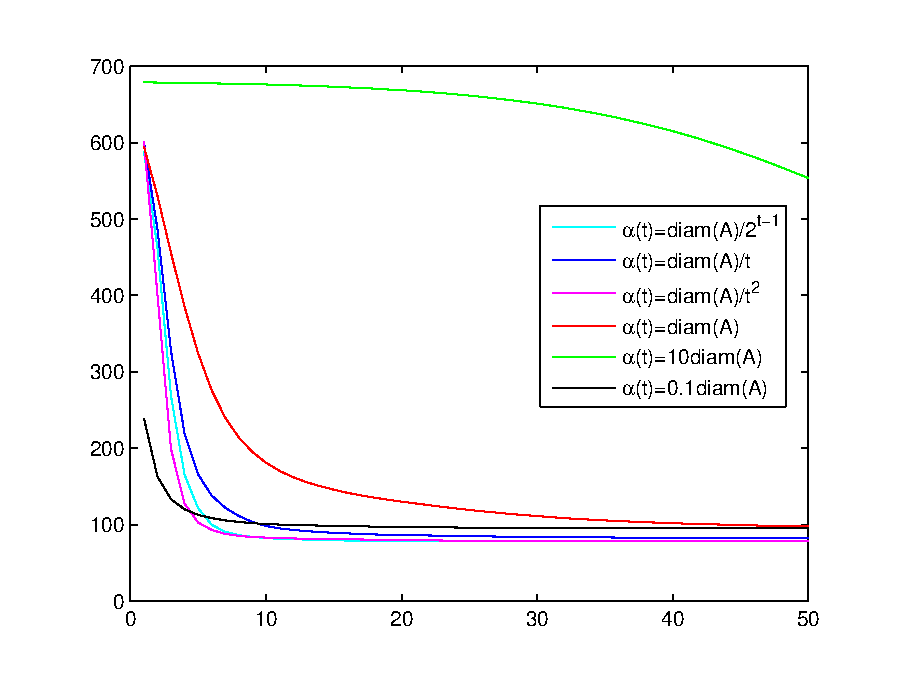
\includegraphics[width=0.8\textwidth]{dynamic_alpha_kpalm}
    \caption{Comparison of the objective values for different values of $\alpha$.}
    \label{fig:dynamic_alpha_psi_comp}
\end{figure} 

\Cref{fig:dynamic_alpha_psi_comp} shows that dynamic values of the parameter $\alpha$ which decreases fast, such as $\alpha_i(t)=
\frac{diam(\mathcal{A})}{2^{t-1}}$, achieve smaller function values.
In \Cref{fig:algs_psi_comp} we made a comparison between KPALM with dynamic rule for choosing the parameter $\alpha$, that is $\alpha_i(t)=\frac{diam(\mathcal{A})}{2^{t-1}}$, with k-means and k-means++. It demonstrates that KPALM can reach lower objective function values then k-means, and these are similar to the values achieved with KMEAN++. In addition, the KPALM++ are the objective function values achieved with KPALM when the $x$ variable is initialized as in k-means++. Unlike k-means, the objective function values KPALM converge to are more stable and less sensitive to its starting point.

%\begin{figure}[t]
%    \centering
%    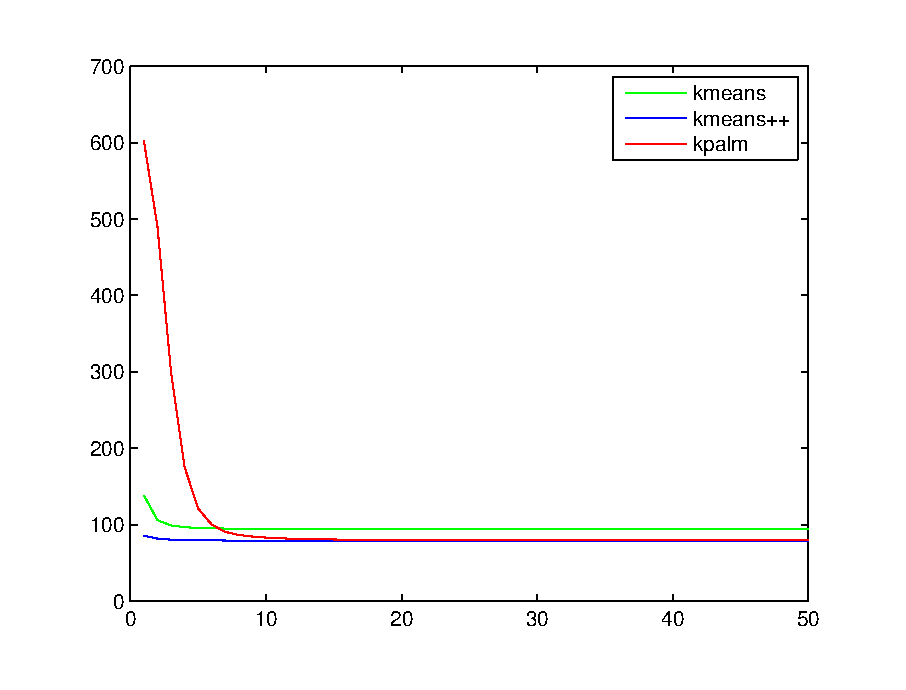
\includegraphics{psi_algs_comparison}
%    \caption{Comparison of objective function values for KMEANS, KMEANS++ and KPALM.}
%     \label{fig:algs_psi_comp}
%\end{figure}

\begin{figure}[ht]
    \centering
    \begin{subfigure}[b]{0.8\textwidth}
        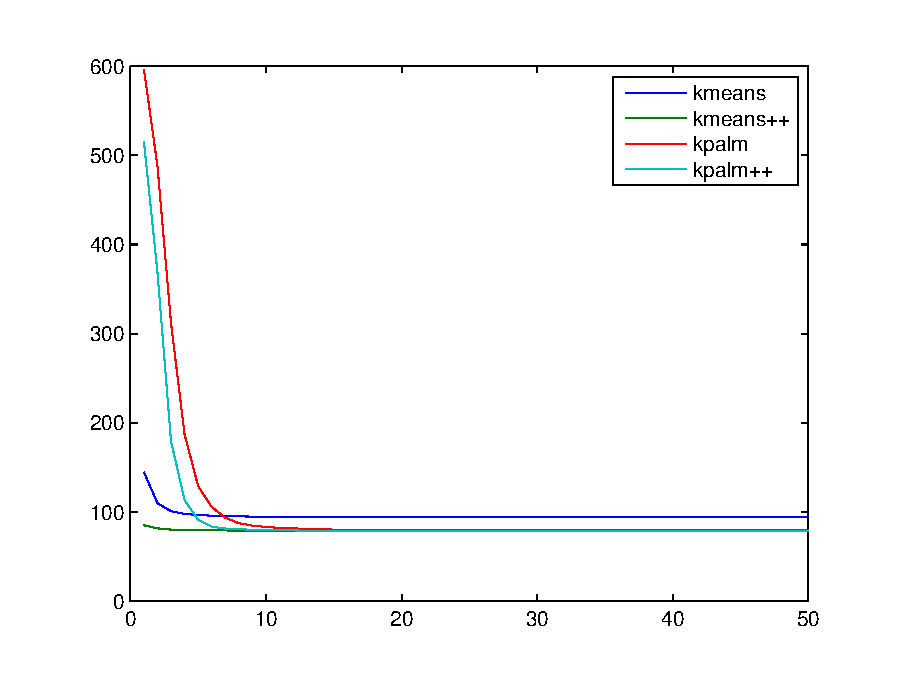
\includegraphics[width=\textwidth]{psi_algs_comparison2}
        \caption{Comparison of objective function values.}
        \label{fig:algs_psi_comp_A}
    \end{subfigure}
    \begin{subfigure}[b]{0.8\textwidth}
        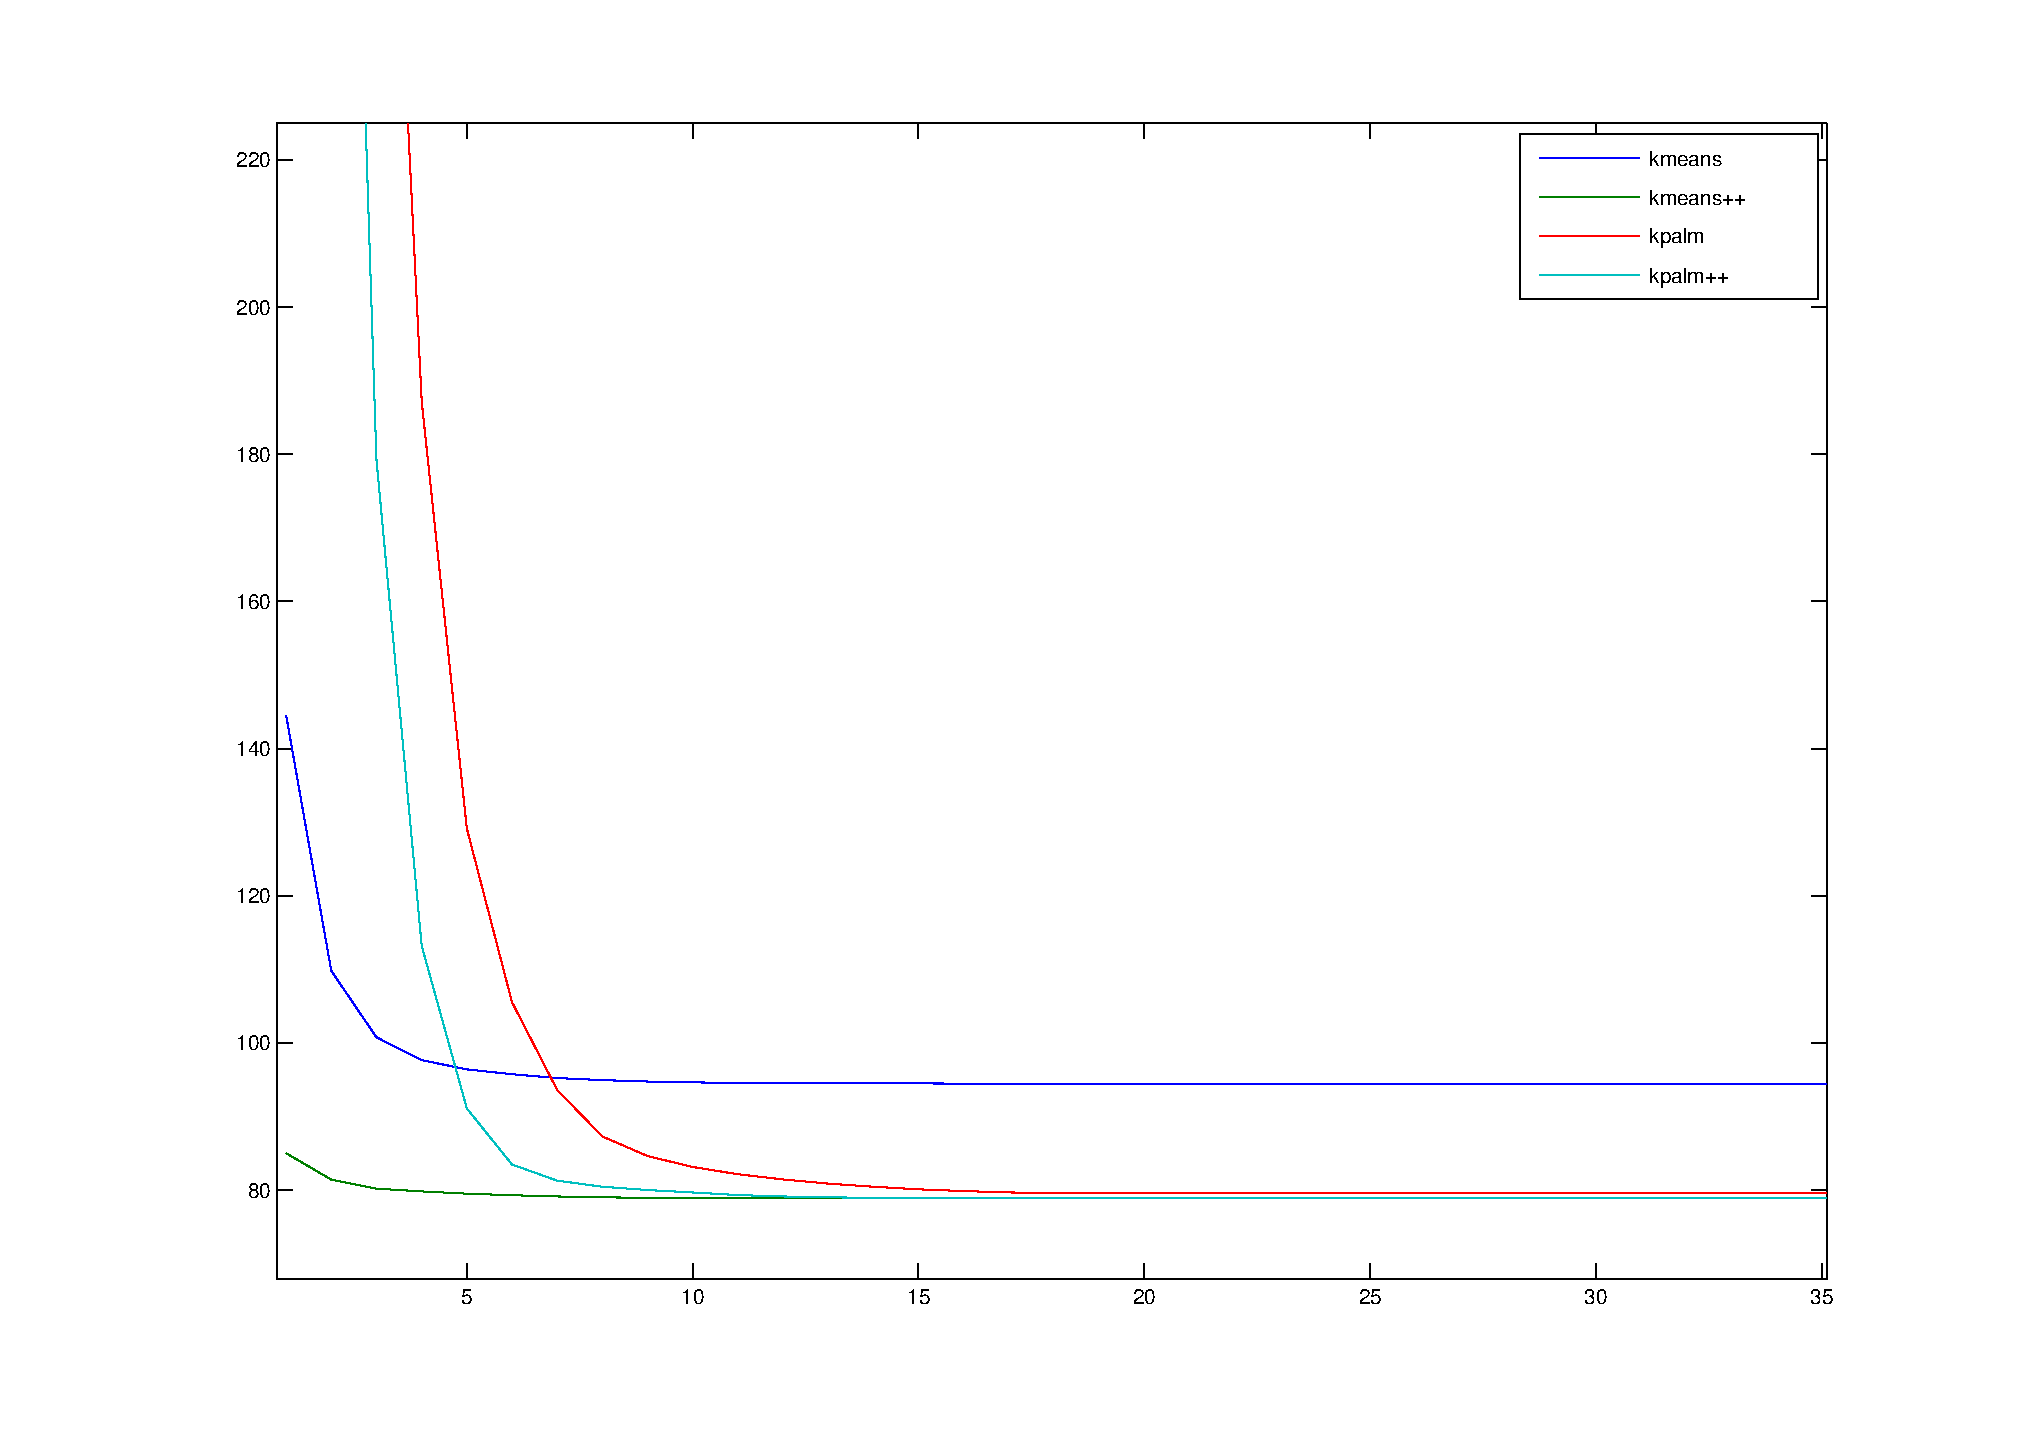
\includegraphics[width=\textwidth]{psi_algs_comparison2_zoom}
        \caption{Zoom of \Cref{fig:algs_psi_comp_A}.}
        \label{fig:algs_psi_comp_B}
    \end{subfigure}
    \caption{Comparison of objective function values for k-means, k-means++, KPALM and KPALM++.} \label{fig:algs_psi_comp}
\end{figure}

%\begin{figure}[t]
%    \centering
%    \scalebox{.5}{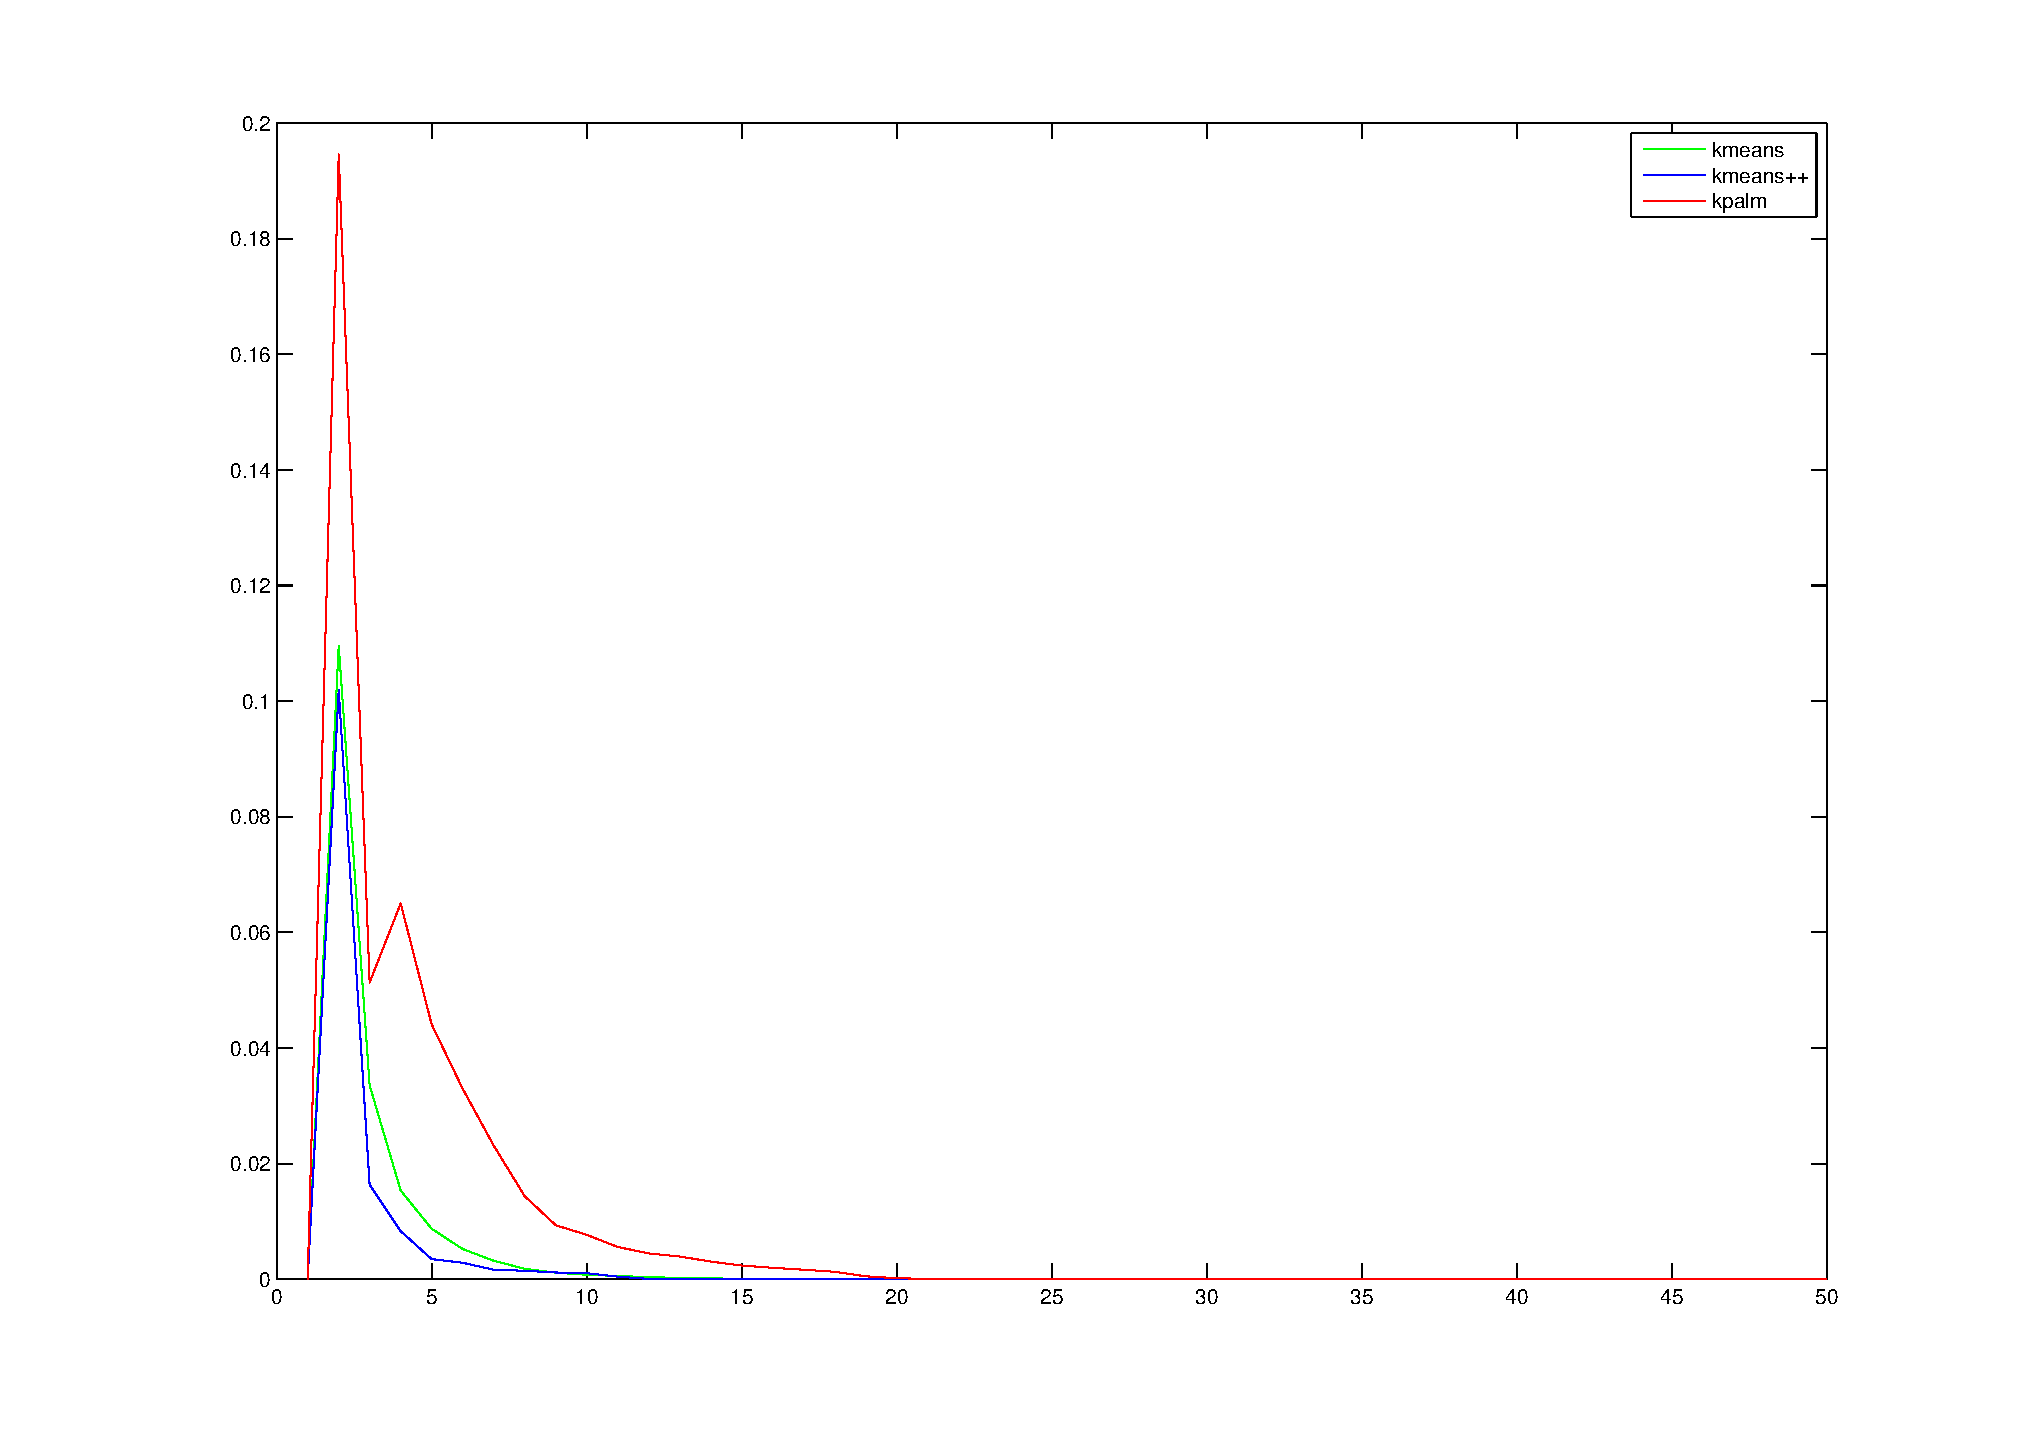
\includegraphics{relative_delta_algs_comparison}}
%    \caption{Comparison of $\frac{\|x(t+1)-x(t)\|}{\|x(t)\|}$ for KMEANS, KMEANS++ and KPALM.}
%    \label{fig:dynamic_alpha_relative_delta_comp}
%\end{figure}

\Cref{fig:iters_comp} shows the number of iteration needed to reach precision of 1e-3 between consecutive objective function values.
Similarly to \Cref{fig:dynamic_alpha_psi_comp}, in \Cref{fig:dynamic_alpha_eps_psi_comp} we can see a comparison of the objective values of $\Psi_{\varepsilon}$ for different function values. The value of $\varepsilon$ is set to be 1e-5.

\begin{figure}
    \centering
    \begin{subfigure}[b]{0.7\textwidth}
        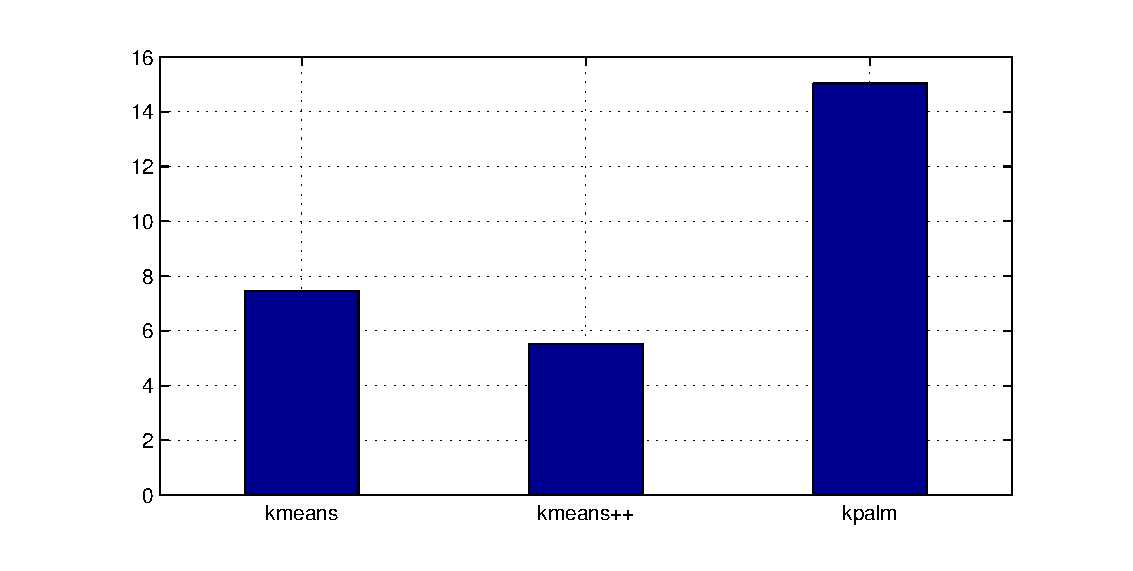
\includegraphics[width=\textwidth]{iterations_algs_comparison}
        \caption{Number of iterations of k-means, k-means++ and KPALM with $\alpha(t)=diam(\mathcal{A})/2^{t-1}$.}
        \label{fig:iters_algs_comp}
    \end{subfigure}
    ~ %add desired spacing between images, e. g. ~, \quad, \qquad, \hfill etc. 
      %(or a blank line to force the subfigure onto a new line)
    \begin{subfigure}[b]{0.7\textwidth}
        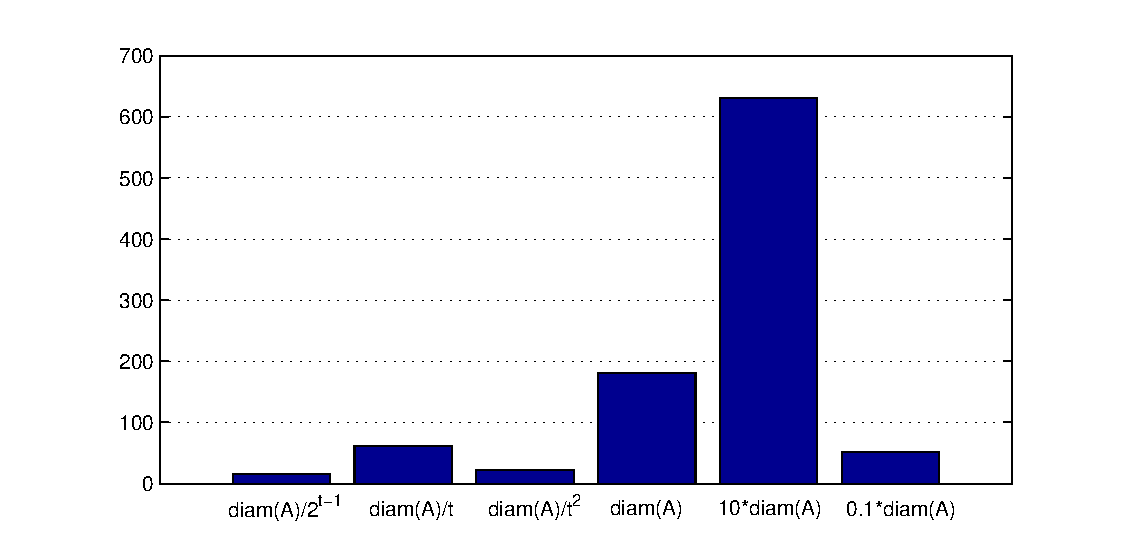
\includegraphics[width=\textwidth]{iterations_dynamic_alpha_kpalm_comparison}
        \caption{Number of iterations of KPALM with different updates of $\alpha(t)$.}
        \label{fig:iters_dyn_alpha_kpalm_comp}
    \end{subfigure}
    \begin{subfigure}[b]{0.7\textwidth}
        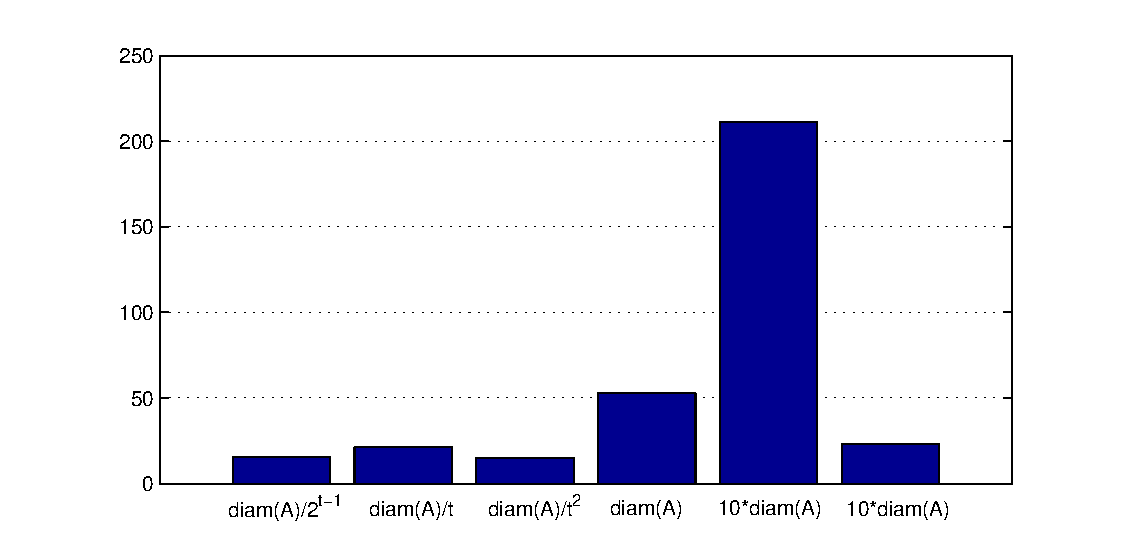
\includegraphics[width=\textwidth]{iterations_dynamic_alpha_eps_kpalm_comparison}
        \caption{Number of iterations of $\varepsilon$-KPALM with different updates of $\alpha(t)$.}
        \label{fig:iters_dyn_alpha_eps_kpalm_comp}
    \end{subfigure}
    \caption{Comparison of number of iterations needed to reach 1e-3 precision of $\Psi$.}\label{fig:iters_comp}
\end{figure}

\begin{figure}
    \centering
    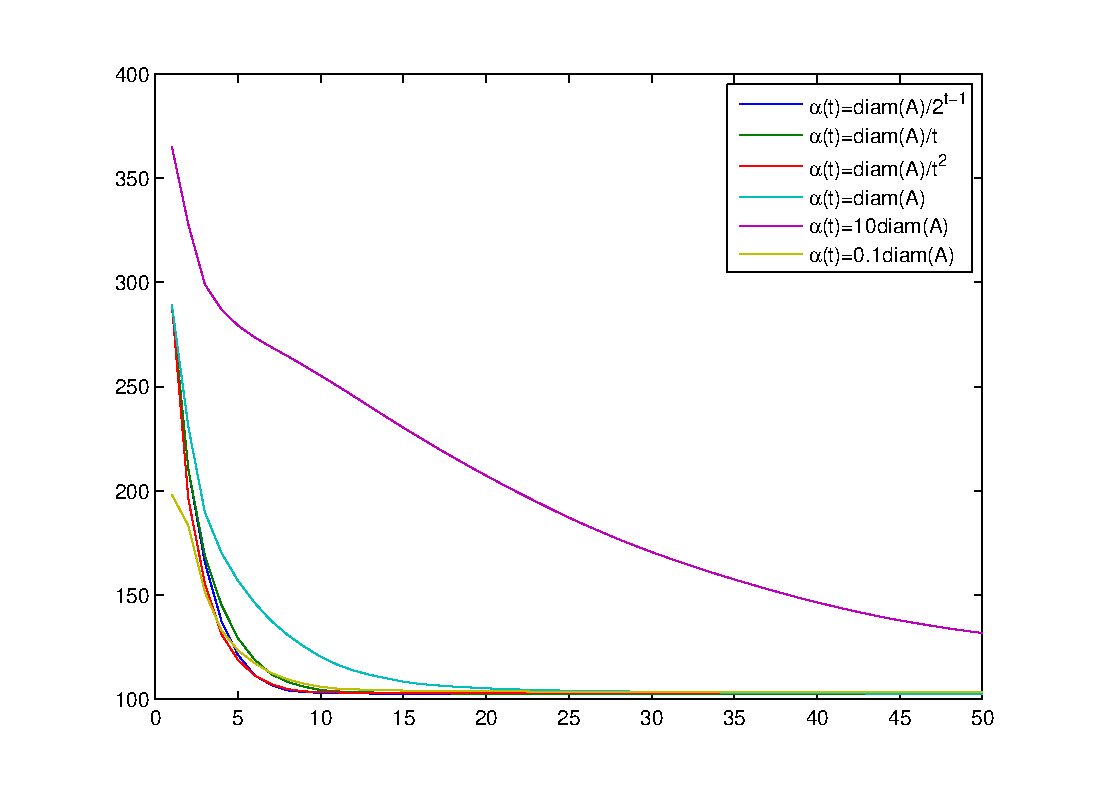
\includegraphics[width=0.75\textwidth]{dynamic_alpha_eps_kpalm}
    \caption{Comparison of the objective values for different values of $\alpha$.}
    \label{fig:dynamic_alpha_eps_psi_comp}
\end{figure}



\begin{figure}
    \centering
    \begin{subfigure}[b]{0.45\textwidth}
        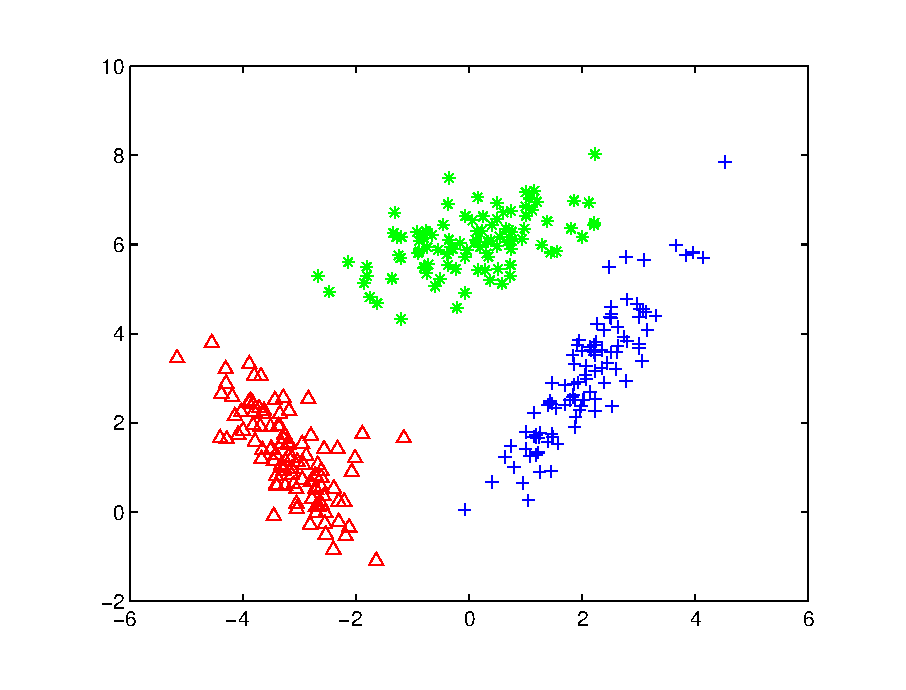
\includegraphics[width=\textwidth]{dense_gaussians}
        \caption{Dense Gaussians.}
        \label{fig:dense_gaussians}
    \end{subfigure}
    \quad
    \begin{subfigure}[b]{0.45\textwidth}
        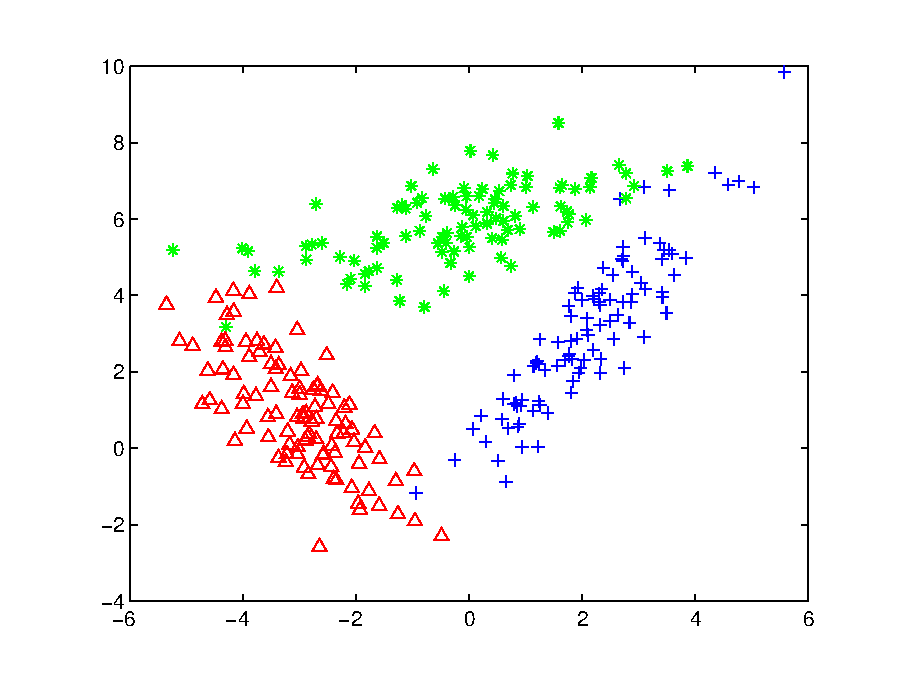
\includegraphics[width=\textwidth]{sparse_gaussians}
        \caption{Sparse Gaussians.}
        \label{fig:sparse_gaussians}
    \end{subfigure}
    \caption{Two datasets, each 300 points.}
    \label{fig:gaussians}
\end{figure}

\begin{figure}
    \centering
    \begin{subfigure}[b]{0.45\textwidth}
        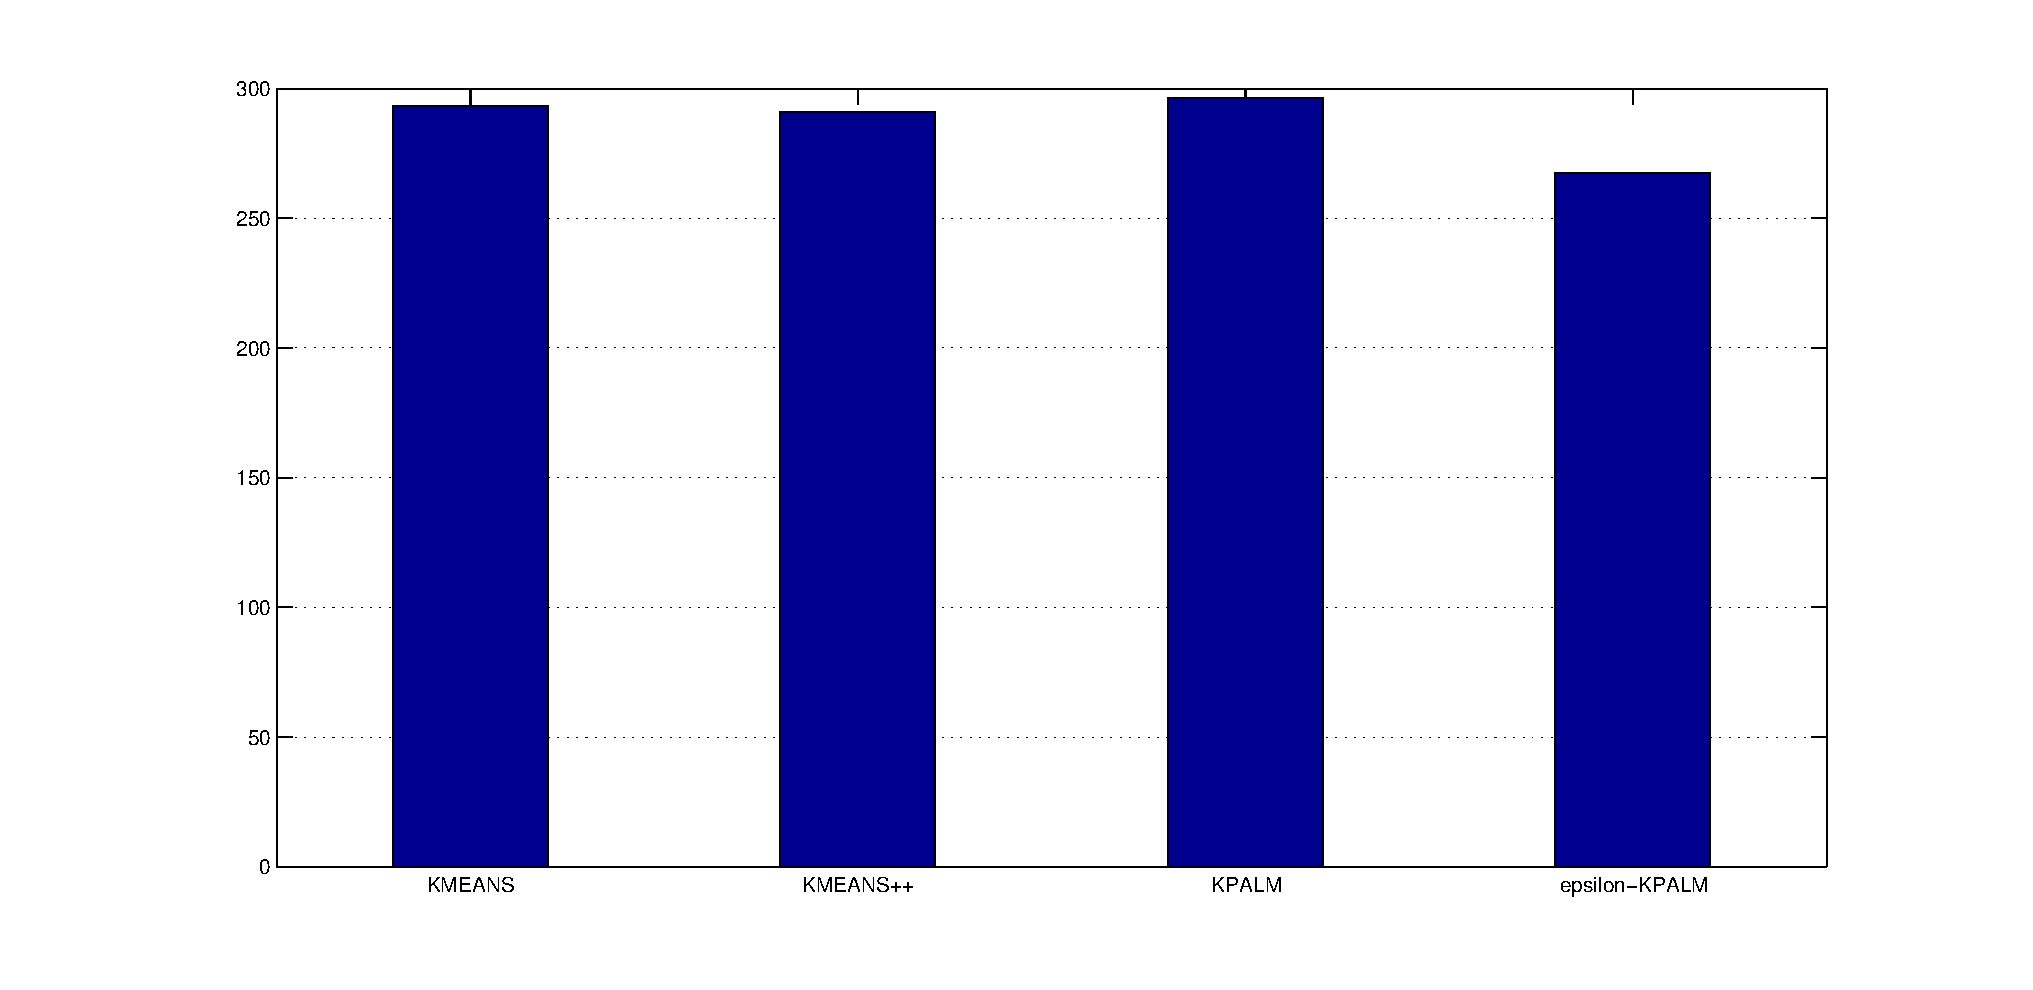
\includegraphics[width=\textwidth]{dense_gaussians_similarity}
        \caption{Dense Gaussians clustering.}
        \label{fig:dense_gaussians_similarity}
    \end{subfigure}
    \quad
    \begin{subfigure}[b]{0.45\textwidth}
        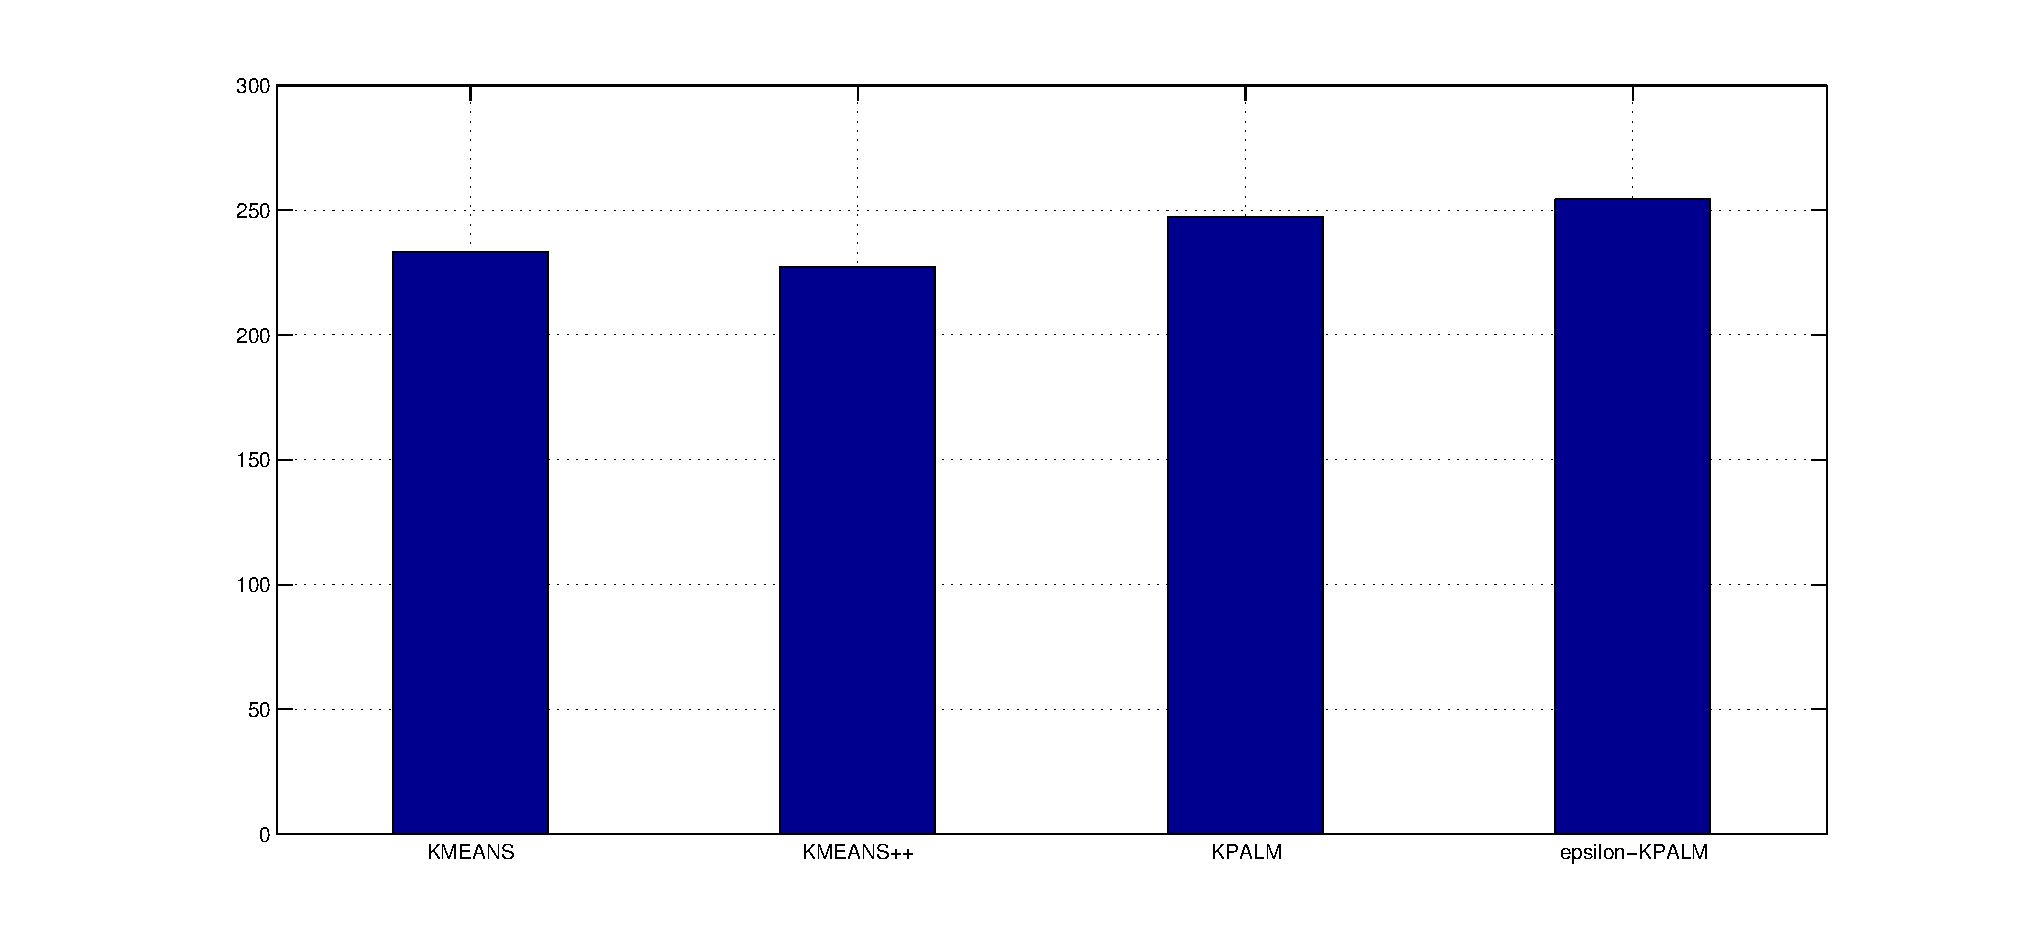
\includegraphics[width=\textwidth]{sparse_gaussians_similarity}
        \caption{Sparse Gaussians clustering.}
        \label{fig:sparse_gaussians_similarity}
    \end{subfigure}
    \caption{Results of clustering algorithms for dense and sparse datasets.}
    \label{fig:gaussians_similarity}
\end{figure}

\begin{figure}
    \centering
    \begin{subfigure}[b]{1\textwidth}
        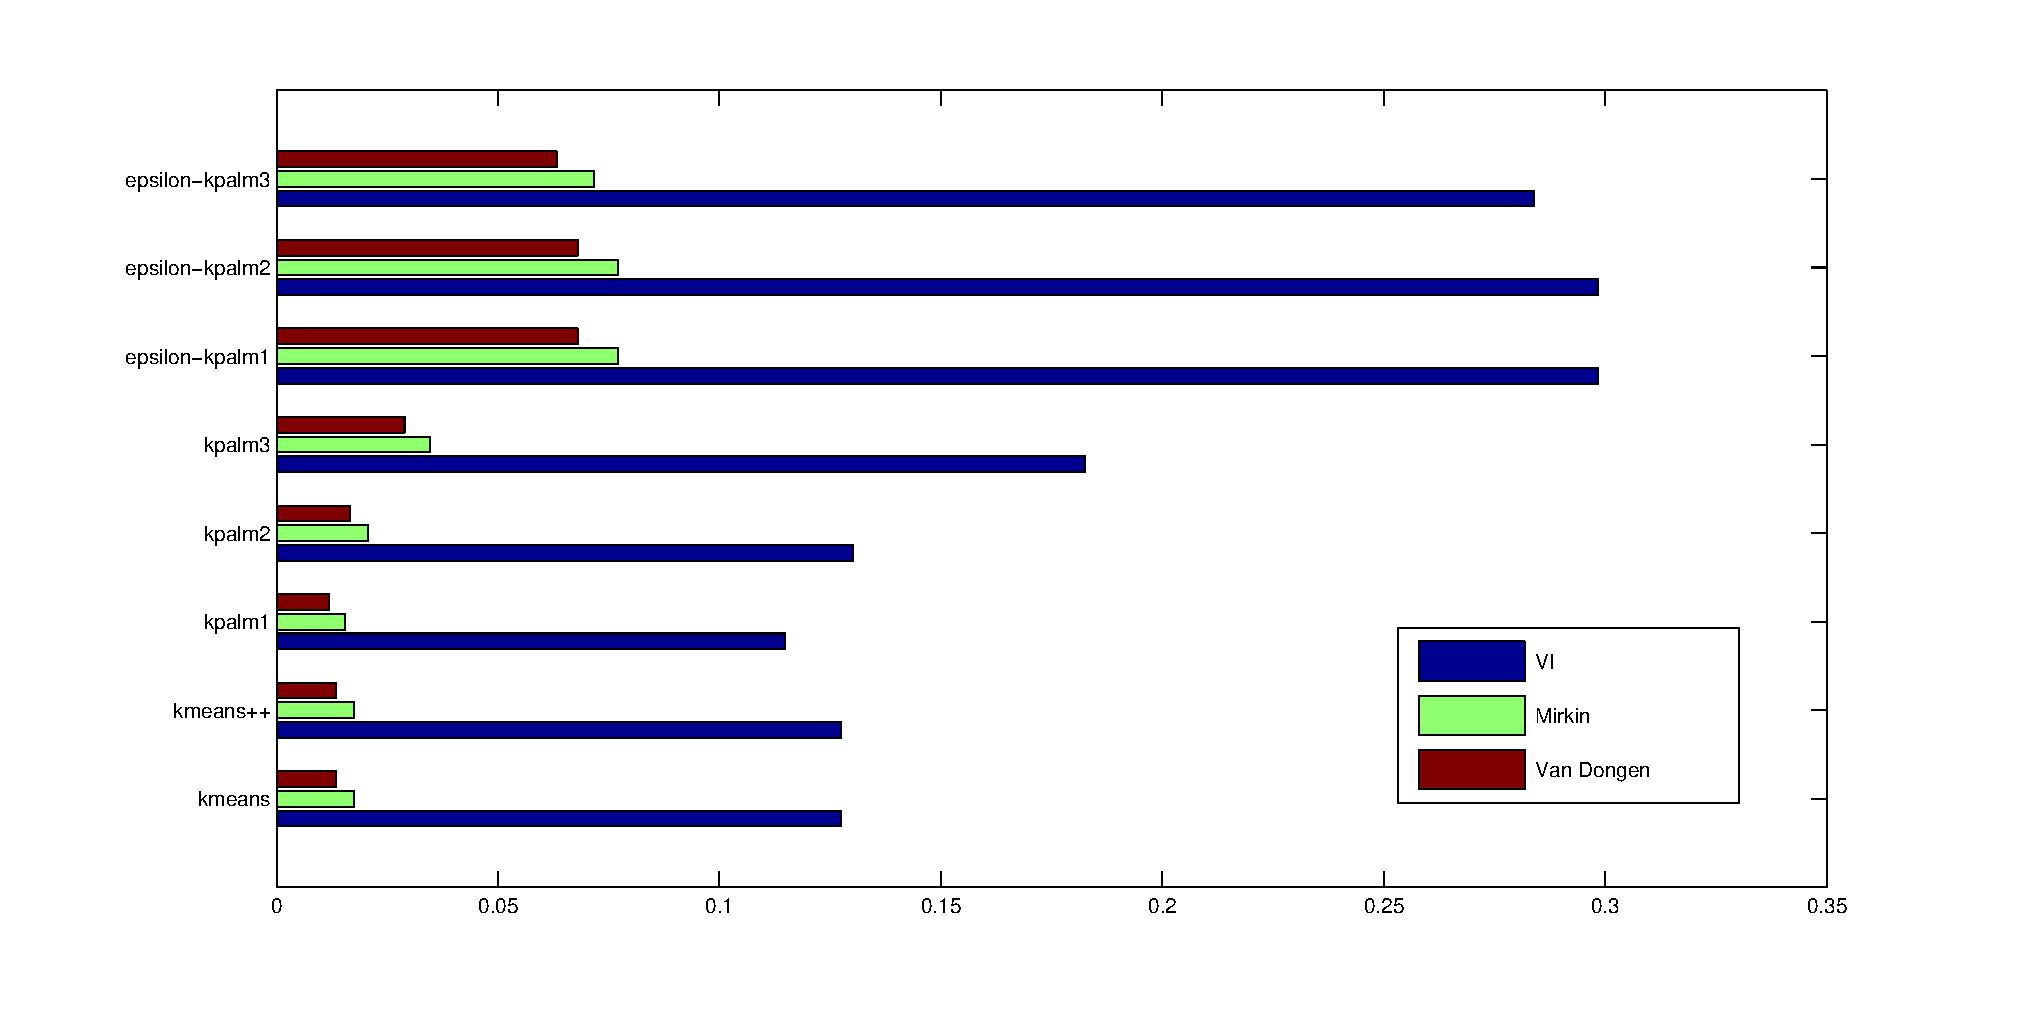
\includegraphics[width=\textwidth]{dense_gaussians_metrics2}
        \caption{Dense Gaussians metrics comparison.}
        \label{fig:dense_gaussians_metrics}
    \end{subfigure}
    \quad
    \begin{subfigure}[b]{1\textwidth}
        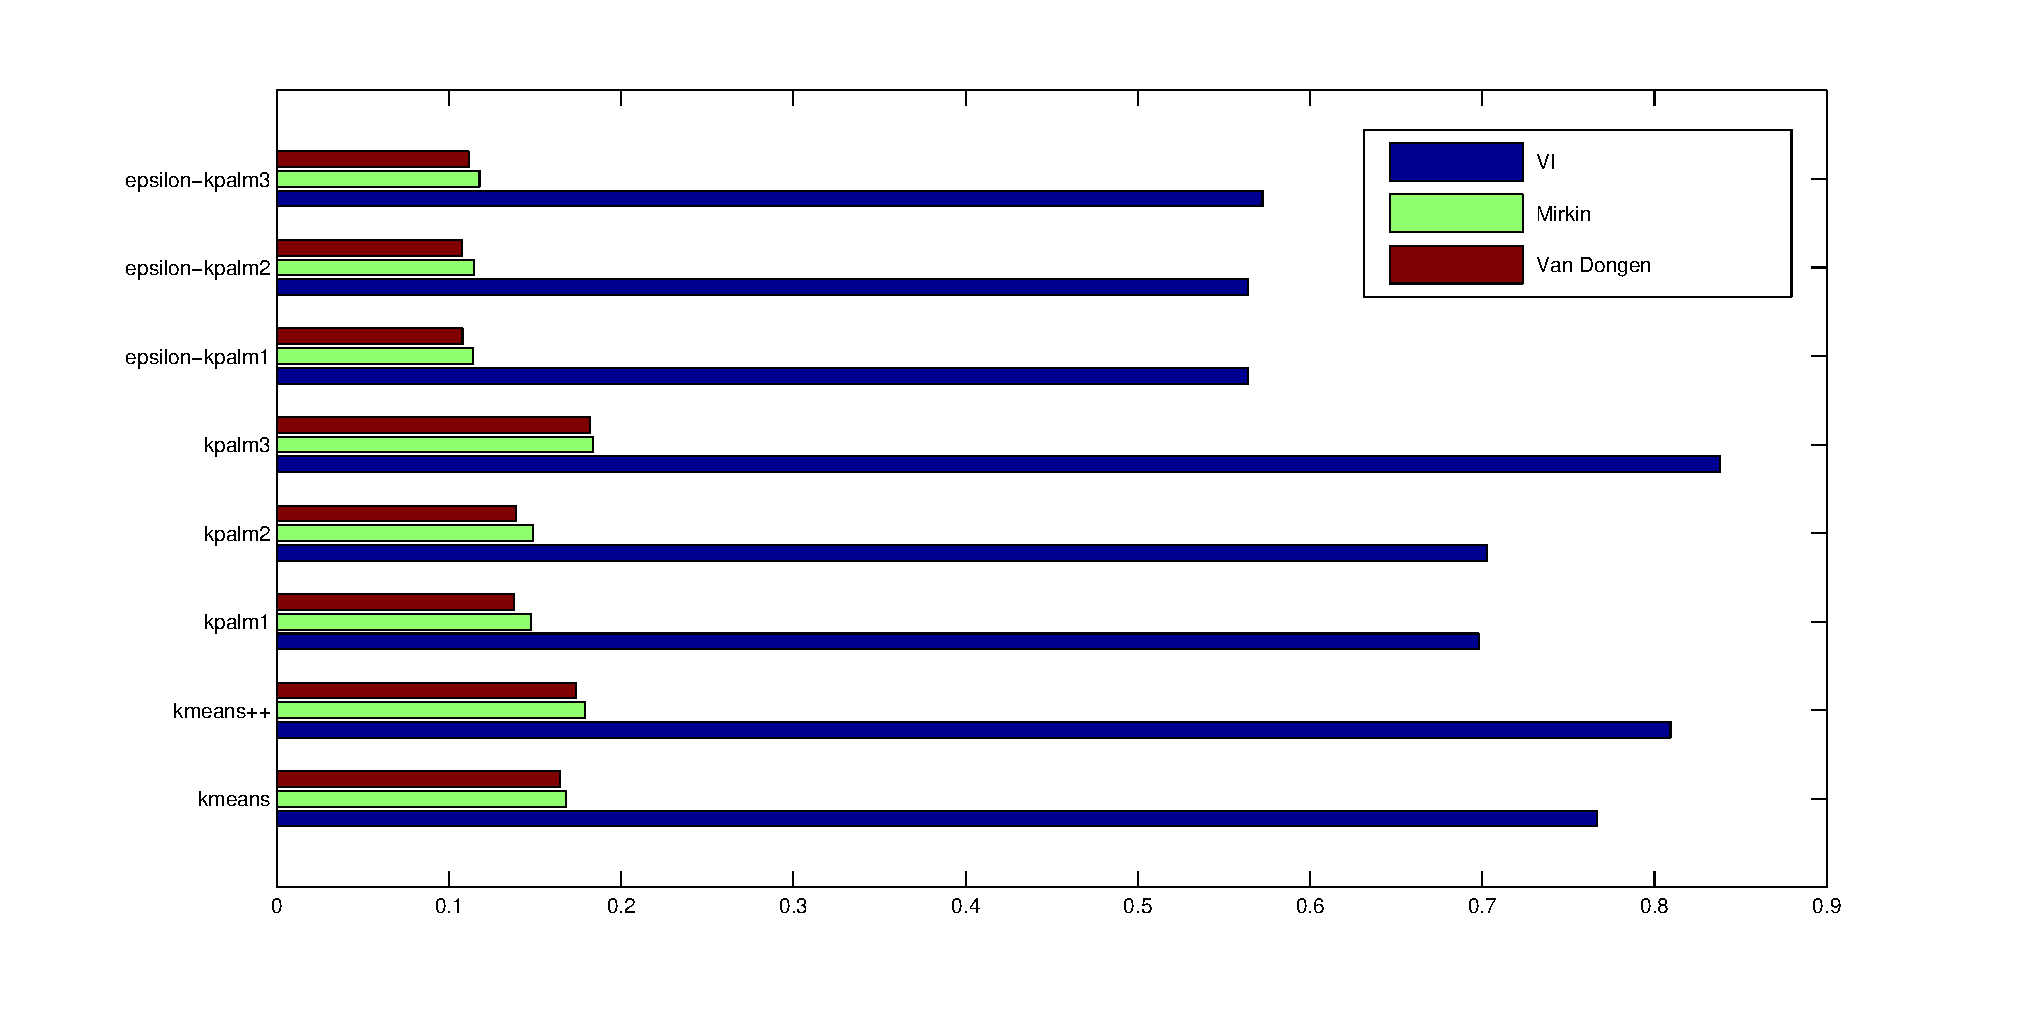
\includegraphics[width=\textwidth]{sparse_gaussians_metrics2}
        \caption{Sparse Gaussians metrics comparison.}
        \label{fig:sparse_gaussians_metrics}
    \end{subfigure}
    \caption{Comparison of metrics between clusterings for dense and sparse datasets.}
    \label{fig:gaussians_metrics}
\end{figure}

\section{Synthetic Dataset}

In this section we show that $\varepsilon$-KPALM is less sensitive to outliners in the data verses algorithms that suit the squared Euclidean norm (e.g., k-means, k-means++ and KPALM). We generated two synthetic datasets, each contains 300 points in the plane, by sampling three two-dimensional Gaussian, 100 samples each. In \Cref{fig:gaussians}(\ref{fig:dense_gaussians}) the clusters are denser than in \Cref{fig:gaussians}(\ref{fig:sparse_gaussians}).
Then we run the clustering algorithms and compared their clustering results, namely, how many points were clustered correctly. From \Cref{fig:gaussians_similarity}(\ref{fig:dense_gaussians_similarity}) it is evident that k-means is superior to other algorithms in the dense case and $\varepsilon$-KPALM is quite sensitive. Whereas, in the sparse case in \Cref{fig:gaussians_similarity}(\ref{fig:sparse_gaussians_similarity}), $\varepsilon$-KPALM is superior, and less sensitive to outliners. In \Cref{fig:gaussians_metrics} we compare the distance of clusterings achieved with different algorithms to the desired clustering, where kpalm1, kpalm2 and kpalm3 match using $\alpha(t)=diam(\mathcal{A})/2^{t-1}$, $\alpha(t)=diam(\mathcal{A})/t^2$ and $\alpha(t)=diam(\mathcal{A})$ respectively, and similarly for $\varepsilon$-kpalm$i$, $i \in \{1,2,3\}$. In \Cref{fig:gaussians_metrics}(\ref{fig:dense_gaussians_metrics}) we witness that for dense dataset, the resulting clusterings of squared Euclidean algorithms, namely, k-means, k-means++ and KPALM, are superior to the clustering $\varepsilon$-KPALM, where KPALM with $\alpha(t)=diam(\mathcal{A})/2^{t-1}$ gives the best result, that is, the clustering in this setting is the closest to the desired clustering. Whereas in the sparse dataset, the clustering achieved with $\varepsilon$-KPALM with $\alpha(t)=diam(\mathcal{A})/t^2$ is the closest to the desired clustering, as reflected from \Cref{fig:gaussians_metrics}(\ref{fig:sparse_gaussians_metrics}).


\newpage

%------------REFERRENCES------------------------------------------

\begin{thebibliography}{99}



%\bibitem{bert-82} D. P. Bertsekas. \emph{Constrained Optimization and Lagrange Multiplier Methods}.
%Academic Press, New York (1982).
%
%
%
%\bibitem{tebo-JMLR07} M. Teboulle. A unified continuous optimization framework
%for center-based clustering methods. \emph{Journal of Machine Learning Research}, Vol. 8, pp. 65-102 (2007).


\bibitem{AB2009} H. Attouch, J. Bolte. On the convergence of the proximal algorithm for nonsmooth functions involving analytic features. \emph{Math. Program.}, Vol. 116, pp. 5-16 (2009).


\bibitem{ABS2013}  H. Attouch, J. Bolte, B.F. Svaiter. Convergence of descent methods for semi-algebraic and tame problems: proximal algorithms, forward-backward splitting, and regularized Gauss-Seidel methods. \emph{Math. Program.}, Vol. 137, 91-129 (2013).


\bibitem{BS2015} A. Beck, S. Sabach. Weiszfeld's Method: Old and New Results. \emph{Journal of Optimization Theory and Applications}, Vol. 164, pp. 1-40 (2015).


\bibitem{ATY1991} A. Ben-Tal, M. Teboulle, W.H. Yang. A least-squares-based method for a class of nonsmooth minimization problems with applications in plasticity.  \emph{Applied Mathematics and Optimization}, Vol. 24, pp. 273-288 (1991).


\bibitem{BST2014} J. Bolte, S. Sabach, M. Teboulle. Proximal alternating linearized minimization for nonconvex and nonsmooth problems. \emph{Math. Program.}, Vol. 146, pp. 459-494 (2014).


\bibitem{M2005} M. Meila. Comparing Clusterings - An Axiomatic View. \emph{In ICML '05: Proceedings of the 22nd international conference on Machine Learning ACM}, New York, pp. 577-584 (2005).


\bibitem{SI1984} S.Z. Selim,  M.A. Ismail. K-Means-Type Algorithms. A Generalized Convergence Theorem and Characterization of Local Optimality. \emph{IEEE Transactions on Pattern Analysis and Machine Intelligence}, Vol. 6, pp. 81-87 (1984).


\bibitem{T2007} M. Teboulle. A Unified Continuous Optimization Framework for Center-Based Clustering Methods. \emph{The Journal of Machine Learning Research}, Vol. 8, pp. 65-102 (2007).

\end{thebibliography}

\end{document}
